%%
%% This is file `thesis.tex',
%% generated with the docstrip utility.
%%
%% The original source files were:
%%
%% nudtpaper.dtx  (with options: `thesis')
%% 
%% This is a generated file.
%% 
%% Copyright (C) 2015 by Liu Benyuan <liubenyuan@gmail.com>
%% 
%% This file may be distributed and/or modified under the
%% conditions of the LaTeX Project Public License, either version 1.3a
%% of this license or (at your option) any later version.
%% The latest version of this license is in:
%% 
%% http://www.latex-project.org/lppl.txt
%% 
%% and version 1.3a or later is part of all distributions of LaTeX
%% version 2004/10/01 or later.
%% 
%% To produce the documentation run the original source files ending with `.dtx'
%% through LaTeX.
%% 
%% Any Suggestions : LiuBenYuan <liubenyuan@gmail.com>
%% Thanks Xue Ruini <xueruini@gmail.com> for the thuthesis class!
%% Thanks sofoot for the original NUDT paper class!
%% 
%1. 规范硕士导言
% \documentclass[master,ttf]{nudtpaper}
%2. 规范博士导言
% \documentclass[doctor,twoside,ttf]{nudtpaper}
%3. 建议使用OTF字体获得较好的页面显示效果
%   OTF字体从网上获得,各个系统名称统一。
%   如果你下载的是最新的(1201)OTF英文字体,建议修改nudtpaper.cls,使用
%   Times New Roman PS Std
% \documentclass[doctor,twoside,otf]{nudtpaper}
%   另外,新版的论文模板提供了方正字体选项FZ,效果也不错哦
% \documentclass[doctor,twoside,fz]{nudtpaper}
%4. 如果想生成盲评,传递anon即可,仍需修改个人成果部分
% \documentclass[master,otf,anon]{nudtpaper}
%
\documentclass[doctor,twoside,otf]{nudtpaper}
\usepackage{mynudt}
\usepackage{tabu}
\usepackage{makecell}
\usepackage{placeins}
\usepackage[]{xcolor}
%\usepackage{ctex}



\classification{TP391.4}
\serialno{13069014}
\confidentiality{公开}
\UDC{004.93}
\title{基于异构平台的典型应用的并行优化技术研究}
\displaytitle{基于异构平台的典型应用的并行优化技术研究}
\author{蓝强}
\zhdate{二〇一七\ 年\ 十\ 月}
\entitle{Research on Parallell Optimization Techniques for Typical Applications Based on Heterogeneous Platform}
\enauthor{Lan Qiang}
\endate{May 26, 2017}
\subject{计算机科学与技术}
\ensubject{Computer Science and Technology}
\researchfield{高性能计算}
\supervisor{王意洁\quad{}教授}
%\cosupervisor{王五\quad{}副教授} % 没有就空着
\ensupervisor{Prof. Wang Yijie}
%\encosupervisor{}
\papertype{工学}
\enpapertype{Engineering}
% 加入makenomenclature命令可用nomencl制作符号列表。
%\makenomenclature

\begin{document}
\graphicspath{{figures/}}
% 制作封面,生成目录,插入摘要,插入符号列表 \\
% 默认符号列表使用denotation.tex,如果要使用nomencl \\
% 需要注释掉denotation,并取消下面两个命令的注释。 \\
% cleardoublepage% \\
% printnomenclature% \\
\maketitle
\frontmatter
\tableofcontents
\listoftables
\listoffigures

\cleardoublepage
%\printnomenclature

\midmatter
\begin{cabstract}
各种应用需求促使了大量的异构平台的涌现。典型的异构平台加速器包括数字信号处理器(DSP)、面向通用计算的图像处理器(GPU)、众核协处理器(MIC)以及硬件加速器(FPGA)等。

针对异构平台的编程优化面临诸多挑战。由于各种异构平台体系结构的差异,所采用的编程方法以及并行优化方法都将不同。针对GPU这种含有大量并行计算单元并以SIMT方式执行的异构平台,编程实现中,需要特别注意避免条件分支语句的使用和优化。而对众核协处理器(MIC)这种异构平台,由于cache大小受限,因此在对应用实现中需要注意访存优化。异构平台中CPU和加速器间的协同和通信问题也是对异构平台性能发挥至关重要的因素。%,因此,也是编程优化需要解决的问题。其它异构平台也面临相似的问题。

异构平台在科学计算和人工智能领域逐渐发挥越来越重要的作用。本课题分别从科学计算(心脏组织模拟)和人工智能领域(卷积神经网络)各选取一个典型应用在异构平台上进行映射。无论是心脏组织模拟应用还是卷积神经网络应用,对计算需求都非常大,其中包含的计算也有各自的特点,根据计算特点,本课题选取了两种典型的异构平台进行实现,一种是基于Intel Xeon Phi加速器的异构平台,一种是基于Nvidia GPU的异构平台。主要涉及的研究内容包括以下几方面:
\begin{compactitem}
\item[1.]心脏组织的3D模拟在大规模多核CPU系统上的映射。目前关于心脏模拟的研究都集中在2D规模,或者针对单个心脏细胞内的研究,本课题提出了一个精细的3D心脏组织模拟模型,这个模型能够模拟人类心脏组织细胞内的电活动和钙离子处理过程。%本课题最终是要将心脏组织的3D模拟映射到大规模异构系统中,具体的系统为天河2号系统,对于大规模异构集群系统来说,各节点的主机CPU的性能也不能忽略,因此
本课题首先针对大规模集群的多核CPU系统进行并行优化。采用MPI并行编程方法将心脏组织划分成很多小网格并分配到每个计算节点中,在每个计算节点内部,面向多核CPU采用OpenMP并行编程技术将分配给每个计算节点的心脏组织细胞进行任务划分,最后单核CPU在对单个心脏细胞内的模拟中,采用SIMD技术进一步对细胞内的dyad单元实现并行计算。本课题采用多种并行技术高效地将心脏组织的3D模拟映射到了大规模多核CPU的集群系统中。

\item[2.]心脏组织的3D模拟在天河2号超级计算系统上的映射。在大规模多核CPU系统上实现了心脏组织的3D模拟后,本课题将心脏组织的3D模拟扩展到天河2号超级计算系统上,天河2号系统中的每个计算节点是由多核CPU与3个Intel Xeon Phi加速器构成的,在天河2号系统的异构节点间的任务划分方法与在大规模多核CPU系统上划分方法类似,都是采用MPI方法进行任务划分,但在天河节点内的任务划分,本课题根据天河节点内多核CPU与Intel Xeon Phi在计算心脏细胞的实际性能进行任务划分,确保多核CPU与Xeon Phi间的负载均衡,在Xeon Phi加速器上的映射中,同样采用了OpenMP并行以及SIMD向量化技术。而对于CPU和Xeon Phi间的协同,本课题采用的是COI/SCIF底层编程接口,在CPU端通过调用COI接口实现对Xeon Phi的控制,而通过SCIF接口实现CPU与Xeon Phi间的数据通信。

\item[3.]3D卷积神经网络在异构GPU平台上的高性能实现。2D卷积神经网络已经在很多应用中取得了很好的效果,但3D卷积神经网络目前并没有应用的很广泛,主要受限于3D卷积神经网络计算量大的因素。因此本课题针对目前3D卷积网络中卷积计算量大的问题,推导出了一种能够有效降低计算量的3D卷积算法,即3D Winograd算法。该算法的原理是通过对卷积层的输入和卷积核进行变换,将变换后的结果进行矩阵乘运算,然后将运算结果再反变换回最后的结果,通过引入几个变换来减少矩阵乘的规模。本课题从理论上证明了该算法能有效降低浮点运算量,并在GPU异构平台上高效地并行实现,主要是通过CUDA编程将该算法中涉及的几个变换过程映射到GPU中,映射过程中采用了对齐访问和减少访存次数两种优化技术提高变换过程在GPU的性能,而对3D Winograd算法中的矩阵乘部分则通过调用目前比较成熟的cublas库实现,最后取得了比当前流行的深度学习库更好的性能。

\item[4.]面向卷积神经网络前向过程的低延迟实现。低延迟在很多应用场景中作为卷积神经网络前向过程的一个重要指标,为了降低计算时间,本课题在多GPU设备上对卷积神经网络采用模型并行进行加速。模型并行中,每一层卷积层的计算都被分割到多个设备中执行,每个设备负责计算卷积层的部分输出结果,各个设备计算出的部分输出结果需要合并作为下一层的输入,因此,模型并行需要解决设备间的通信问题,本课题设计了一个高效的通信模式,一方面降低通信时间,另一方面尽量隐藏通信时间。

\end{compactitem}

综上所述,本课题选取的两个典型应用都为计算密集型的应用,适合在异构平台下进行加速,而本课题根据心脏组织模拟与卷积神经网络计算中各自不同的特点分别将它们映射到不同类型的异构平台中。在具体的映射过程中,提出了一些算法的改进并对各种并行技术进行了研究与实现。

\end{cabstract}
\ckeywords{ 异构平台;数字信号处理器;众核协处理器;科学计算;心脏组织模拟;卷积神经网络;3D Winograd;低延迟}

\begin{eabstract}
The demand of applications makes heterogenous platform widespread. The accelerator-based heterogenous system means a computer system connected with different functional or performance computing device, one of the computing device called accelerator outperforms traditional general processor, the accelerator is used for accelerating the compute-intensive part of an application. Typical accelerator include digital signal processor(DSP), graph processor for general computing, many-core coprocessor(MIC) and hardware accelerator(FPGA) etc.

Programming optimization for heterogenous platform meets lots of challenges. The difference of architecture between each heterogenous platform causes difference in programming methods and parallel optimization methods. For heterogenous platform like GPU which has lots of parallel compute units and execute in SIMT way, application developer should pay special attention to avoid using conditional branch statements in the implementations. However, for platform like many-core coprocessor(MIC), which is limited by its cache size, it is important to optimize memory accessing while programming. The coordination and communication between CPU and accelerator are also key to make full use of the heterogenous platform, which is also one problem to solve while programing optimization. Those problems also occur in other heterogenous platforms. 

Heterogenous platform are becoming more and more important in scientific computing and artificial intelligence field. The research program choose cardiac tissue simulation and convolutional neural network as typical application representation in science computing and artificial intelligence field respectively, these two applications are implemented on heterogenous platform. Either cardiac simulation or convolutional neural network demands lots of computing resources, and has its own features in computing, the research program choose two different heterogenous platform to implement according their computing features, one is based on Intel Xeon Phi accelerator and the other is based on Nvidia GPU platform.  Main research work include following lists:
\begin{compactitem}
\item[1.]3D simulation of cardiac tissue on large scale multi-core CPU system. Most of research on cardiac simulation focus on 2D simulation, or single cell, our research program propose a detailed 3D cardiac tissue simulation model, which simulates the electrical activity and calcium handling at the tissue level. The research program aims to implement 3D cardiac tissue simulation on large scale heterogenous platforms like Tianhe-2 system. The performance of host CPU in heterogenous platform can not be ignored. The research program work on large scale multi-core CPU system first. MPI programming method is used to divide task among all the computing nodes, while OpenMP parallel programming technique is used to divide computing task among multi-cores on each computing node. Finally, SIMD vectorization is applied to parallel the computing task happened inside cardiac cells on each CPU core. Therefor, we adopted multiple parallelization techniques to implement the 3D cardiac tissue simulation on large scale multi-core CPU system.

\item[2.]Implementation of 3D cardiac tissue simulation on Tianhe-2 super computing system. Based on the implementation of 3D cardiac tissue simulation on large scale multi-core system, we extend the work to Tianhe-2 super computer system, each node on Tianhe-2 system contains multi-core CPUs and 3 Intel Xeon Phi accelerators, the tasks dividing method among Tianhe-2 nodes is the same as among large scale CPU system, both of which adopt MPI method. However, for the task dividing method among node level, we divide task depending on the computing capacity of multi-core CPU and Xeon Phi to guarantee load balancing between CPU and Xeon Phi. And like on multi-core CPU, both OpenMP and SIMD methods are used on Xeon Phi device. For the coordination between CPU and Xeon Phi, we exploit COI/SCIF low level programming interface, we call COI interface on CPU side to control Xeon Phi device and call SCIF interface to implement the communication between CPU and Xeon Phi device.

\item[3.]High performance implementation of 3D CNN(convolutional neural network) on GPU platform. 2D convolutional neural network play good role in many applications, however, we do not observe widespread use of 3D CNN, because of huge computation needed in 3D CNN. We derive a new algorithm called 3D Winograd to compute 3D convolution operation and the new algorithm can reduce computation obviously. The principle of 3D Winograd algorithm is transforming the input and filters of a convolutional layer, applying matrix multiplication to the transformed results and then transforming the result of matrix multiplication back. The transforming operation can increase some computation, however, the matrix multiplication reduce computation more obviously. We prove that 3D Winograd algorithm can reduce computation in theory. We implement the algorithm on GPU efficiently, we use CUDA programming method to implement those transforming tasks and adopt two optimization techniques which are memory align accessing and reducing the number of memory access to improve the performance on GPU, for the matrix multiplication in the 3D Winograd algorithm, we call cublas library to implement that, finally, we achieve better performance than some popular deep learning library.

\item[4.]Low latency implementation for the inference phase of convolutional neural network. Low latency of the inference phase of convolutional neural network is one important factor in many applications, to reduce the computing time, we exploit model parallelization technique to accelerate CNN on multiple GPU devices. The computation task of Each convolutional layer is divided among multiple devices in model parallelization, each device is only responsible for computing part of the results, and these results are merged as the input of next layer, therefore, communication between devices are needed to solve during the model parallelization, we design a efficient communication mode which can reduce the communication time and also is convenient to overlap communication and computing. 

\end{compactitem}

In summary, these two typical applications chosen by the research program are both computing intensive application, according to the computing features of these two application, we implement them on different heterogenous platforms. During the implementations, we propose new algorithm and study many parallelization techniques. 
\end{eabstract}
\ekeywords{ Heterogenous Platform; Digital Signal Processor; Many-core Coprocessor; Scientific Computing; Cardiac Tissue Simulation; Convolutional Neural Network; 3D Winograd; Low Latency}

%\chapter*{符号使用说明}
% 可以根据需要在chapter后加星星/去掉星星

\begin{denotation}

\item[HPC] 高性能计算 (High Performance Computing)
\item[cluster] 集群
\item[Itanium] 安腾
\item[SMP] 对称多处理
\item[API] 应用程序编程接口
\item[PI]	聚酰亚胺
\item[MPI]	聚酰亚胺模型化合物,N-苯基邻苯酰亚胺
\item[PBI]	聚苯并咪唑
\item[MPBI]	聚苯并咪唑模型化合物,N-苯基苯并咪唑
\item[PY]	聚吡咙
\item[PMDA-BDA]	均苯四酸二酐与联苯四胺合成的聚吡咙薄膜
\item[$\Delta G$]  	活化自由能~(Activation Free Energy)
\item [$\chi$] 传输系数~(Transmission Coefficient)
\item[$E$] 能量
\item[$m$] 质量
\item[$c$] 光速
\item[$P$] 概率
\item[$T$] 时间
\item[$v$] 速度

\end{denotation}



%书写正文,可以根据需要增添章节; 正文还包括致谢,参考文献与成果
\mainmatter


%*********************第一章******************
\chapter{绪论}

\section{研究背景和意义}


\subsection{心脏组织模拟}


\subsection{卷积神经网络应用与加速}


\subsection{异构平台及异构编程}


\section{研究现状}

\subsection{心脏组织模拟数学模型的研究现状}


\subsection{卷积神经网络快速实现的相关研究}


\subsection{针对异构平台的并行优化技术研究}


\section{主要研究内容和创新点}


\section{论文结构}







%*********************第二章******************
\chapter{基于大规模多核CPU系统的心脏组织的3D精细模拟}
\label{ICA3PP}

\section{引言}
细胞内钙离子处理功能异常被认为是几个心脏病理(比如心脏衰竭\upcite{marks2013calcium,kubalova2005abnormal},心脏肥大\upcite{berridge2006remodelling},心肌病\upcite{pieske1995alterations}以及肌浆网内钙离子释放处理紊乱\upcite{liu2006arrhythmogenesis,priori2011inherited})的极有可能的诱因。上述心脏疾病中的大多都是源于亚细胞内微米级和纳米级上钙离子释放处理功能不正常造成的,表现为由t-型管畸形\upcite{louch2004reduced,louch2006t,van2011disrupted}和单兰尼碱受体功能紊乱\upcite{liu2006arrhythmogenesis,jiang2005enhanced}造成心脏的病理。

在过去的几年里,数值方法和计算技术的进步使得心脏细胞的电生理学和钙离子处理模型得到了快速发展,这些模型也开始考虑亚细胞中的随机钙离子释放过程\upcite{restrepo2008calsequestrin,gaur2011multiscale,nivala2012computational,williams2011dynamics}的离散特性。新一代的钙离子处理和动作电位模型在研究心律失常的机制和预防具有非常重要的价值,心律失常主要因为细胞内纳米级钙离子释放通道和dyadic单元功能的紊乱进而影响亚细胞级的膜电位的不正常而造成的,膜电位的异常通常表现为去极化延迟、过早地去极化\upcite{song2015calcium}以及心脏电交替变化\upcite{restrepo2008calsequestrin,nivala2012calcium,nivala2015t}。虽然这些发展能让我们从不同尺度的动作电位对心律失常进行理解,这些尺度可以从单通道到整个细胞,然而我们仍然面临很多挑战。

首先,心律失常发生在心脏组织级和器官级。从细胞这一层级的研究对心脏组织和器官的心律失常进行理解推断往往不是特别清楚,有时反而不利于进行研究。其次,从心脏组织这个层次进行研究已经被证明对计算有极大的需求。一个典型的人类心脏大概有$2 \times 10^9 $个细胞\upcite{adler1974cell},每个细胞内大概有$10^6$个RyRs和约$10^5$个L型通道,这些通道的功能就是对膜电位和细胞内各个单元里的钙离子浓度进行随机的作出响应\upcite{cheng1993calcium}。在心脏组织级这个层次的真实模拟不仅需要大量的并行计算节点,也需要复杂的算法设计,才能在合理的时间内对心脏的生理过程进行模拟。并且,到目前为止,还没有在心脏组织级这个层次采用精细的钙离子处理细胞模型对心律失常的机制进行研究。

本章主要介绍了在心脏组织中的电活动和钙离子处理的3D并行模拟器,所谓的并行模拟器就是对模拟过程在大规模的多核CPU系统中进行并行加速。本章首先会介绍关于心脏组织模拟的背景以及相关工作;然后将具体介绍本课题研究中所采用的数学模型,包括心脏组织级的数学模型和细胞内的数学模型;第三部分将介绍心脏组织模拟在多核CPU集群上的实现过程,包括节点内和节点间的并行实现以及单个细胞内的模拟过程的实现;最后是对心脏组织内各个单元的电位变化以及钙离子浓度变化的模拟,实验结果表明,本课题提出的精细的细胞模型能够很好地对心脏组织内的活动进行模拟。

%\section{相关研究}
%\subsection{心脏组织模拟的数学模型}
%\subsection{心脏组织模拟的并行实现}


\section{心脏组织3D模拟的数学模型和数值方法}

\subsection{组织级的数学模型}
心脏组织级模拟是通过公式 \ref{tissuevoltage}来描述的,该模型也叫单域模型。

\begin{equation}
\frac{\partial V_{m}}{\partial t}=\frac{-I_\mathrm{ion}}{C_{m}} + D_{x}\frac{\partial^{2}V_{m}}{\partial x^{2}}+D_{y}\frac{\partial^{2}V_{m}}{\partial  y^{2}}+D_{z}\frac{\partial^{2}V_{m}}{\partial z^{2}},
\label{tissuevoltage}
\end{equation}

公式\ref{tissuevoltage}中$V_{m}$为膜电位,$I_\mathrm{ion}$为组织模拟中主要涉及的离子流动产生的电流,$C_{m}=1\mu F cm^{-2}$ 是细胞内膜间电容,$D_{x}=D_y=D_z=0.2 $ $mm^{2}/ms$是电压在三维空间上各个坐标方向的扩散系数。心脏3D组织级模型中,3D组织是由众多心脏细胞构成的,而心脏细胞的模型是采用\ref{cellmodel}中描述的模型。

有限差分法结合算子分裂方法\upcite{qu1999advanced}被用来对公式\ref{tissuevoltage}进行离散化。这意味着扩散项与离子的电流项$I_\mathrm{ion}$分别进行处理。电流项需要通过求解每个细胞的精细模型方程而得到。细胞内的精细模型将在\ref{cellmodel}进行介绍。

\subsection{细胞级的数学模型}
\label{cellmodel}

 本课题借鉴了文献\upcite{gaur2011multiscale}在心肌细胞内采用随机钙离子处理的多尺度模型。为了模拟人类心脏组织细胞,本课题使用O'Hara-Rudy (ORd)的心脏电位公式\upcite{o2011simulation}替换了文献\upcite{gaur2011multiscale}中的电生理电流公式,ORd模型是针对健康人类的心脏细胞的模拟,而文献\upcite{gaur2011multiscale}中描述的是豚鼠的模型。
 
 \begin{figure}[ht]
\center
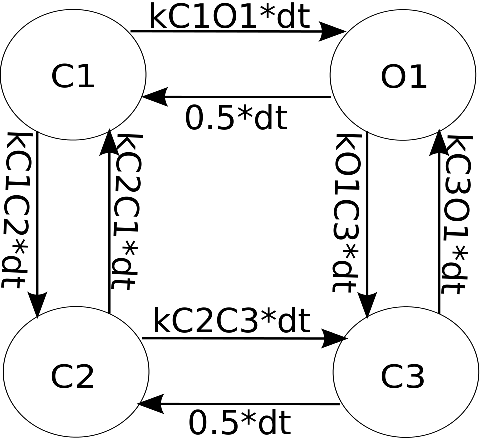
\includegraphics[scale=0.5]{figs/state.pdf}
\caption{The eight possible transitions between four states of a RyR, where the labels on the arrows indicate the
probabilities of the transitions.}
\label{ryrstates}
\end{figure}

在每个细胞里,有约$10000$个钙离子释放单元也叫dyads,这些钙离子释放单元按照$100\times 10\times 10$的三维网格进行排列。每个dyad包含五个不同的小单元,钙离子会在这些小单元里停留,详细的公式和参数可以参考文献\upcite{gaur2011multiscale}。每个dyad空间里,包含15个L-型钙离子通道和$100$个RyRs,它们是随机地活动的。在任何时刻,每个RyR会处于四个状态中的一个,这四个状态用C1、~C2、~C3以及~O1表示。图\ref{ryrstates}中给出了各个状态间可能的转换关系,以及状态间转换的概率,图\ref{ryrstates}状态转换的概率参数是与每个RyR内的钙离子浓度相关的,除了其中从~O1到~C1以及从~C3到~C2的转换概率为常数。处于打开状态(即处于~O1状态)的RyR的个数直接影响到钙离子的流量,进而影响每个细胞内的电压。

dyad中的钙离子浓度可以通过公式\ref{eq:1}至公式\ref{eq:10}来求解。

{
\allowdisplaybreaks
 \begin{eqnarray}
  ca_{\mathrm{ds}}& = & (J_{\mathrm{rel}} + J_{\mathrm{lca}} + ca_{\mathrm{ss}} / \tau_{\mathrm{efflux}})\times \tau_{\mathrm{efflux}}\label{eq:1}\\
  \frac{d\, ca_{\mathrm{ss}}}{dt}& = & \overline{B_{\mathrm{ss}}}\left(  J_{\mathrm{NCX}} + J_{\mathrm{diff\_myo\_ss}} + J_{\mathrm{diff\_ds\_ss}}\right) \label{eq:2}\\
  \frac{d\,ca_{\mathrm{JSR}}}{dt}& = & \overline{B_{\mathrm{JSR}}}\left(J_{\mathrm{rel}} + J_{\mathrm{diff\_NSR\_JSR}}\right) \label{eq:3}\\
  \frac{d\,ca_{\mathrm{NSR}}}{dt}& = & J_{\mathrm{up}} - J_{\mathrm{leak}} - J_{\mathrm{diff\_NSR\_JSR}}  \label{eq:4}\\ 
  \frac{d\,ca_{\mathrm{myo}}}{dt}& = & \overline{B_{\mathrm{myo}}}\left(J_{\mathrm{cab}} + J_{\mathrm{pca}} + J_{\mathrm{NCX}} - J_{\mathrm{up}} + J_{\mathrm{leak}} - J_{\mathrm{diff\_myo\_ss}}\right) \label{eq:5}\\
  Ca_{\mathrm{ds}}& = & (J_{\mathrm{rel}} + J_{\mathrm{lca}} + Ca_{\mathrm{ss}} / \tau_{\mathrm{efflux}})\times \tau_{\mathrm{efflux}}\label{eq:6}\\  
  \frac{\partial Ca_{\mathrm{ss}}}{\partial t}& = & \overline{B_{\mathrm{ss}}} \left(J_{\mathrm{NCX}} + J_{\mathrm{diff\_myo\_ss}} + J_{\mathrm{diff\_ds\_ss}}
+ D_{Ca}\nabla^2Ca_{\mathrm{ss}}\right) \label{eq:7}\\
  \frac{d\,Ca_{\mathrm{JSR}}}{dt}& = & \overline{B_{\mathrm{JSR}}}\left(J_{\mathrm{rel}} + J_{\mathrm{diff\_NSR\_JSR}}\right) \label{eq:8}\\
  \frac{\partial Ca_{\mathrm{NSR}}}{\partial t}& = & J_{\mathrm{up}} - J_{\mathrm{leak}} - J_{\mathrm{diff\_NSR\_JSR}}  +  D_{\mathrm{SR}}\nabla^2 Ca_{\mathrm{NSR}}\label{eq:9}\\					
  \frac{\partial Ca_{\mathrm{myo}}}{\partial t}& = &
                                                     \overline{B_\mathrm{myo}}\left(J_\mathrm{cab} + J_\mathrm{pca} + J_\mathrm{NCX} - J_\mathrm{up} + J_\mathrm{leak} - J_\mathrm{diff\_myo\_ss}\right.\nonumber\\
&&+ \left. D_{Ca}\nabla^2Ca_{\mathrm{myo}}\right)
\label{eq:10}
  \end{eqnarray}
}
%
%\noindent

公式中,$J_{\mathrm{rel}}$是从RyRs到dyad单元间的钙离子流通量,$J_{\mathrm{lca}}$是从L-型钙离子通道到dyad间的钙离子流通量,$\tau_{\mathrm{efflux}}$是dyad空间和膜下空间之间的扩散系数,$J_{\mathrm{NCX}}$是钠离子和钙离子交换在膜下空间产生的电流通量,$J_{\mathrm{diff\_myo\_ss}}$是肌质与膜下空间之间的扩撒流通量,$J_{\mathrm{diff\_ds\_ss}}$是dyad与膜下空间之间的扩撒流通量。$J_{\mathrm{diff\_NSR\_JSR}}$是NSR和JSR间的扩撒流通量,SR泵可以将钙离子从NSR抽到SR中,产生的流通量用$J_{\mathrm{leak}}$来表示。$J_{\mathrm{pca}}$是流过胞质膜的钙离子流通量,膜下空间会被SR和SL瞬间缓冲,瞬间缓冲系数是通过$\overline{B_{\mathrm{ss}}}$来表示的。$\overline{B_{\mathrm{JSR}}}$是CSQN到JSR间的瞬间缓冲系数,$\overline{B_{\mathrm{myo}}}$是从CMDN和TRPN到胞质膜的瞬间缓冲系数。更加详细的关于各个参数和变量的信息可以参考文献\upcite{gaur2011multiscale}。

\subsection{数值策略}
本课题采用随机的方法对L-型钙离子通道和RyRs进行随机模拟,详细的介绍将在\ref{cellImp}中介绍。显式时间积分法被用来求解所有的微分方程(\ref{tissuevoltage})-(\ref{eq:10})。涉及的扩撒项采用中心有限差分的方法进行离散化。而对于单域方程(\ref{tissuevoltage}),使用的是算子分裂方法\upcite{qu1999advanced}。这意味着扩撒项与离子产生的电流项$I_\mathrm{ion}$是分开处理的,后者是通过求解Ord模型中的所有常微分方程得到所有的离子电流,并将所有的离子电流累加起来而得到。

所有的计算流程是发生在一个时间循环内,循环中是每个时间步需要完成的工作,具体包括对所有细胞内的模拟,然后是根据公式\ref{tissuevoltage}对细胞间电压扩撒过程进行计算。每个细胞内的计算包括对所有的dyads进行计算,然后对dyad间的扩撒过程进行计算。具体过程如表\ref{overview}中的伪代码所示,对其中的计算进行高效实现变得非常重要。

\begin{table}
\caption{3D组织模拟计算的伪代码实现}
\label{overview}
\begin{lstlisting}[language=C++, basicstyle=\ttfamily\footnotesize]
Global initialization
  for (int t = 0; t < time steps; t++) {	
    for (int k = 1; k <= cells; k++) {
      Cell computation
      for (int j = 1; j <= dyads; j++) {
        L-type probability calculation
        L-type opening	
        RyR probability calculation
        RyR opening
        Ca concentration computation }
      Dyad diffusion }
    Cell difusion }
\end{lstlisting}
\end{table}

\section{基于多核CPU系统的心脏组织3D模拟的实现}

 \subsection{多级并行}

在介绍大规模心脏组织模拟的实现之前,先介绍实现所面向的目标平台以及相应的编程模型。本课题面向的是多核CPU集群系统,集群中节点间通过以太网或者光纤高速互联,节点间通信可以通过MPI实现,在单节点内也可以创建多个MPI进程进行通信。本课题采用了MPI进行编程,每个MPI进程控制一个计算节点,节点间通过MPI进程进行通信,这种编程方式可移植性好,方便程序员显式控制通信。对于单节点内部来说,每个节点都是由多核CPU构成的,为了充分利用多核CPU的计算资源,本课题采用OpenMP的编程方法,为每一个CPU核分配相应的任务。对于其中的CPU核来说,由于CPU支持向量化执行,因此,还可以进一步利用硬件的并行计算资源。

基于现有的目标平台以及编程模型,本课题采用了一种多级并行策略对大规模心脏组织的模拟进行加速。首先是将3D心脏组织网格划分成很多子网格,每一个网格中的所有细胞的模拟分配给一个计算节点完成,而对于网格中的所有细胞的模拟,由于各个细胞的模拟是相互独立的过程,因此可以采用OpenMP对细胞的模拟并行执行。MPI通信只发生在组织层,因为在计算扩散项\ref{tissuevoltage}时,当前细胞的电压与相邻的细胞的电压有关,这就会涉及到MPI通信了。然而主要的计算还是发生在细胞内, \label{cellImp}将重点介绍单个细胞内的计算的实现。
 
 \subsection{单个细胞内的数值计算实现}
 \label{cellImp}
 在细胞内的所有计算中,最耗时的计算部分是关于钙离子处理的那部分。因此,本节重点关注这部分计算,暂且将这部分计算命名为{\tt computeCalciumInDyad},表\ref{cellfunction}中展示的是该部分计算的伪代码。
 
 \begin{table}
\caption{The function that implements calcium handling per cell.}
\label{cellfunction}
\begin{lstlisting}[language=C++, basicstyle=\ttfamily\footnotesize]
void computeCalciumInDyad()
    {
        generateRandData();
        for(int i=0;i<Ndyads;i++) {
            computateLocalLtypeCurrent();
            computeLocalSRCaRelease();
            computeLocalCaConcentration();
        }
        computeCaConcentrationDiffusion();
    }
\end{lstlisting}
\end{table}

 函数{\tt  computeCalciumInDyad}的计算复杂性直接与dyads的数目成正比,还可以看到函数{\tt  computeCalciumInDyad}中调用了五个函数,其中函数{\tt generateRandData}负责产生大量的随机数,每个时间迭代步中都需要重新产生新的随机数,这些随机数在细胞内L-通道的开和关的模拟中被使用到。函数{\tt  computeCaConcentrationDiffusion}是用来计算细胞内dyad间钙离子扩散中的浓度变化。另外三个函数将在一个{\tt for}循环中调用,特别的,函数{\tt computeLocalSRCaRelease}中的主要部分是计算每个dyad内$100$个RyRs状态间的随机转换过程。在接下来的内容中,将展现三个对并行模拟器性能产生影响的编程和数值技术。
 
 \subsubsection{避免重复计算}
在每个dyad的计算中,都需要计算大量的变量,有些变量在不同的dyad内值是不一样的,因此,对于这些变量,每一个dyad发生的计算中都应该包含这些变量的计算。然而,对于有些变量,其值对于所有的dyad都是相同的,由于dyad数量最多可以达到$10000$,,如果在进入对dyad的{\tt for}循环之前,预先将这些在每一次时间迭代步内不会改变的变量的值计算出来,可以大大减少计算的次数。这需要从这些复杂的公式中找出循环常量,根据实验的性能提升可以发现这些努力是值得的。

\subsubsection{细胞内的dyad间扩散的向量化}
细胞内的$10000$ 个dyads形成一个$100\times10\times10$的网格,钙离子由于浓度不同会在这些dyad间扩散。表\ref{diffusion}中的伪代码是这种3D扩散的计算实现过程,代码主要由三个{\tt for}循环构成,其中计算主要集中在最内的循环,最内的循环次数为$100$,因此可以考虑对该循环进一步优化。由于CPU核已经在细胞级采用OpenMP并行了,每个CPU核负责细胞内的计算,如果需要对细胞内的计算进一步并行,只能开发CPU核内的并行计算资源了。本课题采用的是Intel CPU,每个CPU核内具有256位的向量计算单元,所以对于64位双精度浮点计算来说,每个CPU一次可以处理4个双精度的浮点运算。由于dyad内的数据在$x$方向连续存储的,最内循环适合进行向量化。本课题通过添加编译指导语句,借助编译器对特定的循环进行向量化优化。理论上应该可以取得4倍的加速,但由于扩散中的计算是存储受限的计算,实际取得的性能提升将远低于理论上能取得的性能。

 \begin{table}
\caption{Pragma guided vectorization (in the $x$ direciton) of one of three diffusion computations between the dyads in function {\tt computeCaConcentrationDiffusion}.}
\label{diffusion}
\begin{lstlisting}[language=C++, basicstyle=\ttfamily\footnotesize]
for(z=1;z<Nz_diff-1;z++)
        for(y=1;y<Ny_diff-1;y++) {     
           int x,c,n,s,b,t;         
           x=0;
           c=x+y*Nx_diff+z*Nx_diff*Ny_diff;
           n=c-Nx_diff;            s=c+Nx_diff;
           b=c-Nx_diff*Ny_diff;    t=c+Nx_diff*Ny_diff; 
           
           U[c]=u[c]+fx*(2*u[c+1]-2*u[c])+fy*(u[n]+u[s]-2*u[c])
                    +fz*(u[b]+u[t]-2*u[c]);
           #pragma ivdep
           for(x=1;x<Nx_diff-1;x++) {
              ++c; ++n; ++s; ++b; ++t;
              U[c]=u[c]+fx*(u[c-1]+u[c+1]-2*u[c])+fy*(u[n]+u[s]-2*u[c])
                       +fz*(u[b]+u[t]-2*u[c]);              
           }
           U[c]=u[c]+fx*(2*u[c-1]-2*u[c])+fy*(u[n]+u[s]-2*u[c])
                                         +fz*(u[b]+u[t]-2*u[c]);
        }   \end{lstlisting}
\end{table}


\subsubsection{采用二项分布}
\label{binom}
%
前面的章节中已经介绍了每个dyad内包含$100$ RyRs,每个RyR在任何时刻会处于四种状态中的一种状态,在\ref{cellmodel}已经介绍了这四种状态,以及这四种状态间的转变关系,状态间的转变是按照一定的概率随机转变的。现在的目标是计算RyR中处于打开状态(O1)的数目,因为打开状态的RyR能够决定钙离子流量而影响细胞内电压,一种直接的方法是对每个RyR独立地进行模拟。这样每个dyad内需要消耗100个随机数对这100个RyRs的状态转变进行模拟。每个RyR根据当前状态以及相关的转变概率转变到另一个状态中,这种模拟的方法需要消耗大量的计算,一方面是因为需要消耗大量的随机数,随机数在每个时间步中都需要重新产生;另一方面,这种模拟实现中,代码含有大量的{\tt if}测试语句。

因此,如果能将dyad内的100个RyRs看作一个整体,直接计算出处于开放状态的RyR的数目,将有效降低计算量。因此,本课题将原本100次独立的随机试验替换为在一个二项分布中进行八次随机抽样的实验,对图\ref{ryrstates}中的每一次转变进行一次抽样试验。在二项分布中,$n$次试验中成功$k$次的概率为$p$,则$p$可以用公式\ref{eq:cumulative}计算。

\begin{equation}
F(k,n,p)=Pr({X}\leq{k})=\sum_{i=0}^{k}\binom{n}{i}p^i(1-p)^{n-i},
\label{eq:cumulative}
\end{equation}
式中$$\binom{n}{i}=\frac{n!}{i!(n-i)!}$$为二项系数。由于处于各个状态的RyRs的数目是从$0$ 到$100$间变化,可以预先计算好所有的二项系数,这也能显著提高计算性能。

使用服从$[0,1]$的均匀分布的随机数,对二项分布进行采样找出最小的$k$,使得$r \leq F(k,n,p)$。然而标准的二项分布实现对计算需求比较大,本课题采用了一个高效的实现,如表\ref{fig:binom}中代码所示。因为二项分布的系数预先已经计算出来了,只需要在每一轮试验中将$p/(1-p)$与基概率$(1-p)^n$相乘,并与二项系数相乘然后保存结果。

 \begin{table}
\caption{Implementation of Binomial Distribution Method. Function {\tt constant\_p\_binomial} simply finds $k$ by using the precomputed lookup table. In function {\tt binomial},
we first test if the computation can be skipped, using the threshold $p_t$ and the precomputed value $F(0,n,p_t)$. If this is not the case, the distribution function $F(k,n,p)$ is computed iteratively by subtracting from {\tt randValue} using the precomputed binomial coefficients.}
\label{fig:binom}
\begin{lstlisting}[language=C++, basicstyle=\ttfamily\footnotesize]
    int constant_p_binomial(n,randValue) {
        k=0;
        while(randValue>Table[n,k]) 
            k++;
        return k;
    }

    int binomial(n,p,randValue) {
        	if n = 0
		    return 0;
        if p < Threshold AND randValue < Precomp[n]
            return 0;
        k = 0;
        p_current =pow((1-p),n);
        p_step = p/(1-p);
        while(randValue > 0) {
            k++;
            randValue -= Binom[n,k]*p_current;
            p_current *= p_step;
        }
        return k;
    }  
           \end{lstlisting}
\end{table}

为了表示方便,用$x_1$,$x_2$,$x_3$,$x_4$这四个变量代表RyR处在四种状态的数目,并用$x_{ij}$表示RyR从状态$i$到状态$j$间的数目,$x_{ij}$是通过上述描述的方法通过对二项分布采用计算出来的。因此,在下一个时间步,处于各个状态的RyR数目可以用公式\ref{transitNumber}计算。

\begin{equation}
\label{transitNumber}
x_i = x_i - \sum_{j}x_{ij}+\sum_{j}x_{ji}.
\end{equation}

基于此,本课题根据细胞模型的特点增加了两个优化方法,在本课题中提出的细胞模型中,RyR中的状态中,从O1到C1和从C3到C2的转化概率为常数,即$p_c=0.5*dt$。因此,可以仿照预先计算二项系数的思路,也预先计算全部的累积概率函数$F(k,n,p_c)$。在这两种方法中,唯一的代价是需要存储$101*100/2=5050$个双精度浮点值,这增加了一些额外的存储开销。

另外,本课题还利用了细胞模型中另一个特性,就是RyR中大部分时间都是处于C2状态的,并且状态间的转变概率除了上述所说的两个为常数概率,其它转变概率在大部分时间都是接近0的。这意味着通过从二项分布中采样计算出的转变的RyR的数目也接近0。本课题通过设置一个小的概率阈值记为 $p_t$,并且对于所有的$0 \leq n \leq 100$,预先计算出$F(0,n,p_t)$ 。如果$p \leq p_t$,只要检查随机数$r$,看是否满足$r \leq F(0,n,p_t)$,如果满足,则$k=0$,代表没有发生状态转变,就可以不用计算二项分布了。当然,如果转变前处在某个状态的RyR数为0,那么发生状态转变的RyR数也为0,详细的代码参见表\ref{fig:binom}.

采用二项分布对RyR状态转变进行模拟的方法也在文献\upcite{restrepo2008calsequestrin}中被采用了,然而作者并没有去计算实际的二项分布,而是采用正态分布和泊松分布对其进行逼近,不过这会降低模拟的精度。
   
   
\section{实验结果与分析}
\subsection{实验设置}

本课题的测试系统是在Abel\upcite{abel}机器上,这是一个由奥斯陆大学管理维护的一个超级计算机系统。在Abel机器上的每个计算节点由Intel Xeon E5-2670处理器构成,共有16个物理计算核心,每个计算核心的频率为2.6GHz,由FDR Infiniband互联(56 Gbps)。本课题最多使用了128个计算节点(即2048个CPU核)进行数值模拟试验。本课题采用Intel的\textit{icc} 15.1.0编译器,Intel MPI 5.0.2库进行通信。

在所有的试验中,无论是组织层级还是细胞层级都采用大小为$0.05$ ms的固定的时间步。在组织层级模拟中,对于公式\ref{tissuevoltage}中扩散项的离散化,本课题选择了$0.5$ mm的固定的网格分辨率。

\subsection{性能优化实验}
第一个数值计算的试验是为了测试\ref{cellImp}中在函数{\tt compute\_cell}中介绍的那些优化方法的性能提升效果。为了测试这些优化方法的性能,对包含$10000$个dyad的细胞模拟$10000$个时间步,等价于模拟一次持续时间为$500$ ms的心脏跳动。模拟期间,在$t=50$时刻给细胞一次刺激。图\ref{fig:optimizations}给出了各个不同的优化方法的性能提升。通过避免重复计算可以显著提高各个函数的性能,其中函数{\tt computateLocalLtypeCurrent}的性能提升$37.5\%$,函数{\tt computeLocalSRCaRelease}的性能提升$24.4\%$,函数{\tt computeCaConcentrationDiffusion}的性能提升$12.4\%$。向量化能进一步加速扩散部分的计算,加速约$25\%$。最后是采用二项分布的方法对RyR通道的模拟的影响,从试验结果看,二项分布方法对性能影响最大,能过加速SRCaRelease约$70\%$,在随机数产生方面可以提升$79.9\%$,对于后者的影响完全是因为二项分布的方法可以有效减少对随机数的使用。最后,在所有的方法都使用后,总的时间减少了约$50.7\%$。

\begin{figure}[htb]
\center
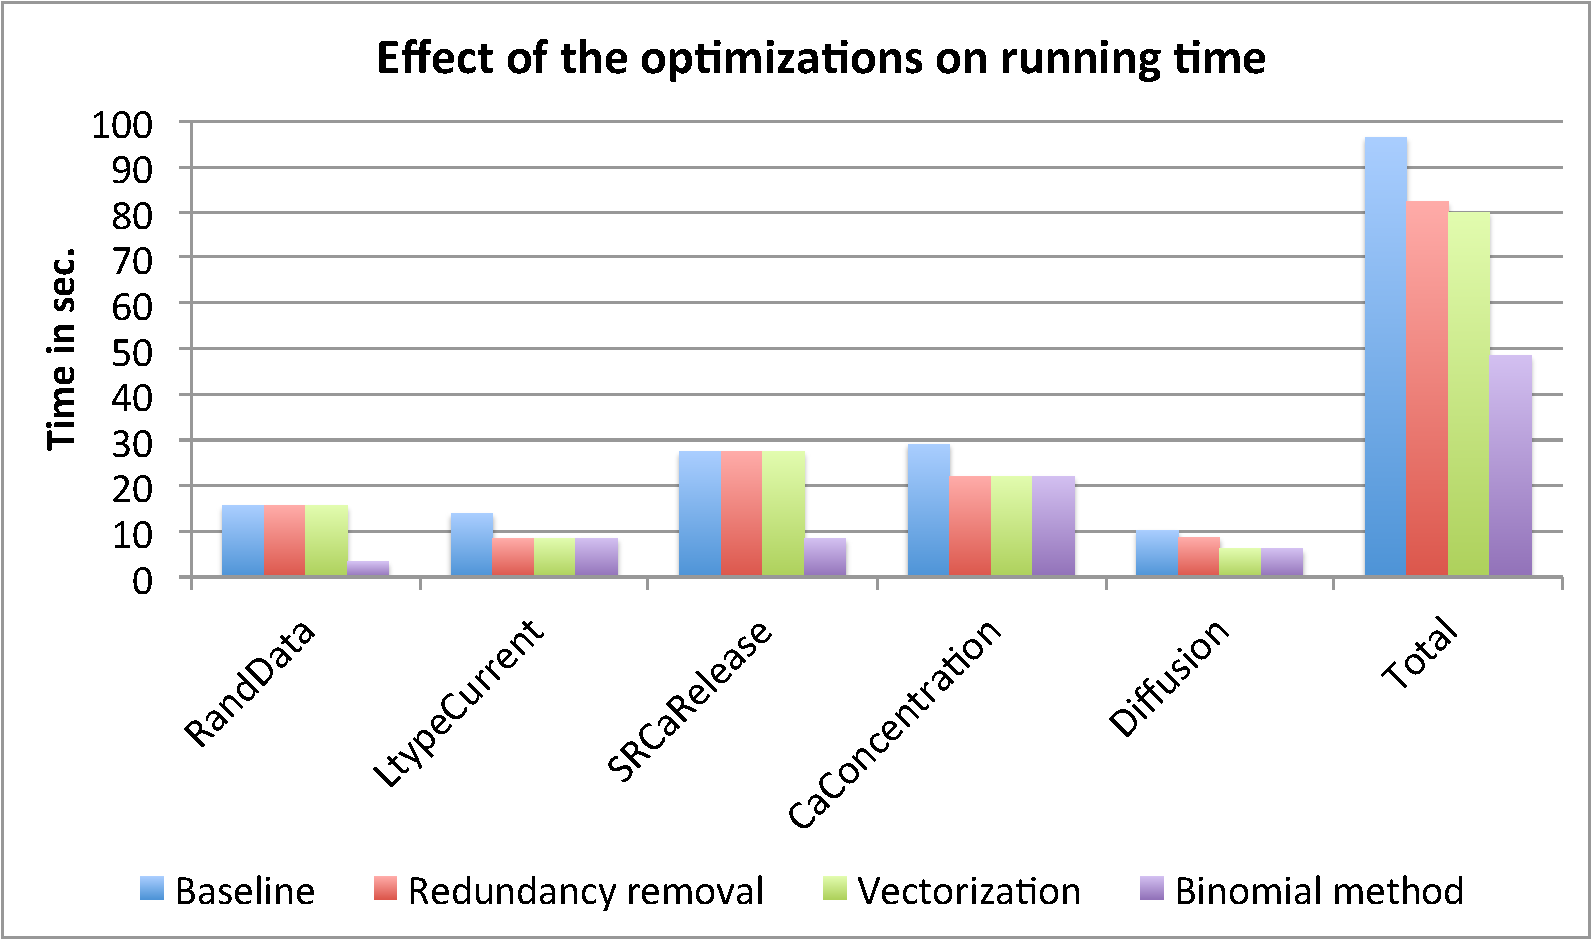
\includegraphics[width=\textwidth]{figs/optimization.pdf}
\caption{Performance improvement of the individual functions in {\tt computeCalciumInDyad} due to the different optimization techniques. The three optimizations are applied cumulatively. Thus, the values for the Binominal method reflect the sum of all improvements.}
\label{fig:optimizations}
\end{figure} 

\subsection{扩展性实验}
本章对弱扩展和强扩展都进行了试验,试验中模拟时长为$1000$ ms,对于两个扩展试验,分别都做了两个模拟试验,一个是细胞内的dyad数量设置为$100$个,另一个是细胞内dyad数量设置为$10000$。

在弱扩展试验中,本课题使用的计算节点的数目从$1$到$128$。当使用$100$个dyad时,为每个计算节点分配的心脏组织大小为$64\times64\times64$,$128$个计算节点上完成大小为$512\times256\times256$ 的心脏组织的模拟。对于$10000$个dyad来说,为每个计算节点分配的心脏组织大小为$16\times16\times16$,$128$个节点分配心脏组织大小为$128\times64\times64$。扩展性试验中,每秒钟能够完成的细胞计算量作为扩展性的衡量标准,一个细胞计算量是指一个时间步计算一个细胞。图\ref{scaling}给出了弱扩展试验的结果,其中纵坐标代表细胞计算量,横坐标是使用的计算节点数。从结果看出,试验表现出很好的弱扩展性。

对于强扩展试验中细胞内dyad设置为$100$个时,心脏组织大小固定在$256\times256\times256$这个规模,而对于每个细胞内dyad数量为$10000$,心脏组织规模为$32\times32\times32$,由于存储的需求,强扩展试验中最少需要$8$ 个计算节点。与弱扩展试验中类似,仍然采用细胞计算量这个指标,图\ref{scaling}也展示了强扩展试验的结果。强扩展基本上取得了与弱扩展一样的性能。性能上细微的差别可以通过通信量来解释,强扩展试验中通信量会比弱扩展试验大些,而在现有的实现中,通信暂且未做优化。

由于心脏细胞模拟是计算密集型的应用,因此,无论是在弱扩展,还是强扩展试验中,模拟试验都表现了很好的扩展性。通过每秒细胞计算量这个指标,可以对任何规模的心脏组织在给定计算资源的条件下需要模拟的时间进行预测。

\begin{figure}[htb]
\center
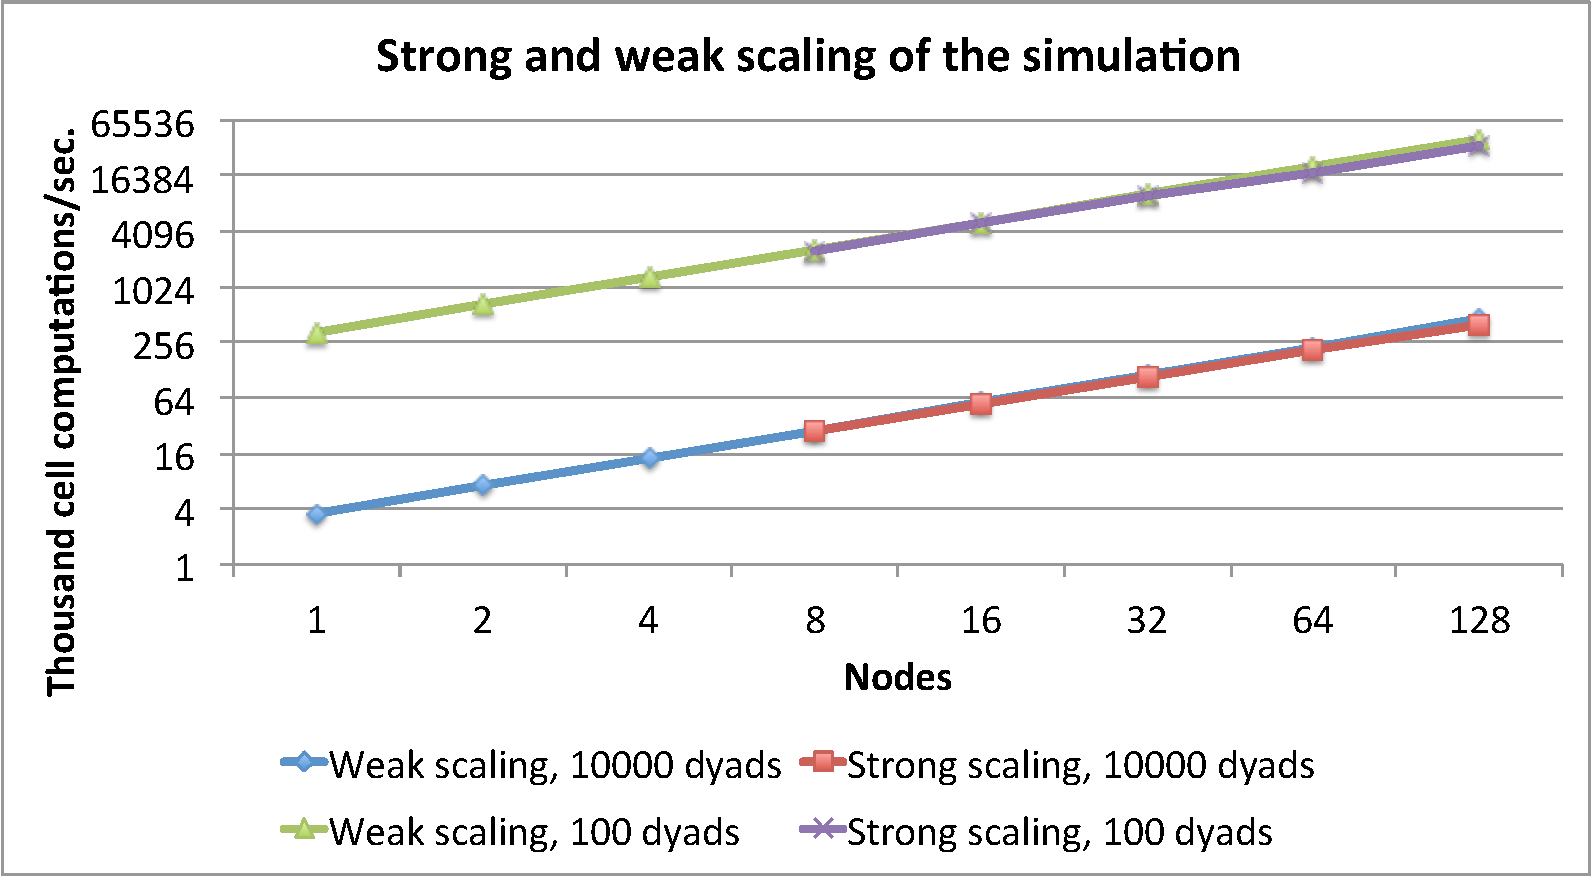
\includegraphics[width=\textwidth]{figs/scaling.pdf}
\label{scaling}
\caption{Performance of weak and strong scaling tests of tissue simulations. The $Y$ axis shows performance measured via the number of cell computations (i.e.~time steps for a single cell) performed for each wall-clock second of simulation time used. }
\end{figure} 


\subsection{细胞内离子活动实验}

\begin{figure}[htb]
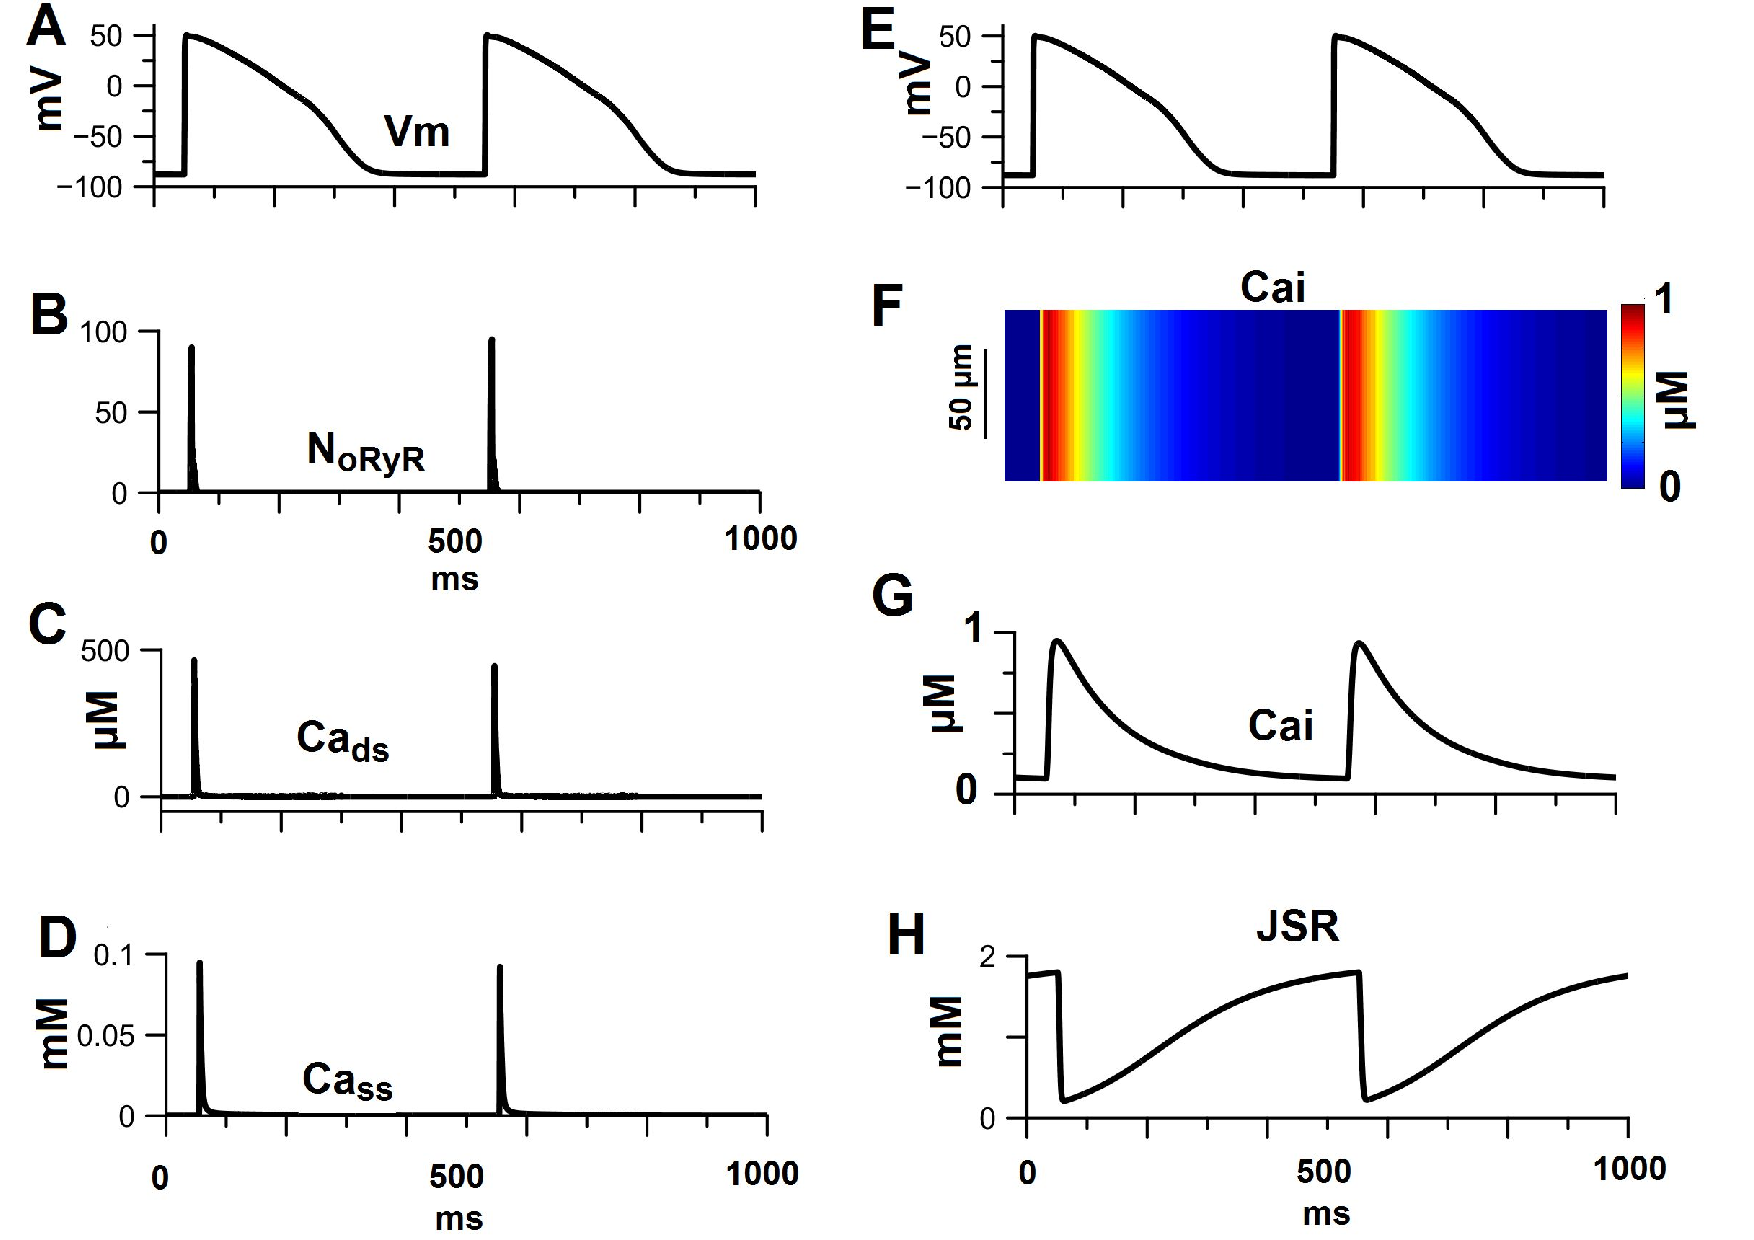
\includegraphics[width=\textwidth]{figs/calcium.pdf}
\caption{Calcium handling in a cell in a human tissue during normal excitation. (A) Action Potential. (B) Number of open RyRs ($N_oRyR$) in the center dyad of the cell. (C) Dyadic space calcium ($Ca_{ds}$) (D) Submembrane space calcium ($Ca_{ss}$) (F) Simulated linescan image of intracellular Ca ($Ca_i$ (G) Whole-cell $Ca_i$ and (H) Whole-cell junctional sarcoplasmic reticulum (JSR). The 3D tissue was plane-stimulated at an edge at a cycle length(CL)=500 ms. Last two steady-state beats are shown.}
\label{fig:calciumcell}
\end{figure}

在图\ref{fig:calciumcell}中,我们展示了人类心脏细胞内正常的心跳过程中钙离子处理变化过程。试验以不同的尺度展示了心脏组织的中心细胞内钙离子处理结果。图\ref{fig:calciumcell}中A部分显示了在两次连续的心脏中活动电势的变化;图\ref{fig:calciumcell}中B部分是位于细胞中心的dyad内处于打开状态的RyR的数目,这些数目是按照\ref{binom}通过二项分布的方法计算出来的。模拟结果表明,在活动电势变化期间,大部分RyR是出于打开状态的,随着这些通道的打开,在dyad内的$Ca_{ds}$浓度迅速上升到$500\mu$M,以及$Ca_{ss}$上升到$0.1$mM,具体变换过程可以从图\ref{fig:calciumcell}中的C和D观察到。对于亚细胞层级,对细胞内的Ca ($Ca_{i}$)进行模拟的线扫描影像表明,细胞内所有dyad内的钙离子释放是同步发生的(参考图\ref{fig:calciumcell}的F)。整个细胞内相关的$Ca_i$为图\ref{fig:calciumcell}中G所示,以及H未整个细胞的JSR。总之,这些结果描述了正常心脏跳动过程中的不同尺度的钙离子处理过程,包括dyad级、亚细胞级以及细胞级。

\subsection{心脏组织内异常活动模拟}

图\ref{arrhythmia}在3D心脏组织中的膜电位变化图,在时刻t = 0 ms,心脏组织的边缘受到一个刺激,经过一段时间的电压传播,在t = 600 ms时,心脏组织的一部分细胞受到新的刺激,在新刺激和之前的电压扩散的双重影响下,最后在心脏组织内部形成一个卷波。从心脏组织中的三个位置A、B、C的细胞进行采样,这三个位置的膜电位变化如图\ref{arrhythmia}中下半部分所示。在整个模拟过程中,卷波非常稳定,没有产生新的小波。这个模拟试验表明了本课题实现的这个组织模拟器能够模拟出在心脏组织的异常功能研究中非常有用的卷波。

\begin{figure}[htbp]
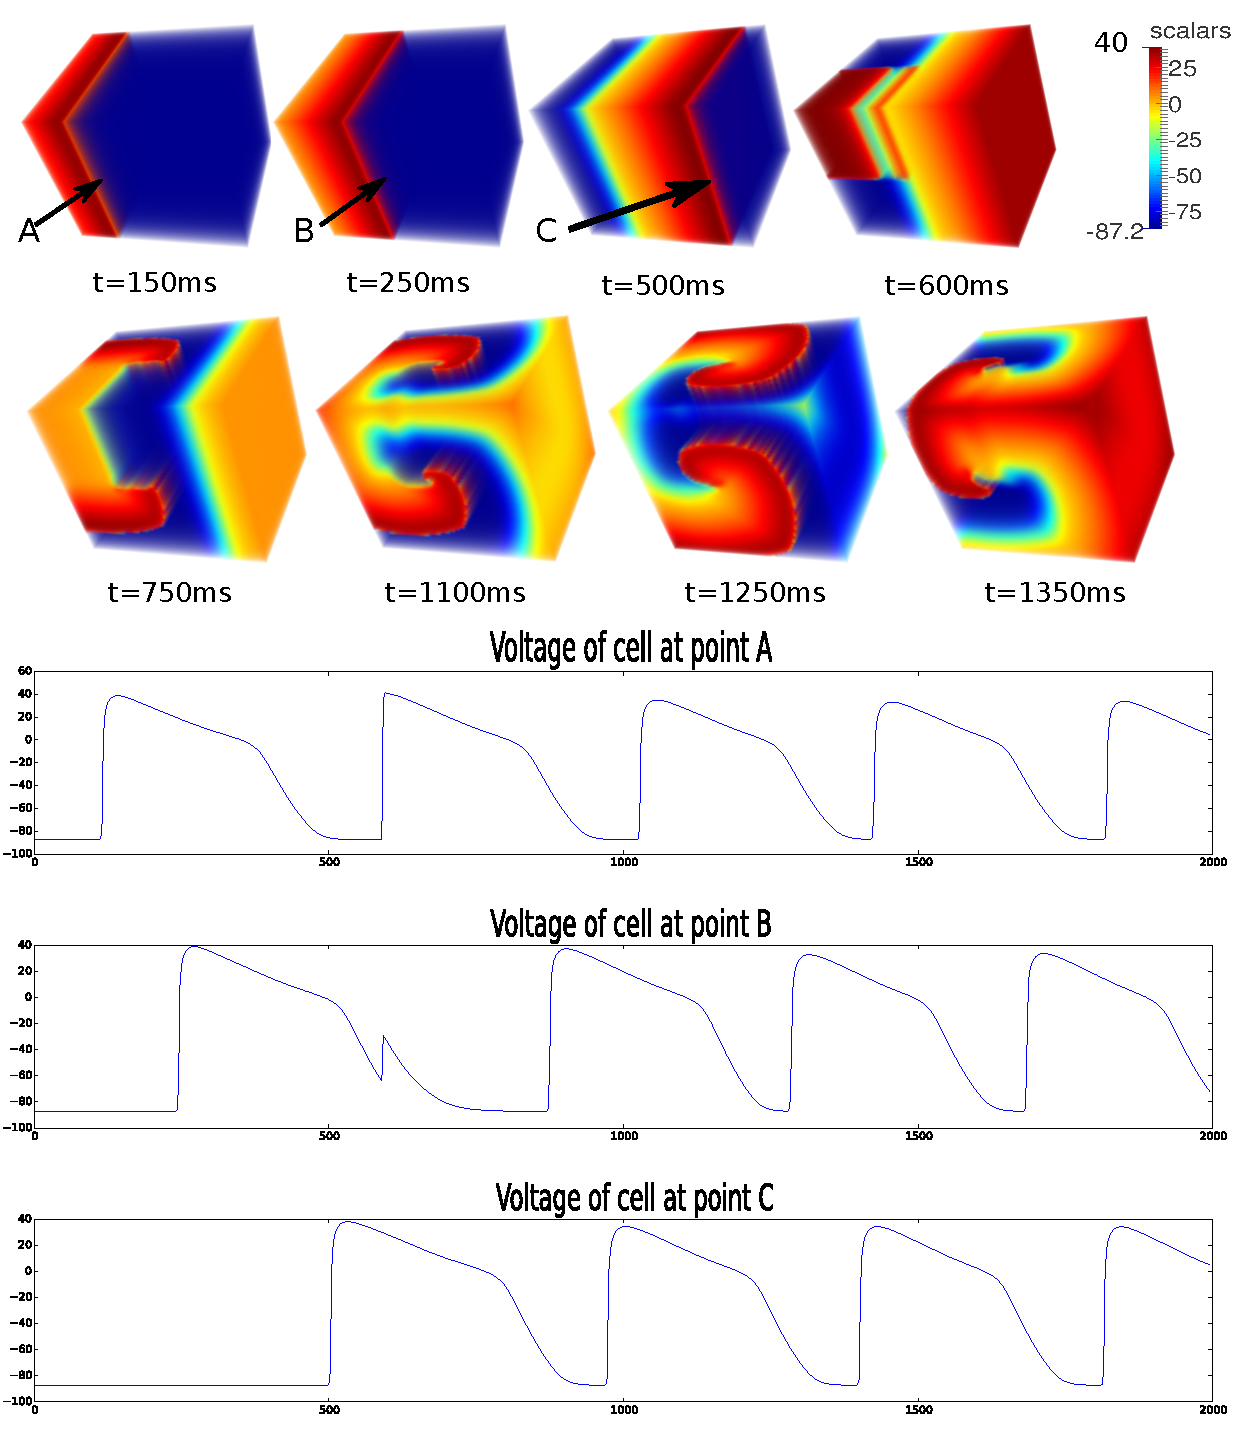
\includegraphics[width=\textwidth]{figs/voltage}
\caption{Simulation of scroll waves in a 3D tissue. The top part shows voltage snapshots at different time points. The bottom section shows membrane potentials at three different locations in the tissue.}
\label{arrhythmia}
\end{figure}

\section{小结}
本章介绍了3D组织模拟的精细模型,采用了细胞内多尺度钙离子处理模型对心脏组织细胞的电活动和钙离子处理过程进行模拟。以往针对3D心脏组织的许多研究都是利用全细胞钙离子处理模型,而多尺度的钙离子处理模型并没有在组织模拟中广泛使用,其中的原因一方面是因为多尺度模型模拟对计算需求巨大;另一方面是当今缺少针对这些计算的有效的数值方法和算法。而本课题提出了一个多尺度模拟的模型,并在大规模的集群系统实现了。在实现过程中,本课题采用了多种优化方法,首先是减少了心脏组织细胞的模型中的很多变量的重复计算,其次是根据硬件平台的并行计算资源对3D心脏组织进行了多级并行,最后对心脏组织模拟的核心模拟过程采用了二项分布的方法。这些优化方法使得模拟的时间减少了一半。对性能提升效果最明显的是二项分布方法的引入,二项分布方法减少了对随机数的使用,可以节省大量用于产生随机数的时间。

弱扩展测试针对不同的组织规模,在不同数目的计算节点上基本保持了相同的计算时间。而强扩展试验中,随着计算节点数目的增加,计算时间基本保持了一个线性下降的关系。这些结果表明了将更大规模的心脏组织模拟映射到更大规模的集群系统中进行模拟成为可能。最后通过试验证明了本课题研究针对心脏组织细胞内的钙离子处理模拟与已经发表的工作\upcite{o2011simulation}的结论是一致的。试验也证明了本课题研究的模型能够模拟3D心脏组织的心率失常等问题。

总结本章工作,本章提出了一个精细的3D心脏组织模拟模型,这个模型能够模拟人类心脏组织细胞内的电活动和钙离子处理过程,通过采用多个优化方法,最后将模型在大规模多核系统高效地实现了。试验中的扩展性结果表明全心脏的模拟在当前最快的超级计算上进行模拟也是可能的。在下一章中,本课题将进一步提高3D组织模拟器的性能,并且将已有的实现移植到更快的硬件加速器系统中。这将逐渐从多个尺度增加研究人员对心脏病理的机制的理解。





\chapter{心脏组织模拟在天河2异构系统上的并行优化}
\label{icpads}

\section{引言}
在\ref{ICA3PP}中,已经介绍了心脏组织模拟在研究心律失常等各种心脏疾病具有重要的作用,心脏组织模拟的模型越详细,对计算的需求越大,在\ref{ICA3PP}中也已经介绍了本课题在多核CPU的集群系统上做的一些工作,采用了MPI+OpenMP的并行编程方法,对一定规模的心脏组织进行了模拟。但如果想对更大规模的心脏组织模拟则需要计算能力更强的处理器或者加速器构成的超大规模集群系统。文献中\upcite{GPUcell}采用了GPU在细胞层级对模拟进行加速,利用加速器对模拟进行加速不失为一种好的选择。

基于现有的计算资源,本课题将心脏组织模拟移植到超级异构集群系统即天河2号超级计算机\upcite{tianhe}上。天河2号超级计算机系统在TOP500排名中位居第二,它的每个计算节点都是由Intel CPU与Intel PHI协处理器构成的异构系统。

众核加速器的每个芯片集成了大量的简单小核,非常适合作为高性能计算系统的核心计算部件。Intel的Xeon Phi协处理器和GPU是两种典型的众核加速器。本课题将面向天河2号超级计算机系统实现心脏组织的3D模拟,天河2号超级计算机系统采用多核CPU作为控制核心以及Intel Xeon Phi协处理器作为加速部件。天河2号系统的峰值性能可以达到54.9PFlops,实测性能可以达到33.86PFlops。

天河2号系统具有很强的计算能力,但天河2号作为复杂的异构系统,这给天河2号上的并行编程带来了诸多挑战。因此,对于一个应用能否在天河2号上取得很好的性能,取决于并行实现。对于天河2号系统来说,除了需要高效地充分利用其大量的硬件线程,单个物理线程上的SIMD向量化也需要尽可能地得到发挥。物理线程的并行可以通过OpenMP编程实现,或者通过一个MPI进程内创建多个OpenMP线程控制多个物理线程,SIMD向量化理论上能够将双精度的浮点性能提升8倍,SIMD向量化可以在代码中添加编译指导语句,借助编译器对代码自动向量化,或者采用AVX-512向量指令\upcite{XEONPHI}手动对代码进行向量化。编译器自动向量化的方法只针对代码中比较规则的计算,而对于不规则的代码则需要通过手动向量化实现SIMD。

对于由CPU和Xeon Phi构成的异构系统来说,多核CPU的性能同样不容忽略,目前每个计算节点内CPU核的个数一般在8到18之间,然而每个CPU核使用更高的时钟频率,功能也更加强大,更加灵活,适合做一些控制的任务。对于一些特殊的计算,比如很难实现SIMD或者是存储带宽受限,则多核CPU上的实现性能可以达到协处理器上的实现性能。因此异构节点上CPU核与Xeon Phi协处理器应该协同起来,充分发挥异构系统的性能。然而,从编程的角度来说,异构计算可能带来新的问题,比如,对于SIMD向量化,CPU采用不同的AVX指令集,因为CPU的SIMD指令是针对256位的向量计算。异构计算还可能需要解决优化CPU和Xeon Phi间的数据传输问题以及CPU和Xeon Phi间的负载均衡问题等。

本课题的目标是将心脏组织的模拟移植到天河2号的超级异构计算机系统中,为了有效地使用天河2号的硬件资源,需要将模拟的计算过程进行多层次的并行开发,包括计算节点间的并行、节点内CPU和Phi设备间的并行、Phi设备上众核间的并行以及Phi设备的每个计算核心内SIMD的并行。这无疑会给编程带来巨大的挑战,这正是本课题需要解决的问题。

本章内容安排如下,首先将介绍天河2号超级计算机系统的硬件结构;然后将介绍心脏组织模拟在天河2号系统上的高性能并行实现与优化,主要利用硬件结构的特点,将心脏组织模拟的并行映射到具体的硬件中执行,并对其中的关键计算部分进行优化;最后是对试验结果评测,主要测试了心脏组织模拟在天河2号上单节点内的Phi设备上的性能、单节点的性能以及多节点的性能。试验结果表明,本课题针对天河2号异构集群系统开发出了一个高效的心脏组织模拟器。

\section{目标硬件体系结构}

\section{心脏组织模拟的数学建模}


\section{心脏组织模拟的高性能并行实现与优化}

 \subsection{心脏组织模拟的tissue-级并行}
 
 \subsection{心脏组织模拟的cell-级并行}

\subsection{心脏组织模拟的dyad-级并行}

\subsection{心脏组织模拟中随机数生成}


\subsection{代码优化}



\section{实验结果与分析}
\subsection{实验设置}

\subsubsection{心脏组织模拟单设备性能}

\subsection{心脏组织模拟的单节点性能}

\subsection{心脏组织模拟的多节点性能}

\subsection{心脏组织模拟试验}

\section{小结}

%*********************第三章******************
\chapter{3D卷积神经网络在异构平台上的高性能实现}
\label{3DWinograd}
\section{引言}
卷积神经网络在图像分类、目标跟踪等很多2D输入的处理任务已经得到了成功的应用。卷积神经网络能够很好地提取特征,所以卷积网络常用于图像分类,比如Alexnet\ref{}、VGG\ref{} 、googlenet\ref{}、resinet\ref{}等卷积神经网络被用来对2D图像进行分类,达到了很好的分类效果。图\ref{}为经典的Alexnet网络,其主要包含大量的卷积层,其中的计算也主要集中在卷积层。

正因为2D卷积网络得到了广泛的应用,所以研究人员开始转向3D卷积神经网络的研究,在\ref{}已经为我们展现了一个名为ObjectNet3D用于3D物体识别的数据库,通过这个数据库的训练,可以达到识别3D的各种姿势的目的,类似于这样的3D数据库还有ShapeNet\ref{}。针对这些3D数据库的3D卷积网络也开始陆续被设计出来,比如Voxnet\ref{}就是一个用于解决3D物体识别的3D卷积神经网络,文章\ref{}提出用3D卷积神经网络解决人类动作识别的方法,此外, 3D卷积神经网络可以处理视频分类的应用\ref{}。

但对于3D卷积神经网络的应用来说,如果仍然采用2D卷积神经网络的方法来处理,就会存在计算量大,存储消耗大的问题。有些方法只能解决其中的一个问题,比如基于FFT变换的方法在某些情况下可以有效降低计算量,但是以消耗存储为代价的。有一种卷积计算的快速算法,称为WMFA(Winograd Minimal Filtering Algorithm),这种算法目前已经成功运用在2D卷积神经网络中,能够有效降低卷积中的计算量,并且不会增加额外的存储空间。因此,将2D WMFA应用到3D卷积神经网络中是非常值得研究的课题。本章内容主要是介绍3D WMFA算法在3D卷积网络上的应用,需要解决的问题包括,由2D WMFA算法的形式推倒出3D WMFA的形式;从理论上分析3D WMFA算法的复杂性,证明该算法在计算和存储开销上的优势;面向GPU异构平台,将3D WMFA算法高效地映射到GPU上。

本章内容安排如下:第二节介绍了关于卷积神经网络中加速的一些研究现状;第三节介绍快速卷积算法WMFA的3D形式,以及3D WMFA算法的复杂性分析;第四节将重点介绍3D WMFA算法的GPU实现,并且介绍了面向GPU的几种优化技术;第五节将对3D WMFA算法的性能进行评测,并与其它卷积方法的性能进行了对比;最后是对本章内容的总结,随着3D卷积网络应用的推广,对其进行加速变得尤为重要。

\section{相关研究}
对于卷积神经网络的加速,目前主要集中在对2D卷积神经网络的加速研究中,加速的方法主要包括网络结构的改进、算法的改进、深度学习框架中加速库的使用以及新的平台的使用。

Alexnet\ref{}是最早被提出的卷积神经网络,在图像分类应用中,与传统的机器学习分类方法\ref{}相比,分类精度得到大幅度提高,这也开启了对卷积神经网络研究的热潮。为了进一步提高效果,VGG\ref{}网络增加了卷积层的层数(最深多达19层卷积层),这样可以对待分类的图片提取更多的特征,提高分类的精度,虽然所有卷积核大小采用$3\times 3$的卷积核来控制计算量,但由于卷积层数多,计算量仍然很大。Network in Network(NIN)\ref{}是对卷积层的改进,卷积操作是一种线性变换,对特征为线性可分的输入分类效果会很好,而NIN就是解决输入为非线性可分的情况,NIN结构是在卷积层中间引入一个非线性变换操作。GoogleNet\ref{}的设计思路是通过增加网络的深度和宽度来提高分类的精度,但GoogleNet考虑到了计算量的问题,网络结构中引入了很多$1\times 1$的卷积核,该改进可以有效地防止计算量膨胀的问题。 squeezenet\ref{}网络结构在设计上也兼顾了计算量以及模型参数大小两方面,其主要优势就是在保证最后分类精度的情形下减少模型参数。

目前对于比较流行的深度学习框架,比如Caffe\ref{}、Tensorflow\ref{}、Theano\ref{}、Mxnet\ref{}等,它们都采用了专门优化的库实现其中的卷积计算。cblas是面向多核CPU的高效库,cuDNN\ref{}是面向Nvidia GPU的深度学习库。深度学习框架为深度学习开发者提供了一种非常简便的方式来开发深度学习应用,开发者只需要在配置文件中配置使用的平台,就能调用相应的库充分发挥这些底层平台的性能。

现有深度学习框架中调用的库中对卷积的实现大都是将卷积转化为矩阵乘的方法,矩阵分解的方法。。。。还有对卷积计算采用新的等价计算方法,比如FFT的方法\ref{}是将卷积转化为点乘,FFT方法针对卷积核比较大的卷积网络能够显著降低计算量,存在的唯一问题就是存储消耗过大。在卷积算法改进方面的研究还包括本章内容要介绍的应用到3D卷积网络的WMFA方法, Lavin\ref{}在GPU平台高效地实现了WMFA算法,取得了比cuDNN更好的性能。而在文章\ref{}中,作者面向的是FPGA平台,采用OpenCL实现了WMFA算法。无论是GPU平台还是FPGA平台,WMFA算法都表现了很好的并行性。

除了算法方面的改进,也有一些利用集群系统来提高卷积网络的性能。Adam等人开发的COTS HPC系统\ref{}是基于GPU服务器的集群系统,能够对大规模的神经网络进行训练。Google公司使用多年的分布式深度网络框架DistBelief\ref{}使用上千个CPU核心对几十亿的网络参数进行训练。Marthin等人\ref{}对训练的梯度下降法SGD\ref{}提出了一个高效的数据并行算法。H. Wang等人开发的MVAPICH2-GPU\ref{}针对集群中的InfiniBand连接,将CUDA集成在MPICH2中,从而解决了集群系统中的GPU间的通信问题,提高了MPI通信的效率。Mu Li等人\ref{}通过参数服务器的方法提高了在集群上训练的通信效率。

本章的工作主要是借鉴2D卷积网络中算法加速的相关研究,来加速3D卷积神经网络的计算过程。
\section{快速3D卷级算法}




\subsection{3D卷级神经网络定义}

\subsection{3D Winograd 算法}

\subsection{3D Winograd 算法的复杂性分析}


\section{3D Winograd 算法的实现与优化}

\subsection{3D Winograd 算法的实现}

\subsection{3D Winograd 算法的优化}


\section{实验评测与分析}
\subsection{实验设置}


\subsection{3D Winograd 算法各优化方法的性能}


\subsection{3D Winograd 算法各kernel执行时间分布}


\subsection{3D Winograd 算法与其它卷级算法性能比较}


\section{小结}


%*********************第四章******************
\chapter{基于OpenCL的TLD算法高性能实现}
\section{引言}
在前两章中,通过在算法层次上优化当前具有领先精度的跟踪器KCF,以及适用于视觉跟踪的目标候选生成器EdgeBoxes,并将两者有效结合起来,取得了令人满意的视觉跟踪性能。
但是,随着机器视觉应用对精度和鲁棒性的要求不断提高,跟踪器的结构正日趋复杂,计算负载与日俱增,高质量、高性能的跟踪器实现变得越来越关键。
这一点在视觉跟踪领域顶级竞赛VOT(Visual Object Tracking)中也得到了印证。作为第一届VOT竞赛,VOT2013\upcite{vot2013}选取了16个视频序列,每个序列突出一个视觉跟踪中的难点(如遮挡,光照变化等)。首届获胜的跟踪器PLT\upcite{plt}采用二值化特征作为目标描述,并用查找表的方式实现了线性分类器,因此其C++实现达到了169.59 FPS的极高速度。VOT2014\upcite{vot2014}将视频序列扩充为25个,且标记目标物体的矩形框允许旋转,对跟踪器提出了更高难度的挑战。该届获胜的DSST\upcite{dsst}由互相配合的两个相关滤波器构成,一个用于判断目标中心位置,一个用于判断最佳目标大小。结构的简洁性和相关滤波的低计算量使得其Matlab版本也能够做到实时处理(24 FPS)。VOT2015\upcite{vot2015}的视频序列达到了60个,且难度大幅增加。为了应对挑战,MDNet\upcite{mdnet}采用了专门面向视觉跟踪的6层卷积神经网络(CNN),并按照高斯分布大量采样不同位置、不同大小的局部图像进行检测。尽管MDNet在精度和鲁棒性上取得了第一名,但是由于它的计算量很大,实现(Matlab+MatConvNet)又较为粗糙,仅能达到1 FPS的跟踪速度,无法满足实时在线跟踪的要求。

由此可见,在跟踪算法日益复杂的趋势下,为了保证跟踪算法的实用性,或者说为了提高视觉跟踪对计算复杂性的容忍度,研究跟踪算法的高性能实现十分必要。
这里的高性能实现,和``高性能计算''属同一范畴,意指在实现过程中针对硬件体系结构特征,充分发挥计算设备/平台的计算能力。
通过分析体系结构和高性能计算的发展可以看出,并行化无疑是解决高性能实现问题的关键。利用多核并行、向量指令、流水化等并行手段,可以充分发挥通用处理器(CPU)的计算能力。
除了CPU这一经典计算设备,当前包含两类甚至多类计算设备的异构计算平台正方兴未艾。从SoC芯片(如Qualcomm Snapdragon 835\upcite{snapdragon})到嵌入式平台(如Nvidia Jetson\upcite{jetson}),甚至到超级计算机(如天河-1A\upcite{top500}),CPU+GPU的组合已成为一种潮流。要发挥异构平台的计算潜力,除了充分开发算法中的可并行部分以外,
如何同时发挥CPU和GPU的性能,以及如何控制两者间的协作和数据传输等是高性能实现面临的又一挑战。

本章将以TLD\upcite{tld, tldjournal}跟踪算法为例,以OpenCL\upcite{oclspec}作为编程模型,阐述视觉跟踪算法在异构平台下的高性能实现所需的关键技术和面临的问题挑战。严格来讲,TLD算法并非是一个单纯的视觉跟踪算法,而是一个``长时间鲁棒跟踪框架''。它在传统跟踪算法中引入了独立的学习和检测模块,将跟踪-学习-检测三部分有机结合起来:跟踪模块仅根据前一帧判断目标在当前帧中的位置;学习模块构建一个可靠的目标描述,并不断更新它;检测模块在整个帧图像中找出可能包含目标的区域,用以修正跟踪结果。这样的结构,使得TLD比传统跟踪器鲁棒得多,且能适应长时间的目标跟踪。此外,除了TLD本身提供的3个模块算法,各个模块都可以自由替换为具有类似功能的算法,如将跟踪模块替换为KCF跟踪器,将学习模块和检测模块分别替换为RCNN\upcite{fastrcnn, fasterrcnn}的训练过程和检测过程等。因此,研究TLD的高性能实现兼具实用性和理论研究价值,未来应用前景广阔。
另一方面,相比其它并行编程模型如CPU上的OpenMP\upcite{openmp}、GPU上的CUDA\upcite{cudaspec}等,OpenCL是跨平台的,其具备的功能移植性可以使得同一程序(如同一跟踪算法或者同一算法模块)不经修改地在不同异构设备上正确地执行,从而方便地利用异构计算平台下的各种计算设备。因此OpenCL是在异构计算平台下进行高性能跟踪算法实现的一个合适选择。

本章内容安排如下:第2、3节分别介绍OpenCL编程模型和TLD跟踪算法流程;第4节介绍TLD检测模块的第一部分\pozhehao Fern随机森林的高性能实现;第5节介绍检测模块的第二部分\pozhehao 最邻近(Nearest Neighbor,NN)分类器的高性能实现;第6节介绍学习模块中的瓶颈部分的高性能实现;第7节对高性能实现的效果进行评测;最后在第8节进行本章总结。

\section{OpenCL编程模型}
\label{oclmodels}
当前,异构计算平台,即包含了多种异构计算设备(CPU、GPU、DSP等)的计算系统,已经非常普及。用传统方法编写高性能程序已较为困难\pozhehao
面向多核CPU的编程通常使用共享存储模型,主要开发多核间的线程级并行;而面向GPU的编程通常关心复杂的存储层次和数据级并行。
巨大的编程方式差异,导致程序员难以用一种代码来开发多种异构设备的计算能力。

OpenCL(Open Computing Language,开放计算语言) 是一个专门面向异构系统通用目的的编程模型标准。苹果公司于2008年6月首次提出,Khronos工作组于2010年6月正式发布。它的设计初衷就是面向异构计算平台,提供一个统一的编程模型。程序员们只需编写一个程序,就可以方便地利用异构平台的所有计算资源。为了达到这一目的,OpenCL屏蔽了硬件设备的体系结构差异,并用四个抽象模型来描述编程方式和其它细节。

\begin{figure}[htb]
  \centering
  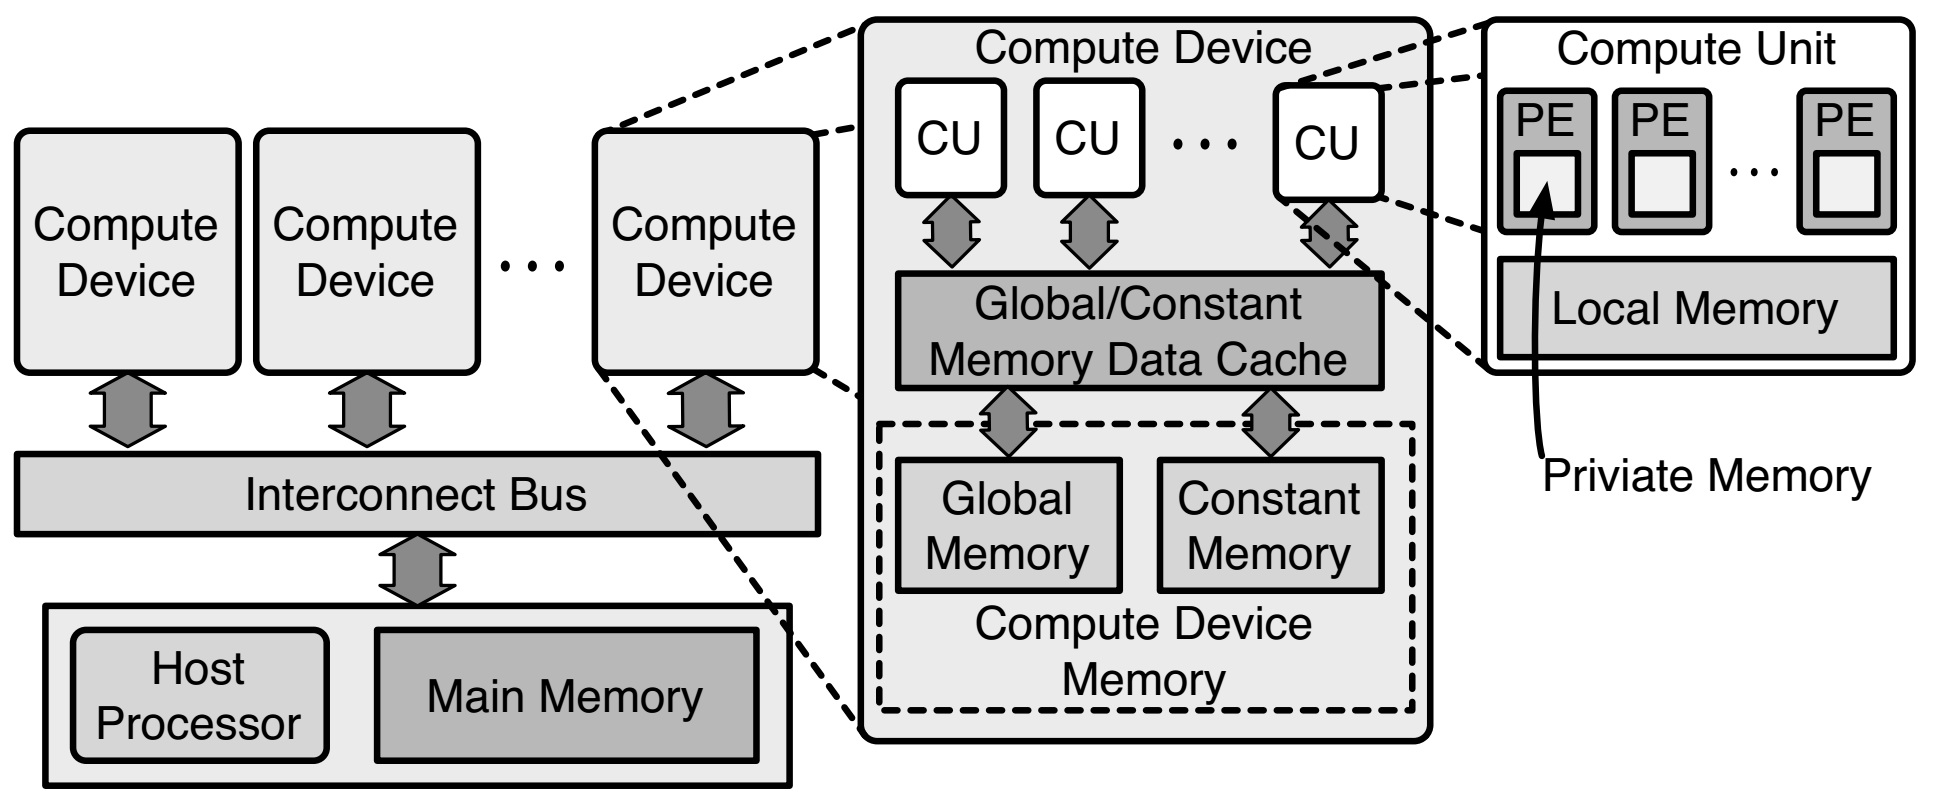
\includegraphics[width=12cm]{ocl_platform_mem_model}
  \caption{OpenCL的平台模型和存储模型\upcite{cell}}
  \label{oclplatformandmem}
\end{figure}

\begin{compactitem}
\item \textbf{平台模型(Platform Model)}
\end{compactitem}

平台模型是OpenCL的抽象低层硬件结构。通过将硬件结构抽象地更为低层,暴露出更多的硬件细节,从而留出更多的编程和优化灵活性;而抽象性又屏蔽了体系结构差异,保证了程序的可移植性。

如图\ref{oclplatformandmem}所示,OpenCL的平台由宿主处理器(Host Processor)和与之互联的一个或者多个计算设备(Compute Device)构成。
每个计算设备又包含一个或者多个计算单元(Compute Unit),而一个计算单元又包含一个或多个处理单元(Processing Element)。
处理单元作为最细粒度的计算承载单位,是一个抽象的标量处理器。

\begin{figure}[htb]
  \centering
  \subfloat[上下文和命令队列\upcite{oclppt}]{%
    \label{comandqueue}
    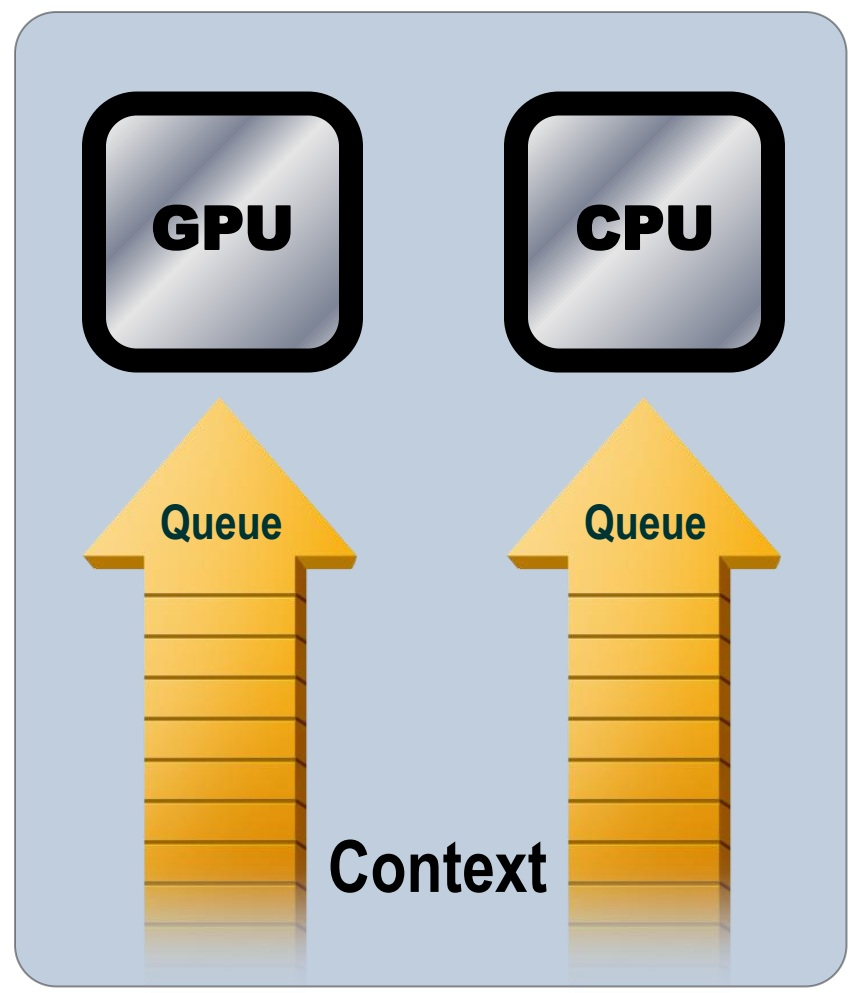
\includegraphics[height=4.5cm]{commandqueue}}\hspace{0.2cm}
  \subfloat[多维索引空间]{
    \label{ndrange}
    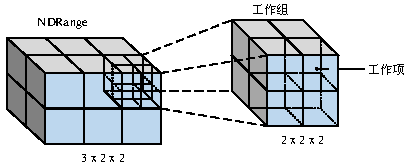
\includegraphics[height=4.2cm]{ndrange}}
  \caption{OpenCL的执行模型}
  \label{oclexecution}
\end{figure}

\begin{compactitem}
\item \textbf{执行模型(Execution Model)}
\end{compactitem}

一个OpenCL程序包括两大部分\pozhehao 宿主程序(Host Program)和Kernel程序(或称内核程序)。

宿主程序用C或者C++编写,运行于宿主处理器之上,通过提交命令(Command)的方式来控制计算设备中的处理单元进行计算,或是控制宿主处理器和计算设备之间的数据传输。
如图\ref{comandqueue}所示,宿主程序会定义一个上下文(Context),上下文中包含了可用的计算设备、待执行的Kernel程序、存储空间等信息。
宿主程序还会为每一个计算设备分配一个或者多个命令队列(Command Queue,或者Queue),并向命令队列中添加命令。随后命令队列就会调度命令进行执行。
命令有三种类型:执行Kernel程序,数据传输,以及同步。

Kernel程序实质上是一个函数,用OpenCL C语言编写,执行于计算设备之上。宿主程序通过提交一个执行Kernel的命令,来启动Kernel程序在计算设备上的执行。
一个Kernel程序有众多的执行实例,对应于一个抽象的多维(一维到三维)索引空间(NDRange Index Space)。
一个Kernel的执行实例对应一个工作项(Work-Item),它是索引空间中的一个最细粒度点,代表着Kernel的一次执行,并根据其在空间中的位置被赋予一个全局索引值(Global ID)。每个工作项都执行相同的Kernel程序,但是由于索引值的不同,各自的执行路径和访问的数据也会不同。
多个相邻工作项组成一个工作组(Work-Group),是对索引空间的更粗粒度分解。根据在索引空间中的位置,工作组也会被赋予一个组索引值(Group ID)。而每个工作组内的工作项,还会根据其组内位置被赋予局部索引值(Local ID)。
OpenCL规定,一个工作组执行于一个计算单元之上,且同一工作组内的工作项是并发执行在计算单元中的处理单元上的。
如图\ref{ndrange}所示,为一个三维的索引空间。该空间包含了$3\times2\times2$个工作组,而每个工作组包含$2\times2\times2$个工作项。

\begin{compactitem}
\item \textbf{存储模型(Memory Model)}
\end{compactitem}

OpenCL的存储模型定义了四个独立的存储空间,分别位于不同的抽象硬件层次之上,且跟执行模型紧密相关。
如图\ref{oclplatformandmem}所示,全局存储(Global Memory)位于计算设备中,任何工作组中的任何工作项都可以读写其中的数据。
常量存储(Constant Memory)是全局存储的一部分,但是其中数据只能被读出而不能被修改。
计算设备还可能提供用以提升全局存储和常量存储性能的高速缓存(Data Cache)。
局部存储(Local Memory)通常位于计算单元之中,仅属于某一个工作组,只能被该工作组中的工作项访问,而对其它工作组来说是不可见的。
私有存储(Private Memory)通常位于处理单元内,是一个工作项所私有的,其它工作项都不可见。

宿主程序可以通过提交数据传输类的命令,来实现宿主处理器的主存(Main Memory)和计算设备的全局存储/常量存储间的数据传输。

\begin{compactitem}
\item \textbf{程序模型(Programming Model)}
\end{compactitem}

这里的程序模型,指的是并行程序的实现方式。OpenCL支持两类并行程序模型,数据并行和任务并行,以及这两类的混合编程。

数据并行是指一个指令序列同时作用于多个存储元素(数据)之上,它是通过定义执行模型中的多维索引空间来实现的。
所有工作项执行相同的Kernel程序,即同一个指令序列;而各个工作项在索引空间中有着不同的索引值,导致根据索引值的访存会访问到不同的数据。
这样一来,同一Kernel程序将同时处理不同数据,实现数据并行。

任务并行是指不同指令序列的同时执行。
实现任务并行,通常是通过在一个或者多个命令队列中,添加多个Kernel执行命令来实现的。


\section{TLD跟踪算法}
\label{sectldalgo}
TLD的命名来自于跟踪(Tracking)-学习(Learning)-检测(Detection)三部分的首字母。
将这三部分有机结合,正是TLD相比于传统跟踪算法的最大区别。
如图\ref{tld}所示,跟踪模块负责计算目标物体在连续两帧间的运动,并提供一个目标候选位置。
它假设目标物体在连续两帧间的运动幅度较小,且目标总是可见的。因此当目标被遮挡或是离开视野时,跟踪模块通常会失效且无法自行恢复。
检测模块将每一帧都看作是独立的,并在整个帧图像中进行搜索检测,从而提供一到多个可能包含目标物体的候选位置。
因此当跟踪模块失效时,检测模块可以重启跟踪。
学习模块会综合考虑跟踪和检测的结果,以最终确定目标物体的位置。
此外,它还会为检测模块提供新的训练数据,以不断提升检测的准确度。

\begin{figure}[htb]
  \centering
  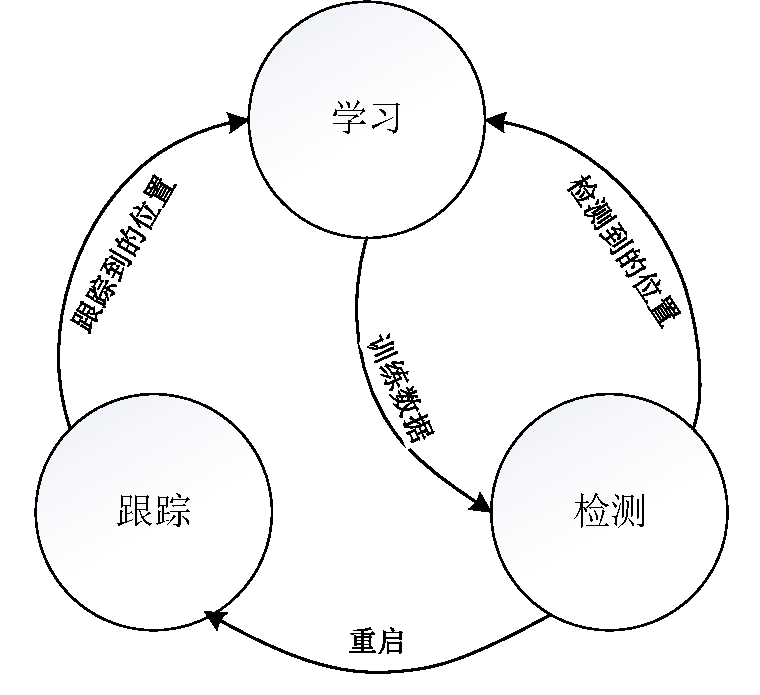
\includegraphics[width=7cm]{tld}
  \caption{TLD跟踪算法的三大部分}
  \label{tld}
\end{figure}

TLD的形式化流程如算法\ref{tldalgo}所示。
更具体地,TLD算法在逐帧运行之前需进行初始化。
初始化的首要任务是构造网格(Grid),即大量的边界框(Bounding Box)。
网格通过用不同的尺度和步长来扫描整幅帧图像得到,与当前帧内容无关,仅与帧大小和目标初始尺度相关。
逐帧运行过程中,检测模块将检测网格中的每一个边界框,找出其中可能包含目标物体的。


\begin{algorithm}[htbp]
  \caption{TLD跟踪算法(对于第$i$帧)}
  \label{tldalgo}
  \algsetup{linenosize=\scriptsize}
  \footnotesize
  \begin{algorithmic}[1]
    \REQUIRE $ $ \\ 当前帧图像$frame[i]$,\\ 前一帧图像$frame[i-1]$,\\ 目标物体在前一帧中的位置(边界框)$lastBB$;
    \ENSURE $ $ \\ 目标物体在当前帧中的位置(边界框)$currentBB$;
    \STATE $trackedBB \leftarrow Tracker( frame[i-1], frame[i], lastBB )$
    \\ $\bullet$ 跟踪模块根据目标物体在前一帧中的位置,计算其在当前帧中的位置,得到$trackedBB$,失效时$trackedBB$为NULL;
    \STATE $detectedBBs \leftarrow Detector( frame[i] )$
    \\ $\bullet$ 检测模块在当前帧中检测出所有可能包含目标物体的边界框,存入$detectedBBs$;
    \STATE $clusteredBBs \leftarrow Cluster( detectedBBs )$
    \\ $\bullet$ 将$detectedBBs$中互相靠近的边界框合并为单个框,存入$clusteredBBs$;
\IF{$trackedBB \neq $ NULL}
    \FOR{\textbf{each} $clusteredBB$ \textbf{in} $clusteredBBs$}
    	\IF{ $Overlap( clusteredBB, trackedBB )  < 0.5$ \AND $NNConf( clusteredBB )  > NNConf( trackedBB )$}
    	\STATE $confidentBBs \leftarrow clusteredBB$ 
    	\ENDIF
    \ENDFOR
    \\ $\bullet$ 从$clusteredBBs$中选出距离$trackedBB$较远,但是置信度更高的边界框,存入$confidentBBs$;
    \IF{ $Sizeof( confidentBBs ) = 1$ }
    \STATE $currentBB \leftarrow confidentBBs[0]$ 
    \\ $\bullet$ 如果$confidentBB$是唯一的,则认为跟踪模块出错,重启跟踪模块;
	\ELSE 
	\STATE $currentBB \leftarrow WeightedAverage( trackedBB, detectedBBs )$ 
	\\ $\bullet$ 否则,以$trackedBB$为主,将$trackedBB$和它附近的$detectedBBs$进行加权平均,得到当前目标位置;
    \ENDIF
    \\ $\bullet$ 跟踪模块有效时,$trackedBB$和$detectedBBs$共同决定$currentBB$;
\ELSE
	\IF{ $Sizeof( clusteredBBs )  = 1$ }
	\STATE $currentBB \leftarrow clusteredBBs[0]$
	\ENDIF
	\\ $\bullet$ 跟踪模块失效时,若存在唯一的$clusteredBB$,则用它来重启跟踪模块;
\ENDIF

	\IF{ $trackedBB \neq $ NULL \AND $Validated( trackedBB ) $ }
    \STATE $ Learn( currentBB, frame[i] )  $
    \ENDIF
    \\ $\bullet$ 若$trackedBB$通过验证,则学习模块根据$currentBB$提取正负样本,训练检测模块。
  \end{algorithmic}
\end{algorithm}

函数$Tracker()$的主要部分是LK(Lucas-Kanade)光流跟踪\upcite{lkoptflow, lkoptflow2},属于跟踪模块。
LK光流跟踪算法会运行两次,第一次用于估计目标物体从$frame[i-1]$到$frame[i]$的运动;第二次逆向运行,根据估计到的$frame[i]$中位置,
计算物体在$frame[i-1]$中的原位置。
通过对比$lastBB$和两次LK光流计算的结果,可以判断出LK光流跟踪是否成功,即跟踪模块是否有效。
%如果LK光流跟踪成功,还需利用最邻近分类计算其结果位置的置信度($NNConf()$)。

%只有置信度高于阈值时,跟踪模块才有效,$Tracker()$才会输出$trackedBB$。

函数$Detector()$主要包括两部分,Fern随机森林\upcite{fern}分类和最邻近分类(Nearest Neighbor Classifier),均属于检测模块。
首先,Fern随机森林将作用于网格中的大量边界框,并得出响应值。该响应值反映了边界框恰好包围目标物体的概率。
随后,响应值高于阈值的边界框将通过最邻近分类,计算出置信度($NNConf()$)。
最邻近分类的模型为一组正负样本图像块,置信度的计算过程为将输入图像块与正负样本逐一进行相似度对比。
这里的相似度使用NCC(Normalized Cross-Correlation,归一化互相关)\upcite{ncc}来度量,
而置信度由输入图像块与正样本的相似程度,以及它与负样本的不相似程度共同决定。
置信度高于阈值的边界框才能作为$Detector()$的输出。
函数$Cluster()$将$Detector()$输出的边界框进行聚类,把互相靠得太近的多个边界框合并为一个,以进一步减少数目。

目标物体在当前帧中的位置最终由学习模块来确定。如果跟踪模块有效,则综合考虑跟踪和检测的结果:
若$clusteredBBs$中存在且仅存在一个置信度高于$trackedBB$的边界框,则认为跟踪模块出错,用检测结果替代跟踪结果;
否则,将跟踪结果与它附近的检测结果进行加权平均,作为最终目标位置。
如果跟踪模块失效,未避免歧义,当且仅当$clusteredBBs$中有唯一边界框时,用来作为最终目标位置。

学习模块还负责决定进行学习的时机,即跟踪结果足够可靠时\pozhehao 跟踪模块有效,且$trackedBB$通过了验证。
$Validated()$函数在两种情况下认为验证通过:$trackedBB$经过最邻近分类得到的置信度足够高;或者在某一历史帧中置信度足够高,
且从那时起跟踪模块从未失效或出错。
学习过程$Learn()$分为两步,提取正负样本和再训练检测模块。
提取正负样本前,需要先计算网格中所有边界框与$currentBB$的重叠率($Overlap()$)。
对于Fern随机森林,选取重叠率低且响应值较高的边界框作为负样本,即``难反例挖掘(Hard Negative Minning)'';
同时选取重叠率高的边界框,并进行随机旋转缩放,作为正样本。
对于最邻近分类器,从$detectedBBs$中选取重叠率低于阈值的边界框作为负样本;
同时以重叠率最高的边界框作为唯一正样本。
再训练Fern随机森林的过程,即是更新每一棵随机树的叶节点权值的过程。通过记录落入每一个叶节点的正负样本总数,更新其权值。
再训练最邻近分类器的过程,即是验证正负样本是否与当前模型冲突(正样本的置信度太低,或负样本置信度太高)的过程。
将冲突的正负样本加入模型中就完成了更新。

通过测试TLD算法的官方串行版本OpenTLD\upcite{opentld},以及借鉴H-TLD\upcite{htld}中的性能分析,
同时考虑到OpenCL会带来的额外开销,本章将以OpenTLD为基础,对其中的计算密集部分和性能瓶颈部分用OpenCL进行高性能实现。
这些部分包括Fern随机森林分类,最邻近分类,学习过程中的重叠率计算、正负样本提取。
LK光流跟踪部分也是计算密集的,但由于OpenTLD所依赖的OpenCV\upcite{opencv}库已提供了OpenCL版本的实现,因此这里不再重复实现。
至于其它部分,有的计算量太小(如确定最终目标位置时,$clusteredBBs$中边界框数量通常很少),有的不适于用OpenCL并行化(如再训练过程中,计算量小且分支过于密集)。

\section{Fern随机森林的高性能实现}
在进行Fern随机森林分类之前,OpenTLD先对网格中的所有边界框进行一次方差过滤,以减少输入随机森林的边界框数量。
边界框对应的图像块的灰度值方差被计算出来,若该方差低于初始帧中目标物图像块的方差,那么该边界框将被过滤掉。
虽然网格中边界框很多,但由于采用了``积分图(Integral Image)''方法,方差过滤十分高效,计算量较小。

如\ref{sectldalgo}节所述,即使加入了过滤步骤,Fern随机森林仍将作用于大量边界框,因此必须十分高效。
TLD算法中,用于分类的特征是基于``像素对比''生成的,即根据边界框提取出图像块,然后在图像块中按照预定模式采样13对像素点,并进行灰度值对比。如果用$0$和$1$来表示对比结果,则13对像素点的对比结果可用一个二进制向量表示,即Fern特征向量。
上述过程被称作特征提取,如图\ref{fernfig}中的``特征提取''部分所示。

\begin{figure}[htb]
  \centering
  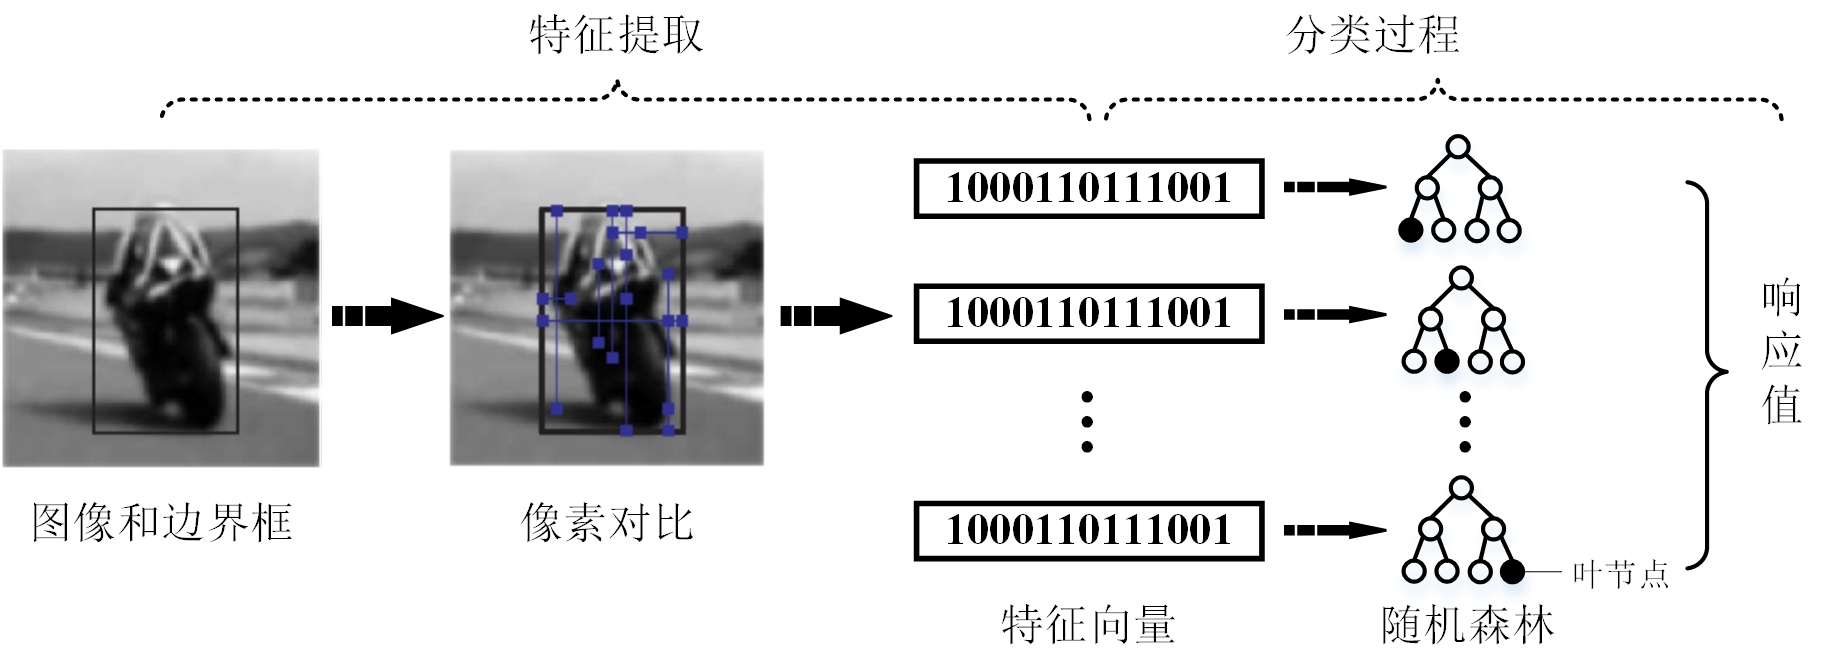
\includegraphics[width=13cm]{fernfig}
  \caption{Fern随机森林分类的流程}
  \label{fernfig}
\end{figure}

由于网格中的边界框有着不同的尺度大小,TLD为每一个尺度定义了10种采样像素点对的模式,每一种采样模式都定义了13个点对的不同采样位置。
因此,每一个边界框通过特征提取后都会得到10个13位的Fern特征向量。
为了对这些特征向量进行分类,TLD针对每一种采样模式(即每一个Fern特征向量)构造一棵随机树,总共10棵随机树构成了Fern随机森林。
随机树的叶节点被赋予权值,代表着边界框包含目标物体的概率。
每个Fern特征向量经过对应随机树的分类后,都会落入该随机树的一个叶节点中。
将10个随机树叶节点的权值进行平均,即得到Fern随机森林的响应值。
上述过程即是Fern随机森林的分类过程,如图\ref{fernfig}中的``分类过程''部分所示。

\subsection{特征提取的并行化}
\label{featureextsec}
特征提取过程的输入为当前帧图像、网格、候选边界框索引、以及像素点对的采样模式;输出为所有候选边界框对应的Fern特征向量。
%在利用OpenCL进行特征提取前,需要对输入数据进行重构。

在本章的高性能实现中,帧图像的灰度值被存储在一个一维数组中。
网格在初始化时就构造好,为一个一维数组,每5个相邻元素代表一个边界框,分别是$\{BBx, BBy, BBw, BBh, scale\_id\}$,即左上角横、纵坐标、宽、高和尺度索引。
因为网格数组在整个跟踪过程中不会变动,因此将它放入OpenCL的常量存储中,供多个Kernel重复使用,而无需每次都进行分配和释放。
候选边界框索引是方差过滤步骤的输出,为一维数组,每个元素($BBid$)都代表着一个候选边界框在网格数组中的位置。
在OpenTLD中,像素点对的采样模式也是一维数组,每4个相邻元素代表一个点对,记为$\{x_1, y_1, x_2, y_2\}$,即两个点在边界框内的坐标。
一种采样模式需要13个点对,而每一种尺度有10种采样模式,考虑所有尺度(最多为21种),采样模式数组中共有$scale\_num
\times10\times13\times4$个元素。
为了更高效的访存,本章将不同采样点的横、纵坐标连续存储,即将$\{x^1_1, y^1_1, x^1_2, y^1_2, ...,x^n_1, y^n_1, x^n_2, y^n_2,\}$
转换为$\{x^1_1, ..., x^n_1, y^1_1, ... , y^n_1, x^1_2, ..., x^n_2, y^1_2, ..., y^n_2\}$。
类似网格数组,采样模式数组也不会变动,因此放入OpenCL的常量存储。

特征提取的计算过程为,从候选边界框索引数组中读出边界框索引,根据该索引在网格数组中读出对应边界框的信息(左上角坐标和尺度索引)。
根据尺度索引访问采样模式数组,得到所需采样的$10\times13$对点在边界框内坐标。
将边界框内坐标和边界框左上角坐标叠加,即得到采样点在图像中的坐标。
最后根据图像中坐标,进行像素点采样对比,构造Fern特征向量。
图\ref{fernext}展示了一次像素点对比,即一个Fern向量中的一位的产生过程。

\begin{figure}[htb]
  \centering
  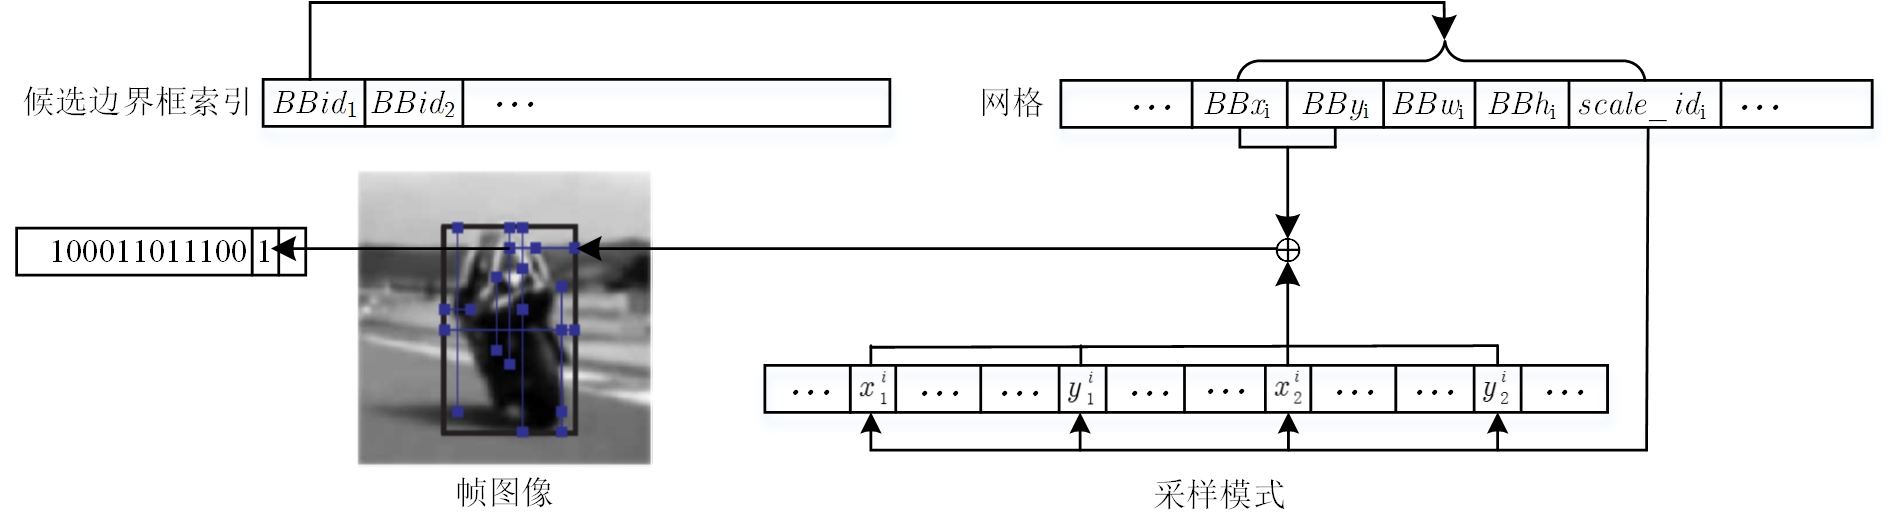
\includegraphics[width=15cm]{fernext}
  \caption{特征提取的流程}
  \label{fernext}
\end{figure}

特征提取的OpenCL并行实现采用一维的索引空间。
一个工作项负责一对采样点的图像中坐标计算、灰度值提取、灰度值对比,即执行一次图\ref{fernext}所示流程。
一个工作组包含130个工作项,负责生成一个边界框的所有(10个)Fern特征向量。
因此一个工作组执行完毕后,每13个相邻工作项需要将各自的像素对比结果整合为一个特征向量。
最后,工作组的数量应当和候选边界框数量相同。
对应的Kernel程序核心代码如表\ref{fernextcode}所示。
第6$\sim$9行中,由于重构了采样模式数组,局部索引值(\texttt{local\_id})连续的工作项将访存连续的存储空间,从而实现了高效的合并访存(Coalesced Memory Access)。
第13行声明了局部存储数组,用于工作项间像素对比结果的高效共享。
最后,由每13个工作项的第一个工作项,负责将对比结果整合为Fern特征向量,写入全局存储中(第18$\sim$22行)。


\begin{table}
\caption{特征提取的Kernel程序}
\label{fernextcode}
\begin{lstlisting}[language=C++, basicstyle=\ttfamily\footnotesize]
__kernel void FernFeatureExtract( __global uchar* img, __constant int* grid, __global int* BB_ids, __constant uchar* sample_patterns, __global int* fern_features,  ... )
{
	...
	BB_id = BB_ids[group_id];
	scale_id = grid[BB_id*5+4];
	x1 = sample_patterns[scale_id*130*4*0+local_id] + grid[BB_id*5]; 
	y1 = sample_patterns[scale_id*130*4*1+local_id] + grid[BB_id*5+1]; 
	x2 = sample_patterns[scale_id*130*4*2+local_id] + grid[BB_id*5]; 
	y2 = sample_patterns[scale_id*130*4*3+local_id] + grid[BB_id*5+1]; 
	pixel1 = img[y1*img_width+x1];
	pixel2 = img[y2*img_width+x2];

	__local int comp_result[130];
	comp_result[local_id] = (pixel1>pixel2) << (12-(local_id%13));
	barrier(CLK_LOCAL_MEM_FENCE);

	...
	if( local_id%13 == 0 )
	{
		fern_feature = comp_result[local_id] | comp_result[local_id+1] | ... | comp_result[local_id+12];
		fern_features[group_id*10+local_id/13] = fern_feature;
	}
}
\end{lstlisting}
\end{table}

\subsection{分类过程的并行化}
\label{fernclassifysec}
获得每一个边界框的10个Fern特征向量后,需要将它们输入随机森林,获得响应值。
从表\ref{fernextcode}的第20行可以看出,保存像素对比结果的特征向量实际上是一个13位二进制整数,
因此高效实现中无需真正建立树结构来逐一判断特征向量的每一元素,
而是采用查找表的方式实现。
13位二进制整数一共有$2^{13}=8192$个可能值,因此可以将随机树实现为8192项的表,每一表项存储一个叶节点的权值。
由于随机森林有10棵树,需分配10个这样的表。
通过将特征向量看做表索引,对对应表进行查表,即可得到对应树的叶节点权值。
对于一个边界框,通过利用它的10个特征向量查找对应的10个表,再将得到的10个权值相加,即可得到响应值。

\begin{table}
\caption{分类过程的Kernel程序}
\label{fernclassifycode}
\begin{lstlisting}[language=C++, basicstyle=\ttfamily\footnotesize]
__kernel void FernClassify( __global int* fern_features, __global float* leaf_weights, __global float* fern_responses, ... )
{
	...
	tree_id = local_id%10;
	BB_id = group_id*20 + local_id/20;

	...
	__local float share_weights[200];	
	fern_feature = fern_features[BB_id*10+tree_id];
	share_weights[local_id] = leaf_weights[tree_id*8192+fern_feature];
	barrier(CLK_LOCAL_MEM_FENCE);

	if( ... && local_id % 10 == 0 )
	{
		fern_response = share_weights[local_id+0] + share_weights[local_id+1] + ... + share_weights[local_id+9];
		fern_responses[BB_id] = fern_response;
	}
}
\end{lstlisting}
\end{table}

分类过程的Kernel程序核心代码见表\ref{fernclassifycode}。程序的主要输入为Fern特征向量数组和叶节点权值数组,输出为每个边界框的响应值。
Fern特征向量数组即是\ref{featureextsec}节的Kernel程序输出,因此该数组可以在全局存储里直接重用。
将随机森林所对应的10个查找表连接在一起,组成了叶节点权值数组,它按顺序存储着$8192\times10$个叶节点权值。
由于每次训练会导致叶节点权值更新,因此该数组需要从主存中拷贝。
当OpenCL程序在GPU上运行时,工作组中的工作项数目太少会导致严重性能下降。
因此,本实现中的一个工作项负责用一个Fern特征向量查表,一个工作组包含200个工作项,即负责20个边界框的响应值计算。
工作项查表的过程就是一个间接访存的过程(表\ref{fernclassifycode},第9、10行)。
通过使用局部存储(\texttt{share\_weights},第8行),间接访存得到的权值可以被工作组高效共享。
因为每10个连续工作项计算同一个边界框的10个叶节点权值,所以它们中的第一个工作项负责将权值累加,计算出响应值(第13$\sim$17行)。

\subsection{与跟踪器重叠执行}
LK光流跟踪和Fern随机森林分类是完全独立的,可以重叠执行。
表\ref{lkferncode}为将光流跟踪和随机森林分类重叠执行的OpenCL宿主程序片段。
由于在每一帧中,经过方差过滤后的边界框数目(\texttt{BB\_num})是不同的,
因此候选边界框索引数组(\texttt{BB\_ids})、Fern特征向量数组(\texttt{fern\_features})、
边界框响应值数组(\texttt{fern\_responses})的长度也会变化,
需要重新创建存储对象,并传输数据(第2、3行)。
帧图像(\texttt{img})和叶节点权值数组(\texttt{leaf\_weights})的内容会变化,但是长度不变,因此可直接从主存传输(写入)到OpenCL全局存储(第6、7行)。
输入数据准备完毕后,将两个Kernel程序(\texttt{FernFeatureExtract}和\texttt{FernClassify})的执行命令加入命令队列(第8、9行),随后再将Kernel的执行结果读出到主存(第10、11行)。
值得注意的是,无论是数据传输还是Kernel执行,上述过程在调用相关OpenCL API时均使用非阻塞版本,即是说将命令写入到命令队列后立即返回,而不是等待命令执行完毕。
写入命令后,命令队列会自动地调度其中的命令在OpenCL计算设备上执行,不再需要干预。
得益于这种机制,在传输数据和执行Kernel程序时,宿主程序无需等待即可调用LK光流跟踪函数进行跟踪(第13行),
从而实现LK光流跟踪和Fern随机森林分类的重叠执行。

LK光流跟踪执行完毕后,还需确认命令队列中的命令是否全部执行完毕(第15行),若未执行完毕,则还需阻塞等待。
最后,释放第2、3行创建的存储对象(第16、17行),以便在处理下一帧时重新创建。

\begin{table}
\caption{LK光流跟踪和Fern随机森林分类的重叠执行}
\label{lkferncode}
\begin{lstlisting}[language=C++, basicstyle=\ttfamily\footnotesize]    
  ...
  TLDCL.CreateMemBufferFernFeatureExtract ( BB_ids, BB_num, fern_features, BB_num*10 );
  TLDCL.CreateMemBufferFernClassify ( fern_responses, BB_num );
  TLDCL.SetKernelArgFernFeatureExtract( );
  TLDCL.SetKernelArgFernClassify( );
  TLDCL.WriteBufferFernFeatureExtract(  img, img.rows*img.cols );
  TLDCL.WriteBufferFernClassify( leaf_weights, 8192*10 );
  TLDCL.EnqueueKernelFernFeatureExtract( );
  TLDCL.EnqueueKernelFernClassify( );
  TLDCL.ReadBufferFernFeatureExtract( fern_features, BB_num*10 );
  TLDCL.ReadBufferFernClassify( fern_responses, BB_num );
    
  LKtrack(img_previous, img_current, lastBB, trackedBB);
    
  TLDCL.SyncCommandQueue(  );
  TLDCL.ReleaseMemObjectFernFeatureExtract( BB_ids, fern_features );
  TLDCL.ReleaseMemObjectFernClassify( fern_responses );
  ...
\end{lstlisting}
\end{table}


\section{最邻近分类器的高性能实现}
在完成Fern随机森林分类后,每个候选边界框的响应值都被计算出来。
只有响应值高于阈值,且排名前100的边界框,才能进入下一步最邻近分类,以计算其包含目标物体的置信度。

\subsection{算法流程}
TLD的最邻近分类算法较为直接。
最邻近分类器维护了两组图像块,即正样本和负样本,它们通常被称作分类器的模型。
分类器首先根据待分类边界框在帧图像中提取对应的图像块,然后将该图像块与模型中的图像块进行一一对比,计算它们的相似度。
在正样本中,输入图像块必然与某图像块最为相似,记它们的相似度为$maxP$。
同理,输入图像块与负样本图像块的最大相似度记为$maxN$。
该边界框的置信度即可按下式算出:
\begin{equation}
\label{nnconfeq}
NNConf = \frac{1-maxN}{2-maxP-maxN} .
\end{equation}
显然,一个边界框的置信度,跟对应图像块与正样本的相似度正相关,跟对应图像块与负样本的相似度反相关。

如\ref{tldalgo}节中所述,这里的相似度是两个图像块的NCC(归一化互相关),其原本定义如下。
对于两幅图像,输入图像$\mathbf{f}$和模板图像$\mathbf{t}$,首先将它们的灰度图保存为二维浮点数组,即每个像素点的灰度用一个$0\sim1$间的浮点数表示。
%然后,将两个二维数组中的所有元素减去各自数组的平均值,即计算归一化灰度。
然后,两幅图像的NCC计算公式为:
\begin{equation}
\label{ncceq}
NCC = \frac{ \sum_{x,y}\mathbf{f}(x, y)\mathbf{t}(x, y) }{ \sqrt{\sum_{x,y}\mathbf{f}(x, y)^2\sum_{x,y}\mathbf{t}(x, y)^2} } ,
\end{equation}
其中$(x, y)$代表像素的横纵坐标。
TLD算法对NCC进行了细微修改。为了避免光照亮度的影响,所有像素的灰度值都会减去所在图像块的平均灰度值。
因此,像素点的灰度不再是归一化的,而可能是正数或者负数。
为了保证NCC的归一化,计算公式修改为:
\begin{equation}
\label{ncceq2}
NCC = \frac{1}{2}( \frac{ \sum_{x,y}\mathbf{f}(x, y)\mathbf{t}(x, y) }{ \sqrt{\sum_{x,y}\mathbf{f}(x, y)^2\sum_{x,y}\mathbf{t}(x, y)^2} } + 1 ).
\end{equation}

\subsection{分类过程的并行化}
一个边界框的最邻近分类过程分为两个步骤\pozhehao 第一步计算对应图像块与每一个样本图像块的NCC,第二步找出$maxP$和$maxN$并计算置信度。
由于有多个边界框需要分类,第一步中需计算的NCC总数目为:边界框数目$\times$样本图像块数目。
考虑到每一次NCC计算需要遍历两个图像块,第一步的计算量将很大,亟需高性能并行化。
而因为边界框数目至多为100个,第二步的计算量会较小,且主要为归约操作(提取最大值),因此不适于用OpenCL进行并行化(归约操作需要大量分支和同步)。
基于上述考虑,本节仅对第一步,即所有NCC的计算,用OpenCL并行化实现。第二步仍然放在宿主程序中处理。

OpenTLD中,最邻近分类器的模型中的图像块大小为$15\times15$,因此根据边界框提取的图像块也会缩放到$15\times15$。
从公式\ref{ncceq2}可以看出,NCC的计算结果与图像块的像素存储方式和像素访问顺序无关。
因此,为了使用OpenCL进行并行化,本节把所有边界框对应图像块的灰度值连续地存储在一个一维数组(\texttt{patches})中。
这样一来,该数组中每$15\times15=225$个连续相邻元素就是一个输入图像块。
同理,本节也把模型中的正负样本图像块连续地存储在一个一维数组(\texttt{p\_n\_samples})中,
且正样本存储在前,负样本存储在后。这样只需记录正、负样本图像块的数目,就能区分某一元素属于正样本还是负样本。
上述两个一维数组即是NCC计算的输入。

\begin{figure}[htb]
  \centering
  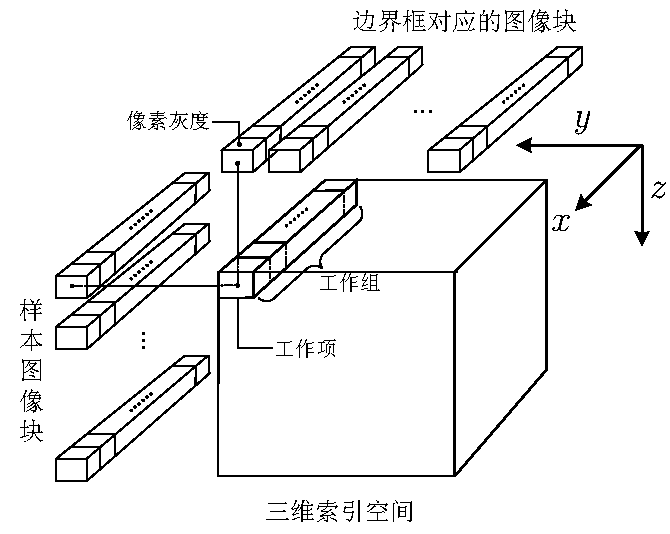
\includegraphics[width=9cm]{nccfig}
  \caption{NCC计算的OpenCL索引空间(注:图中的两组图像块是分别连续存储在两个一维数组中的,这里为了显示清晰将各个图像块分开展示)}
  \label{nccfig}
\end{figure}

NCC计算的OpenCL实现使用三维索引空间,如图\ref{nccfig}所示。
一个工作组负责计算一个边界框对应图像块和一个样本图像块的NCC,因此工作组在$\{x, y, z\}$三个维度上的数目设置为$\{1, $边界框数目$, $样本图像块数目$\}$。
%其中$patch\_num$为边界框数目,$p\_n\_sample\_num$为样本图像块数目。
每个工作项负责一个像素位置,即计算两个图像块中同一位置处的灰度值平方和乘积,因此一个工作组内的工作项数目为$\{225, 1, 1\}$。
故整个三维索引空间的工作项数目是$\{225, $边界框数目$, $样本图像块数目$\}$。
根据公式\ref{ncceq2},将各个像素位置处的计算结果进行累加是不可避免的。
为了实现高效的累加操作,本节将采用树形归约。
由于树形归约要求元素个数为2的次方,因此本节将工作组内工作项数目填充为$\{256, 1, 1\}$,整个索引空间的工作项数目变为$\{256, $边界框数目$, $样本图像块数目$\}$。

\begin{table}
\caption{NCC计算的Kernel程序}
\label{ncccode}
\begin{lstlisting}[language=C++, basicstyle=\ttfamily\footnotesize]    
__kernel void NCC( __global float* patches, __global float* p_n_samples, int p_n_sample_num, __global float* nccs )
{		
    ...
    if ( local_X_id < 225 ) 
    {
        patch_pixel = patches[group_Y_id*225+local_X_id];
        sample_pixel  = p_n_samples[group_Z_id*225+local_X_id];
    }
    else
    {
        patch_pixel = 0;
        sample_pixel  = 0;
    }
    
    __local float patch_squares[256];
    __local float sample_squares[256];
    __local float patch_sample_products[256];
    patch_squares[local_X_id] = patch_pixel * patch_pixel;
    sample_squares[local_X_id] = sample_pixel * sample_pixel;
    patch_sample_products[local_X_id] = patch_pixel * sample_pixel;	
    barrier(CLK_LOCAL_MEM_FENCE);
    
    for( int offset = local_X_size/2; offset > 0; offset >>= 1 ) 
    {
        if ( local_X_id < offset ) 
        {
            patch_squares[local_X_id] = patch_squares[local_X_id+offset] + patch_squares[local_X_id];
            sample_squares[local_X_id] = sample_squares[local_X_id+offset] + sample_squares[local_X_id];
            patch_sample_products[local_X_id] = patch_sample_products[local_X_id+offset] + patch_sample_products[local_X_id];
        }
        barrier(CLK_LOCAL_MEM_FENCE);
    }
	
    if( local_X_id == 0 )
    {	
        square_sum_product = pow( patch_squares[local_X_id]*sample_squares[local_X_id], 0.5 );
        nccs[group_Y_id*p_n_sample_num+group_Z_id] = (patch_sample_products[local_X_id]/square_sum_product + 1) * 0.5;
    }
}
\end{lstlisting}
\end{table}

NCC计算的Kernel程序核心代码见表\ref{ncccode}。
首先,每个工作项根据各自在索引空间中的位置提取像素灰度值(第4$\sim$13行)。
如果是用于填充的工作项,则灰度值置为0,以不影响结果正确性。
由于位置连续的工作项会访问位置连续的全局存储,这里的访存将是高效的合并访存。
第15$\sim$21行计算出公式\ref{ncceq2}中的$\mathbf{f}(x, y)\mathbf{t}(x, y) $、$\mathbf{f}(x, y)^2$以及$\mathbf{t}(x, y)^2$,
并放入局部存储中,以便进行高效累加。
23$\sim$32行进行树形归约,每次循环都将两个工作项的计算结果进行叠加,共需$\log_2256=8$次循环。
最后,每个工作组的第一个工作项负责利用累加结果,计算出NCC,并存入全局存储中(第34$\sim$38行)。
在计算出每个边界框对应的图像块和每个样本图像块之间的NCC后,所有NCC值被传回到宿主程序,由宿主程序负责第二步的置信度($NNConf$)计算。

\section{学习过程的高性能实现}
\label{learnalgosec}
如\ref{sectldalgo}节中所述,当宿主程序整合了检测模块和跟踪模块的结果,确定了当前帧中的目标物体位置($currentBB$),并决定在当前帧进行学习后,
将进入TLD算法的学习过程。
学习过程分为两个步骤。
第一步为提取正负样本,即计算出网格中的所有边界框与$currentBB$的重叠率,然后根据重叠率和Fern随机森林响应值来选取边界框作为正负样本。
第二步为再训练检测模块,即更新Fern随机森林的叶节点权值和最邻近分类器的模型。
第一步中的网格包含了数量巨大的边界框(例如,对于$320\times240$的帧图像将产生60000多个边界框),
逐个计算重叠率并考察响应值将带来巨大的时间开销。
而作为第二步的输入,正、负样本数量通常较少(如训练随机森林的正样本通常为10个,负样本为分类出错的边界框,更为稀少),
故计算量不大,且多为分支操作。
因此,本节仅针对第一步进行基于OpenCL的高性能并行化,而第二步仍然由宿主程序负责。

\subsection{重叠率计算和负样本提取的并行化}
这里的重叠率等价于第\ref{chapbmvc}、\ref{chapijcv}章中所使用的IoU(Intersection over Union),即两个边界框的交集面积除以并集面积。
待提取的负样本为重叠率低于阈值,但Fern随机森林响应值较高的边界框,即分类出错的边界框。
为了提高效率,重叠率的计算和负样本的提取可以在同一个Kernel程序中完成,也就是说在计算出重叠率后,若低于阈值,则检查其响应值,判断是否属于负样本。

显然,重叠率计算和负样本提取的输入为网格、当前目标物体位置($currentBB$)和Fern随机森林响应值;
输出为网格中的所有边界框与$currentBB$的重叠率,以及负样本集合。
与特征提取的Kernel程序(表\ref{fernextcode}和图\ref{fernext})不同,本节中每个工作项负责网格中一个边界框的重叠率计算。
若网格中的边界框仍然按照$\{ ..., BBx_i, BBy_i, BBw_i, BBh_i, scale\_id_i, ... \}$的形式存储在一维数组中,
那么位置连续的工作项在访问同一边界框参数(如$BBx$)时,会访问到间断的存储空间,无法进行合并访存。
由于网格是在初始化时构建的,整个跟踪过程中无需更改,因此在构建原网格数组的同时还可以构造一个以不同方式存储边界框的一维数组,
其内容为$\{BBx_1, ..., BBx_n, BBy_1, ..., BBy_n, BBw_1, ..., BBw_n, BBh_1, ..., BBh_n\}$,称为重构网格数组。
重构网格数组将代替原网格数组作为输入网格,它的构造也只需进行一次,开销可忽略不计。
Fern随机森林的响应值可以重用\ref{fernclassifysec}节的结果数组(\texttt{fern\_responses}),
但是需要插入被方差过滤滤掉的边界框响应值(置为$0.0$)。
由于负样本的数目不确定,且OpenCL中不同工作组内的工作项无法同步,因此采用标记数组来作为输出的负样本集合。
标记数组的长度等于网格中边界框数目,若其中某元素对应的边界框为负样本,则置1,否则置0。

重叠率计算和负样本提取的OpenCL并行实现较为直接,采用一维索引空间。
每一个工作项负责从重构网格数组中提取一个边界框,计算它与$currentBB$的重叠率。
若重叠率低于阈值,则检查响应值数组中对应的响应值,判断是否是负样本。
为了提高OpenCL设备的占用率,将512个工作项组成一个工作组。因此总的工作项数量需要从网格中边界框数量填充为512的倍数。
对应的Kernel程序核心代码如表\ref{overlapcode}所示。
第4$\sim$12行提取了用于重叠率计算的边界框,均可以合并访存。
第15$\sim$23行计算出IoU并存入全局存储中。
最后,25$\sim$30行检查响应值,判断对应边界框是否是负样本。

\begin{table}
\caption{重叠率计算和负样本提取的Kernel程序}
\label{overlapcode}
\begin{lstlisting}[language=C++, basicstyle=\ttfamily\footnotesize]    
__kernel void GetOverlapAndNegativeSample( __constant int* grid_reorg, __global int* currentBB,  __global float* fern_responses, __global float* overlaps, __global uchar* negative_tags )
{		
	...
	int box1x = currentBB[0];
	int box1y = currentBB[1];
	int box1w = currentBB[2];
	int box1h = currentBB[3];
	
	int box2x = grid_reorg[global_id];
	int box2y = grid_reorg[global_id+grid_BB_num];
	int box2w = grid_reorg[global_id+grid_BB_num*2];
	int box2h = grid_reorg[global_id+grid_BB_num*3];
	...
	
	if ( overlap != 0.0 ) {
	    intersec_x =  min(box1x+box1w, box2x+box2w) - max(box1x, box2x);
	    intersec_y =  min(box1y+box1h, box2y+box2h) - max(box1y, box2y);
	    intersec_area = intersec_x * intersec_y;
	    area1 = box1w*box1h;
	    area2 = box2w*box2h;
	    overlap = intersec_area / (area1+area2-intersec_area);
	}
	overlaps[global_id] = overlap;
	
	if ( global_id < grid_BB_num ) {
	  if ( overlap < low_overlap && fern_responses[global_id]>=high_response )
	    negative_tags[global_id] = 1;
	  else
	    negative_tags[global_id] = 0;
	}
}
\end{lstlisting}
\end{table}

\subsection{正样本提取的并行化}
OpenTLD中,学习过程所需的正样本为10个具有最高重叠率的边界框,因此提取正样本的过程就是搜索重叠率前10名的边界框的过程。
虽然该过程是一个典型的归约过程,计算量小且分支较多,但是由于网格中边界框数量巨大,
使用OpenCL并行化仍然可以大幅提高对存储带宽的利用,提升整体性能。

为了搜索重叠率前10的边界框,本节的OpenCL Kernel程序将循环执行10次,每次获取一个边界框在网格数组中的索引位置。
OpenCL索引空间设置为一维,其中的工作项总数与网格中的边界框数目相同。
每个工作项负责读取一个边界框的重叠率,并与工作组中其它工作项进行对比。
1024个工作项组成一个工作组,工作组内将进行树形归约,得到组内具有最大重叠率的边界框索引,并将该索引写入全局存储中。
各个工作组得到的边界框索引将传回宿主程序,由宿主程序再次归约,获得当前具有最大重叠率的边界框。
上述过程等价于将重叠率数组分段,每一段包含1024个边界框的重叠率。
然后在段内和段间进行两步归约,得到最大重叠率。
如图\ref{positivesample}所示,Kernel程序的输入为上一节获得的重叠率数组(\texttt{overlaps}),输出为各个工作组(即各个重叠率数组段)中具有最大重叠率的边界框索引。
宿主程序进行第二次规约后,找出当前具有最大重叠率的边界框并加入正样本中。
显然,若不加修改地再次执行Kernel程序,仍然会得到同一个边界框。
解决该问题的最简单方式就是将重叠率数组中对应的边界框重叠率置为最小值($0.0$)。
为了避免在宿主程序中修改重叠率数组,然后再次传输到OpenCL计算设备,
本节把``当前最大重叠率边界框索引''也作为一个Kernel输入参数。
Kernel程序的第一步就是根据该索引,将重叠率数组对应元素置为0,然后再进行归约。

\begin{figure}[htb]
  \centering
  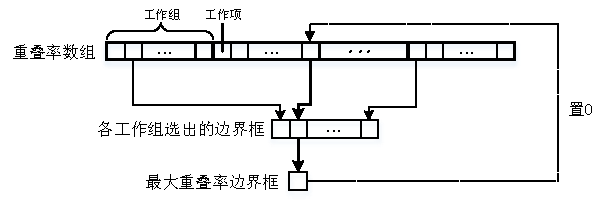
\includegraphics[width=12cm]{positivesample}
  \caption{正样本提取流程}
  \label{positivesample}
\end{figure}

正样本提取的Kernel程序核心代码如表\ref{positivesamplecode}所示。
第4行申请一个局部存储数组\texttt{overlaps\_local},用于保存每次重叠率对比后得到的较高重叠率。
第5行申请的局部存储数组与\texttt{overlaps\_local}对应,用于保存\texttt{overlaps\_local}中每个重叠率对应的边界框索引。
第7$\sim$10行根据输入的``当前最大重叠率边界框索引'',将重叠率数组中的对应元素置为$0.0$。
值得注意的是,第10行的同步语句只作用于各个工作组内的工作项,因此第8行对全局存储数组\texttt{overlaps}的修改可能滞后于某些工作组的归约过程。
但是,被置为$0.0$的\texttt{overlaps}元素只可能被一个工作组用于归约,且负责置$0.0$的工作项正好属于该工作组(由第7行保证),
故这里只需工作组内同步就可以保证各个工作组的归约结果正确。
第12$\sim$14行将重叠率数组段拷贝到局部存储,并将对应的边界框索引填入\texttt{BB\_ids\_local}。
第16$\sim$27行是树形归约过程,每一次循环都将并行对比\texttt{overlaps\_local}中的两个元素,
并记录较高的重叠率和对应的边界框索引。
最后,各个工作组内具有最大重叠率的边界框索引将被写入全局存储中(第29$\sim$31行)。

\begin{table}
\caption{正样本提取的Kernel程序}
\label{positivesamplecode}
\begin{lstlisting}[language=C++, basicstyle=\ttfamily\footnotesize]    
__kernel void GetPositiveSample( __global float* overlaps, int current_top_BB_id, __global int* top_BB_id_in_group )
{			
    ...
    __local float overlaps_local[1024];
    __local int BB_ids_local[1024];

    if ( global_id == current_top_BB_id ) {
        overlaps[current_top_BB_id] = 0.0;
    }
    barrier(CLK_LOCAL_MEM_FENCE);

    overlaps_local[local_id] = overlaps[global_id];
    BB_ids_local[local_id] = global_id;
    barrier(CLK_LOCAL_MEM_FENCE);

    for ( int offset = local_size/2; offset > 0; offset >>= 1) 
    {
        if ( local_id < offset ) 
        {
            if ( overlaps_local[local_id] < overlaps_local[local_id+offset] )
            {
                   BB_ids_local[local_id] = BB_ids_local[local_id+offset];
                   overlaps_local[local_id] = overlaps_local[local_id+offset];
            }
        }
        barrier(CLK_LOCAL_MEM_FENCE);
    }

    if ( local_id == 0 ) {
        top_BB_id_in_group[group_id] = BB_ids_local[0];
    }
}
\end{lstlisting}
\end{table}

全局存储数组\texttt{top\_BB\_id\_in\_group}将被传回宿主程序,由宿主程序进行再次归约,得到当前最大重叠率边界框。
该边界框的索引将作为参数之一,再次调用Kernel程序,直到获取到10个正样本。
如\ref{learnalgosec}节开头所述,完成正、负样本的提取后,检测模块的再次训练不适于用OpenCL并行化,将交由宿主程序负责。
至此,整个TLD算法基于OpenCL的高性能实现已介绍完毕。

\section{实验评测与分析}
本章的实验评测将对比原始OpenTLD版本进行。


\subsection{Kernel性能评测与分析}
在CPU、GPU上,纯Kernel的执行时间;性能移植性问题

算上数据重组、传输等额外开销的执行时间

\subsection{整体性能评测与分析}
全部Kernel在CPU上执行;全部Kernel在GPU上执行(可重叠);各Kernel在适合的设备上执行(最优性能)

\section{小结}
%%*********************第五章******************
\chapter{GPU特定OpenCL Kernel程序的性能移植性提升}
\section{引言}
上一章已经提到,当前从超级计算机到智能手机,异构计算平台已经广泛应用。
而众多异构计算平台中,CPU和GPU仍然是两类最典型的异构计算设备。
近来,英特尔推出的``大量集成核''(Many Integrated Core,MIC)协处理器\upcite{mic}也是一个日渐受欢迎的选择,
例如天河2号超级计算机\upcite{top500th2}就曾借助MIC排名世界第一。
由于共享存储和多指令多数据(MIMD)这两大特点,MIC仍然属于CPU计算设备范畴,可以称作众核CPU。

异构计算平台的发展,让高性能程序设计面临着更多的挑战。
在异构计算平台上编程,最为常见的做法是,为每一个或者每一类计算设备单独编程。
譬如说,对于最常见的CPU-GPU混合计算平台,主流的编程方式为使用CUDA为GPU编程,
同时使用OpenMP为CPU编程。
这样的``设备特定''的编程方式需要编写大量代码,编程产出率(Productivity)较低,
且代码移植性极差,也难以维护。
解决这一问题的最理想方案是设计一种统一的编程模型,
它使得同一代码可以在所有的异构计算设备上运行,且均能达到良好的性能。

在这样的需求下,OpenCL应运而生。如上一章介绍的,OpenCL在设计之初就考虑了跨平台的功能移植性(Functionality Portability),
因而采用了抽象的平台模型来代替具体的硬件体系结构。
使用OpenCL编程的最大便利在于同一代码可以运行在不同的计算设备上,
例如上文中的并行TLD实现,可以在CPU和GPU上无障碍地直接编译运行。
但是,在实验中已经看出,同样的代码在不同设备上有着不同的执行效率,即OpenCL并不能保证性能的移植性(Performance Portability)。
这里的性能移植性,可规范地定义为:
为某个特定体系结构优化的代码,在其它体系结构的计算设备上可达到的性能。

本章主要讨论一类特定的性能移植性,即GPU特定OpenCL Kernel程序在CPU上的性能移植性。
讨论该类移植性的原因有两点。其一,OpenCL的平台模型很大程度上受经典GPU体系结构的启发,
因而编程模型被设计成更适于GPU体系结构的形式。对于那些明显区别于GPU的体系结构,
编译器和运行时会以一些代价较高的方式来模拟GPU体系结构的某些特征。
其二,当前绝大多数OpenCL程序是GPU特定的,或者说是专门面向GPU优化过的。
这些程序通常采用大量的线程,适配GPU式的轮转指令调度方法,以及尽量利用GPU特定的存储层次\upcite{TReporthIllinois, affineloop}。
若将这些程序直接运行在CPU上,通常无法取得好的性能\upcite{OclPP1, OclPP2, OclPP3}。
例如,GPU特定的Kernel通常会同时创建成千上万个线程,以开发工作组间和工作项间(工作组内)的并行性,
但巨大的线程数量对于只有少量重量级核心的CPU设备来说是低效的。
又例如,GPU的存储层次和OpenCL存储模型有着很好的对应,但和CPU的存储结构有很大不同,特别是CPU并没有可编程的局部存储。

为了提升GPU特定OpenCL Kernel程序在CPU上的性能移植性,本章将采用代码转换的方法。
不同于已有的代码转换方法,本章的方法不是对原GPU特定Kernel进行语义上的翻译\upcite{twinpeaks},
也不是单纯地将原Kernel中面向GPU的优化部分向CPU转换适配\upcite{mcuda, efficient},
而是去主动地利用CPU特定的体系结构特征,将原Kernel程序转换为适合多核/众核CPU的形式。
本章的方法基于准确的访存分析,因此生成的代码将去除所有冗余的局部存储数组,
以及它们带来的额外同步开销。
此外,通过从GPU特定的Kernel中提取并行要素和访存局部性信息,本章的方法还可以对循环体进行CPU特定的优化。
本章的目标是一个自动化的源到源(Source-to-Source)代码转换工具链,它以GPU特定的Kernel程序为输入,以一个面向CPU优化过的函数为输出,
其中的优化手段包括数据局部性优化、向量化、去除局部存储、去除冗余同步等。
输出的函数将通过一个调度器在CPU上高效并行运行,而该调度器和本章的代码转换工具将嵌入一个开源的OpenCL运行时中,从而获得一个新的面向CPU体系结构的高性能OpenCL运行时库。
通过用该运行时库替换厂商的原OpenCL运行时(如Intel的\cite{intelocl}),GPU特定的Kernel程序将在CPU上获得较好的性能提升。
因此,在异构计算平台上基于OpenCL实现高性能跟踪器时,可避免为CPU撰写专门的优化代码,而仅需面向GPU进行实现,极大提高编程效率并降低代码维护难度。

本章的贡献主要有以下几点:
\begin{compactitem}
\item 一个全新的工作项折叠方法(\ref{kernelcoalescingsec}节);
\end{compactitem}

该方法基于一种能够准确体现Kernel实际访存模式的线性描述式(\ref{arrayaccessdescriptorsec}节),因此能够去除冗余的局部存储数组和同步。通过消除这些局部存储数组所带来的数据拷贝开销和同步开销,Kernel程序的性能移植性得到很大提升,且更易于后继的CPU特定优化。

\begin{compactitem}
\item 一个适应CPU体系结构的后继优化方法(\ref{postoptimizationsec}节);
\end{compactitem}

该方法作用于工作项折叠后的代码,通过提取原GPU特定Kernel中的并行信息和数据局部性信息,
对代码进行循环级(Loop-Level)的优化。同时,该方法还考虑了多核/众核CPU的体系结构细节,从而在CPU和MIC上获得了较好的性能提升。

\begin{compactitem}
\item 一个CPU特定的OpenCL运行时(\ref{runtimesec}节)。
\end{compactitem}

该运行时整合了本章的代码转换工具和配套的调度器,能够先将GPU特定的Kernel程序进行转换,然后高效地调度在CPU上运行。

此外,\ref{kernelrelatedworksec}节将介绍与本章相关的已有工作,\ref{kernelexperimentsec}节将对本章工作进行实验评测,\ref{kernelconclusionsec}节对本章进行总结。

\section{相关工作}
\label{kernelrelatedworksec}
在本章工作之前,已有很多文献研究如何在多核/众核CPU上提高OpenCL Kernel程序的性能,以提升OpenCL的性能移植性。
这些文献中的方法基本可以分为两类:代码转换方法和自动调优方法。
本章的方法属于第一种类别,即直接将GPU特定的Kernel程序转换为适合在CPU上执行的代码。

代码转换类方法中,最为常用的步骤是工作项折叠\upcite{cell}(Work-Item Coalescing),又称工作项串行化\upcite{mcuda,efficient}(Serialization)。
该步骤可以将一个OpenCL工作组内的所有工作项合并为一个独立、串行的CPU线程,从而得到更粗的线程粒度。
经过此步骤,需要并行执行的线程数量大大降低,在CPU体系结构上执行Kernel程序才变得可行。
现有的代码转换方法在进行工作项折叠和提取SIMD(单指令多数据)并行性时,采用的方案各不相同。
Twin Peaks\upcite{twinpeaks}所使用的方案简单直接,它利用{\tt setjmp}和{\tt longjmp}指令来强行把细粒度的工作项
合并为单个操作系统线程,然后再在工作项内部进行向量化优化,而忽视了工作项间的数据并行性。
分区域串行化(Region Serialization)方法\upcite{mcuda,efficient}通过构造``线程循环(Thread Loop)''来折叠一个工作组内的工作项。
对于工作项间的同步,它采用``循环分裂(Loop Fission)''来实现类似功能,即在同步位置处将线程循环分裂为两个循环。
此外,它还通过自动向量化技术来将线程循环的多次迭代并行化,开发SIMD并行性。
Intel实现的OpenCL运行时\upcite{intelocl}并未开源,仅公开了少量基本方法。
它基于分区域串行化,但是直接生成SIMD指令,因此在开发工作组内的向量并行性方面非常高效\upcite{inteloclguide}。
值得注意的是,上述方法都没有考虑数据局部性,最终生成的代码总是企图尽量多地执行每一个工作项,以减少工作项间的切换。
但这通常会导致间隔、断续的访存模式。解决这一问题的理想方式是将访问同一Cache行的工作项段落交叉执行,提高访存效率。
为此,Stratton等人基于CEAN表达式\upcite{cean},针对数据的空间局部性进行了改进\upcite{TReporthIllinois}。


对于OpenCL的局部存储,当前的代码转换方法通常使用一段全局存储(对于CPU来说即是主存)来进行模拟,
而忽略了CPU中Cache的存在。
至于局部存储带来的同步,Twin Peaks方法直接使用跳转语句来进行模拟,从而导致极大的开销并且破坏了Kernel内的局部性。
上述的其它方法则完全依赖循环分裂,从而导致额外的循环控制开销和变量扩展开销。
目前,CPU体系结构下对局部存储和同步的低效处理已经引起了关注。
在\cite{europar14}中,工作项折叠的同时会分析局部存储数组是否多余,若多余,则将对局部存储数组的访问转换为对全局存储数组的直接访问。
与此类似,Fang等人也提出了自动高效地去除局部存储数组的方法\upcite{groover}。
但是该方法的设计初衷是用于自动调优,因此只是单纯地去除局部存储数组,而没有考虑可能带来的性能影响。
此外,他们还构建了一个分析OpenCL局部存储对性能影响的工具\upcite{aristotle},但是该工具并没有被集成到他们的代码转换器\upcite{groover}中。

第二类方法,即自动调优\upcite{autotuning1, OclPP1}的应用也十分广泛。
该类方法通常首先提取对性能有重要影响的参数,然后通过自动调优程序不断尝试各种参数组合,直到达到最佳性能。
与代码转换类方法相比,自动调优有很多不可避免的劣势。
首先,自动调优需要大量额外编程。除了需要手动编写自动调优程序外,原OpenCL代码还必须重构或者重写,以暴露出影响性能的参数,供调优程序修改。
其次,自动调优方法通常过于耗时且不够鲁棒。在一种体系结构下极大影响性能的参数,在另一体系结构下可能无足轻重,
但自动调优程序自身无法发现问题,从而导致更大的时间开销。
为此,Pennycook等人提出了一种体系结构无关的方法\upcite{OclPP1},以发掘出在不同体系结构下均能获得可接受的(而不是最优的)性能
的参数组合。

以在异构平台上获得最大的性能移植性为目标,Phothilimthana等人的工作综合了上述两类方法\upcite{asplos}。
他们引入并扩展了PetaBricks语言\upcite{petabricks}和相应的编译器,从而能够自动地为多种设备生成OpenCL代码。
后继的OpenCL代码优化过程则主要是基于自动调优的。

\section{数组访问的线性描述式}
\label{arrayaccessdescriptorsec}
准确地识别OpenCL Kernel程序对局部存储和全局存储的访存模式是进行高性能代码转换的关键。
访存模式通常通过使用编译器前端分析Kernel程序,然后构造数组访问描述来获取。
但是,绝大部分已有的数组访问描述都是面向嵌套循环的,主要用于自动并行化、私有化等循环级优化。
而且,这些描述中通常还引入了一定程度的估计,导致精度不足,无法用于分析OpenCL工作项间的依赖性。
典型的例子有Shen等人的三元组标记\upcite{shen},Paek等人的线性访存描述子\upcite{paek}等。
这些描述仅记录了循环体中数组访问的一些基本特征,比如循环变量、循环变量上下界、访存跨度等。
由线性等式和线性不等式构成的线性约束系统(Linear Constraint System)也被用于描述数组访问,
例如Trilolet等人提出的域描述\upcite{triolet},Balasundaram等人的数据访问描述子\upcite{bala},
以及新近提出的多面体模型\upcite{pmodel}等。但它们仍然不是面向并行程序的。
与本节的线性描述式最为接近的是Jang等人的工作\upcite{itpds11},他们以访存矩阵加偏移向量的形式描述嵌套循环,
并用来指导从循环嵌套到数据并行程序的转换。
Fang等人将这一工作应用在了OpenCL Kernel上\upcite{aristotle},构造出了一个自动分析工具。
通过将访存矩阵、偏移向量和体系结构参数输入工具,就能分析出局部存储对性能的影响。

本节将提出一个新的数组访问线性描述式。相比上述的描述方法,它更加的精确,但又足够灵活。
该描述基于一个重要假设,即绝大多数GPU特定Kernel程序中,数组访问模式都是线性的。
这一假设是通过分析大量GPU特定Kernel程序得出的,
譬如,在Nvidia GPU Computing SDK\upcite{nvidiasdk}和SHOC\upcite{shoc}测试集中,只有包含了间接访存(一个数组的访问索引是另一数组的元素)的Kernel才可能违反该假设。
换句话说,即使本节的线性描述式局限于线性或者直接的存储访问,它仍然可以覆盖绝大多数的GPU特定Kernel程序。

本节的数组访问线性描述式由下标函数和访问约束共同组成。
对于OpenCL Kernel程序中的每一个数组访问,都使用一个线性下标函数和一组线性访问约束来进行描述。
下标函数的函数值是对应数组的访问索引,表示的是该次访存可能访问到的数组元素位置;
每一条访问约束都是一个线性等式或者不等式,根据循环边界和条件语句产生,用以约束数组访问索引的范围。
下标函数和访问约束中的变量包括:
工作组的组索引值(Group ID)、工作项的局部索引值(Local ID)、包围该次访存的各层循环的循环变量、以及Kernel程序的输入参数。
如果这些变量的某一赋值满足了所有访问约束,则Kernel一定会访问对应数组的下标函数值处的元素。

\begin{table}[htb]
	\centering
	\caption{原始的GPU特定矩阵乘法Kernel程序}
	\fbox{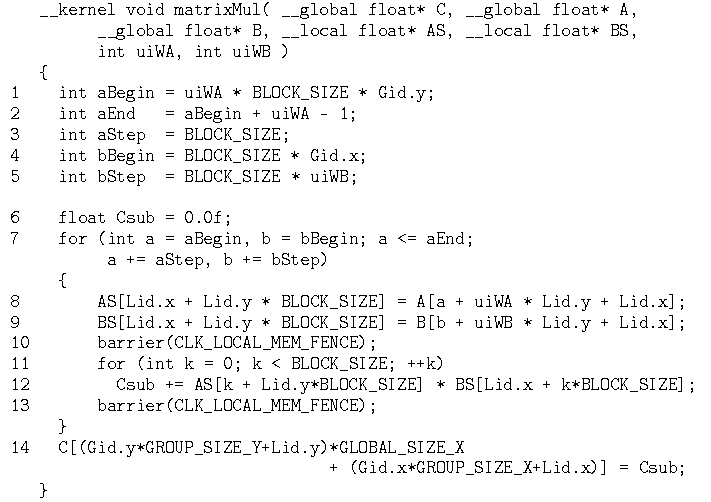
\includegraphics[width=12cm]{fig1-3.pdf}}
	\label{orgkernel}
\end{table}

下面以实例来说明本节所采用的数组访问描述式。
表\ref{orgkernel}为来自Nvidia GPU Computing SDK的矩阵乘法OpenCL Kernel程序,它面向GPU实现了$\bm{C}=\bm{A}\times \bm{B}$。
为了清晰易懂,原Kernel中的一些变量名被修改,此外,{\tt Lid} 代表工作项的局部索引值,{\tt Gid}代表工作组的组索引值。
在Kernel的外层循环中(第7$\sim$13行),一共有6处数组访问:
第8行的写$\bm{AS}$和读$\bm{A}$,
第9行的写$\bm{BS}$和读$\bm{B}$,
第12行的读$\bm{AS}$和读$\bm{BS}$。
作为示例,对于$\bm{AS}$和$\bm{A}$的3处数组访问的线性描述式如图\ref{desriptor1}所示。
其中,$f$代表线性下标函数,$Constraint$代表线性访问约束的集合,
$Iter_x$($x = a, b, k$)代表循环正规化(Loop Normalization)后的循环变量。
对于数组访问$\texttt{A[a + uiWA * Lid.y + Lid.x]}$,得到的线性下标函数是$f^{read}_{A}$,其值覆盖了Kernel执行时对数组$\bm{A}$的所有可能的访问位置。
线性约束集合$Constraints^{read}_{A}$通过约束$f^{read}_{A}$中变量的取值,限制了上述访问位置的范围。
由于对数组$\bm{BS}$和$\bm{B}$ 的访问描述式与图\ref{desriptor1}非常类似,因此不再单独列出。

\begin{figure}[htb]
	\scalebox{0.8}{$\left\{ \begin{array}{l}
		f_{\bm{A}}^{read} = (uiWA \times BLOCK\_SIZE \times Gid.y + BLOCK\_SIZE \times Ite{r_a}) + uiWA \times Lid.y + Lid.x\\
		Constraint_{\bm{A}}^{read} = \{ Ite{r_a} \ge 0\;;\;\;Ite{r_a} < uiWA/BLOCK\_SIZE;\;Gid.y \ge 0;\;\\
		\;\;\;\;\;\;\;\;\;\;\;\;\;\;\;\;\;\;\;\;\;\;\;\;\ \ \ \ \ \ Gid.y < GLOBAL\_SIZE; \ 
		Lid.x \ge 0;\;Lid.x < BLOCK\_SIZE;\;Lid.y \ge 0;\\
		\;\;\;\;\;\;\;\;\;\;\;\;\;\;\;\;\;\;\;\;\;\;\;\;\ \ \ \ \ \ Lid.y < BLOCK\_SIZE\} 
		\end{array} \right.$}
	\vspace{0.1in}
	
	\scalebox{0.8}{$\left\{ \begin{array}{l}
		f_{\bm{AS}}^{write} = Lid.x + Lid.y \times BLOCK\_SIZE\\
		Constraint_{\bm{AS}}^{write} = \{ Lid.x \ge 0;\;Lid.x < BLOCK\_SIZE;\;Lid.y \ge 0;\;Lid.y < BLOCK\_SIZE\} 
		\end{array} \right.$}
	\vspace{0.1in}
	
	%\hspace{1.025in}\scalebox{0.8}{$\left\{ \begin{array}{l}
	%f_B^{read} = (BLOCK\_SIZE \times Gid.x + BLOCK\_SIZE \times uiWB \times Ite{r_b}) + uiWB \times Lid.y + Lid.x\\
	%Constraint_A^{read} = \{ Ite{r_b} \ge 0;\;\;Ite{r_b} < uiWB/BLOCK\_SIZE;\;Gid.x \ge 0;\;Gid.x < GLOBAL\_SIZE;\\
	%\;\;\;\;\;\;\;\;\;\;\;\;\;\;\;\;\;\;\;\;\;\;\;\;\ \ \ \ \ \ \ Lid.x \ge 0;\;Lid.x < BLOCK\_SIZE;\;Lid.y \ge 0;\;Lid.y < BLOCK\_SIZE\} 
	%\end{array} \right.$}
	%
	%\hspace{1.03in}\scalebox{0.8}{$\left\{ \begin{array}{l}
	%f_{BS}^{write} = Lid.x + Lid.y \times BLOCK\_SIZE\\
	%Constraint_{BS}^{write} = \{ Lid.x \ge 0;\;Lid.x < BLOCK\_SIZE;\;Lid.y \ge 0;\;Lid.y < BLOCK\_SIZE\} 
	%\end{array} \right.$}
	%\vspace{0.05in}
	
	\scalebox{0.8}{$\left\{ \begin{array}{l}
		f_{\bm{AS}}^{read} = Ite{r_k} + Lid.y \times BLOCK\_SIZE\\
		Constraint_{\bm{AS}}^{read} = \{ Ite{r_k} \ge 0;\;\;Ite{r_k} < BLOCK\_SIZE;\;Lid.y \ge 0;\;Lid.y < BLOCK\_SIZE\} 
		\end{array} \right.$}
	
	%\hspace{1.03in}\scalebox{0.8}{$\left\{ \begin{array}{l}
	%f_{BS}^{read} = Lid.x + Ite{r_k} \times BLOCK\_SIZE\\
	%Constraint_{BS}^{read} = \{ Ite{r_k} \ge 0;\;\;Ite{r_k} < BLOCK\_SIZE;\;Lid.x \ge 0;\;Lid.x < BLOCK\_SIZE\} 
	%\end{array} \right.$}
	\caption{矩阵乘法Kernel中读$\bm{A}$、写$\bm{AS}$和读$\bm{AS}$的数组访问线性描述式}
	\label{desriptor1}
\end{figure}

有了本节中提出的数组访问线性描述式的帮助,
对GPU特定OpenCL Kernel程序的代码转换将分为两步进行:
基于分析的工作项折叠和适应体系结构的后继优化。
这两步的目的都是提升Kernel程序在多核/众核CPU上的性能。

\section{基于分析的工作项折叠}
\label{kernelcoalescingsec}
工作项折叠(或者串行化)的目的是加粗线程粒度,通常会将一个工作组内的所有工作项合并为一个独立的CPU线程。
标准的折叠方法是构建线程循环嵌套。
该循环嵌套的层数和Kernel的索引空间维度一致,
各层的循环变量与工作项的局部索引对应,最内层的循环体就是原Kernel程序,如图\ref{serialize}(a)、(b)所示。

但是构建这样的线程循环并非易事,面临的最大挑战就是Kernel程序中同步语句(如\texttt{barrier()})的存在。
当前最先进的工作项折叠方法均采用循环分裂来解决同步问题。
图\ref{serialize}(c)、(d)展示了构建线程循环并使用循环分裂的例子。
图\ref{serialize}(d)中,由于\texttt{barrier()}语句的存在,线程循环在同步语句处被分裂为两个线程循环。
循环分裂所带来的额外开销主要有两部分,一是额外的循环控制语句,
二是可能导致的变量扩展(Variable Expansion)。
变量扩展指的是,当分裂出的两个循环的循环体中有共用变量时,由于执行路径的改变,需要保存第一个循环每次迭代后的共用变量值。
否则,第二个循环得到的将只有前一循环最后一次迭代得到的共用变量值。
如果工作组内的工作项数目较多,变量扩展将导致大量的额外访存开销(变量将无法放入寄存器中)。
为此,本节将基于数组访问描述式进行准确的工作项间依赖性分析,将不必要的同步语句预先消除,
从而从根本上避免循环分裂。具体细节将在\ref{dependenceanalysissec}节中介绍。

\begin{figure}[htb]
\centering
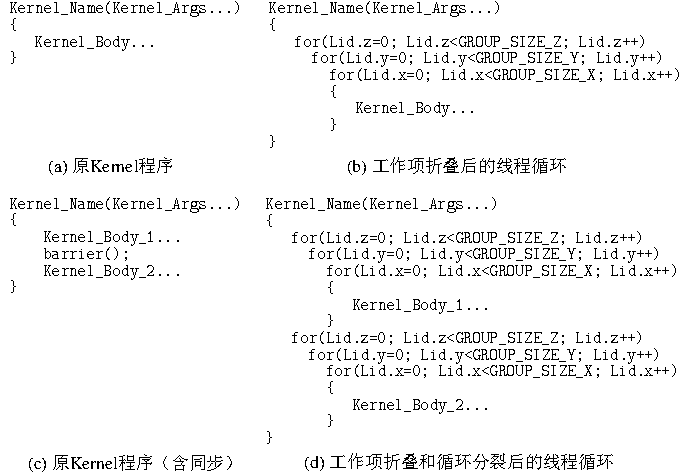
\includegraphics[width=13.25cm]{fig3.pdf}
\caption{通过构建线程循环来进行工作项折叠}
\label{serialize}
\end{figure}

工作项折叠过程中,另一极大影响性能的要素就是OpenCL局部存储的使用。
使用在局部存储中分配的数组是GPU特定Kernel程序非常常用的性能优化方法。
因为OpenCL局部存储直接对应着GPU的高速片上存储,访问局部存储数组会十分高效。
但是,CPU体系结构中并没有能够与局部存储对应的硬件支持,因此现有的OpenCL运行时只能用一段主存空间来模拟局部存储的功能。
在这种情况下,如果不加区分地使用局部存储数组,很可能由于额外的数据拷贝和附带的同步,导致性能反而下降。
目前已有的工作项折叠方法均没有对局部存储数组进行有效的处理,
而本节的一大创新就是在折叠过程中去除冗余的局部存储数组,从而提升Kernel程序性能。
对局部存储数组是否冗余的相关分析,以及对应的去除过程,都是基于数组访问描述式的,
具体将在\ref{localmemeliminatesec}节中进行介绍。

\subsection{去除冗余的局部存储数组}
\label{localmemeliminatesec}
局部存储数组在GPU特定的OpenCL Kernel程序中的作用可以分为以下4种类型:
\begin{compactitem}
\item[1)]{\textbf{数据缓存}:为了提升Kernel程序的时间和空间局部性,将经常访问或者将被重复访问的数据缓存在局部存储中,从而使延迟较长的全局存储访问变为更快速的局部存储访问。}
\item[2)]{\textbf{数据重组}:通过合并访存的方式从全局存储中读出数据,然后以另一种形式存入局部存储中,以避免后续对局部存储的访问发生组冲突(Bank Conflict)。一个典型的例子就是矩阵转置相乘($\bm{C} = \bm{A}\times \bm{A}^{\rm T}$)Kernel\upcite{oclbestpractice}中,$\bm{A}$按行从全局存储中读出,之后按列存入局部存储数组。}
\item[3)]{\textbf{数据交换}:将工作项执行的中间结果存入局部存储中,然后由其它工作项读出。这种作用类型不仅能够在工作项间交换数据,还能避免多个工作项进行重复的计算。}
\item[4)]{\textbf{防止寄存器溢出}:如果Kernel内申请的私有变量过多,导致执行所有工作项所需的寄存器不足,那么这些私有变量就会溢出到低速的片外存储(显存)内,导致性能大幅下降。这种作用类型将局部存储看作是私有存储的扩展,用于存储更多的工作项私有数据。 }
\end{compactitem}

在CPU体系结构下,第3)种作用类型的OpenCL局部存储数组也是必需的,
因此在工作项折叠过程中不可去除。
具有第4)种作用的局部存储数组也不可去除,因为该局部存储数组是用于存放中间结果的,一旦去除将无处存放溢出的数据。
对于第2)种作用类型的局部存储数组,尽管CPU只是用一段主存空间进行模拟,并且会导致一次额外的数据拷贝,本节也仍然将其保留。
原因在于其中的数据进行过重组,后续的访存将变得高效,从而很可能提升最终性能。
至于第1)种作用类型,局部存储数组就完全多余了。
因为CPU体系结构中的多级Cache具有完全相同的功能,所以使用局部存储数组是毫无意义的,还会导致额外的数据拷贝。
要准确去除第1)种作用类型的数组,需要首先通过分析判别局部存储数组的作用类型,然后将对原数组的访问转换为对全局存储数组的访问。

如果一个局部存储数组不具备第3)和第4)种作用,但是具备第1)或者第2)种(又或者两种皆有之),
那么Kernel程序对它的一系列访问必然满足下列过程\upcite{oclprogrammingguide}:
\begin{compactitem}
\item[$\rightarrow$]{从全局存储数组中读出数据,再存入该局部存储数组中。} 
\item[$\rightarrow$]{可能在工作组内进行一次同步,以确保之后每个工作项都可以安全地读取到其它工作项写入的数据。} 
\item[$\rightarrow$]{从该局部存储数组中读出数据,并使用数据进行计算。} 
\item[$\rightarrow$]{如果访存过程是循环的,则还需要一次同步,以避免有的工作项还未利用该局部存储数组中的数据进行计算。}
\end{compactitem}
例如表\ref{orgkernel}中,$\bm{AS}$和$\bm{BS}$这两个局部存储数组就是仅用于缓存数据的。
对这两个数组的访问完全符合上述过程。
如表\ref{orgkernel}的第8、9行所示,数组$\bm{AS}$和$\bm{BS}$中的数据直接来自于全局存储数组$\bm{A}$和$\bm{B}$。
而第10、13行即是所需的两次同步。

只有当同时满足下列两个条件时,局部存储数组的读访问才能被转换为直接的全局存储数组读访问:
\begin{compactitem}
\item[(1)]{存在一个与该局部存储数组读访问相对应的局部存储数组写访问:如果将写访问的描述式中的某些变量替换为读访问中的变量,二者的数组访问描述式(包括下标函数和访问约束)可变得完全相同。}
\item[(2)]{(1)中的局部存储数组写访问的数据是来自于全局存储数组的。该条件可以通过检查``定义—使用链(Define-Use Chain)\upcite{compilerbook2}''来验证,且通常情况下,局部存储数组写访问和对应的全局存储读访问是相邻的。}
\end{compactitem}
如果一个局部存储数组具有作用类型3)或者4),那么对它的读访问将无法满足上述两个条件,因为数组中的元素均来自于中间计算结果,而不是来自全局存储。

将局部存储数组的读访问转换为全局存储数组读访问的过程,
就是找出所有满足上述两个条件的局部存储数组读操作,然后将它们用条件(2)中的全局存储数组读操作替换。
随后,与条件(1)中的局部存储数组写访问相关的语句将变为``死代码(Dead Code)'',被编译器自动地去除。
一个典型的例子就是图\ref{desriptor1}中的那对局部存储数组读写:
%\begin{small}
\begin{equation}
\small
\left\{ \begin{array}{l}
f_{\bm{AS}}^{write}=Lid.x + Lid.y \times BLOCK\_SIZE\\
Constraint_{\bm{AS}}^{write}=\\ \{ Lid.x \ge 0;\;Lid.x < BLOCK\_SIZE;\ Lid.y \ge 0;
\\ \;Lid.y < BLOCK\_SIZE\} 
\end{array} \right.,
\label{eq4.1}
\end{equation}
\begin{equation}
\small
\left\{ \begin{array}{l}
f_{\bm{AS}}^{read} = Ite{r_k} + Lid.y \times BLOCK\_SIZE\\
Constraint_{\bm{AS}}^{read} = \\
\{ Ite{r_k} \ge 0;\;\;Ite{r_k} < BLOCK\_SIZE;\ Lid.y \ge 0;\\ \;Lid.y < BLOCK\_SIZE\} 
\end{array} \right..
\label{eq4.2}
\end{equation}
%\end{small}
如果将公式(\ref{eq4.1})中的$Lid.x$ 用公式(\ref{eq4.2})中的$Iter_k$ 替换,那么上面两个数组访问描述式将变得一样,即满足了条件(1)。
此外,根据表\ref{orgkernel}第8行,公式(\ref{eq4.1})的数据来源是全局存储数组$\bm{A}$ :
\begin{equation}
\small
\begin{array}{l}
f_{\bm{A}}^{read} = (uiWA \times BLOCK\_SIZE \times Gid.y + \\ BLOCK\_SIZE \times Ite{r_a})
 + uiWA \times Lid.y + Lid.x,
\end{array}
\label{eq4.3}
\end{equation}
因此条件(2)也满足了。
综上,将公式(\ref{eq4.2})对应的局部存储数组读访问转换为直接的全局存储数组读访问是可行的。
通过将公式(\ref{eq4.3})中的$Lid.x$替换为$Iter_k$,然后用变量替换后对应的读操作代替公式(\ref{eq4.2})对应的读操作,即可完成转换:
\begin{equation}
\begin{array}{l}
\small
f_{\bm{AS}}^{read} = Ite{r_k} + Lid.y \times BLOCK\_SIZE\\
 \Rightarrow \\
f_{\bm{A}}^{read} = (uiWA \times BLOCK\_SIZE \times Gid.y +\\ BLOCK\_SIZE \times Ite{r_a})
 + uiWA \times Lid.y + Ite{r_k}
\end{array}.
\end{equation}

上述的转换条件和方法只考虑了可行性,即可用于所有没有数据交换功能和防止寄存器溢出功能的局部存储数组。
但是,对于具有数据重组功能的局部存储数组,上述方法虽然可行但不会带来性能提升。
因此这里再附加一个启发式的条件,以确保局部存储数组不具有数据重组的作用:
\begin{compactitem}
\item[(3)]{考察条件(1)中的局部存储数组写访问,以及(2)中的全局存储数组读访问,它们的下标函数中变量$Lid.x$必须具有相同的系数(或者都不含变量$Lid.x$,即系数为$0$)。}
\end{compactitem}
例如,在公式(\ref{eq4.1})和(\ref{eq4.3})中,下标函数$f^{write}_{\bm{AS}}$和$f^{read}_{\bm{A}}$的$Lid.x$ 变量系数均为$1$,
并且公式(\ref{eq4.1})和公式(\ref{eq4.2})覆盖了Kernel对局部存储数组 $\bm{AS}$的所有访问。
因此基于条件(3),可以确定局部存储数组$\bm{AS}$不具有数据重组的作用,
去除它将在CPU体系结构下带来性能提升。

通过去除所有仅具有数据缓存作用的局部存储数组,并且将对于这些数组的访问转换为对全局存储数组的直接访问,
工作项折叠后的Kernel性能将获得明显提升。
表\ref{localmemremoved}(代码的行号与表\ref{orgkernel}一致)展示了去除冗余的局部存储数组后的矩阵乘法代码。
其中,局部存储数组$\bm{AS}$和$\bm{BS}$由于仅作为数据缓存使用,都被去除掉了。

\begin{table}[htb]
\centering
\caption{去除冗余的局部存储数组后的矩阵乘法Kernel代码片段}
\fbox{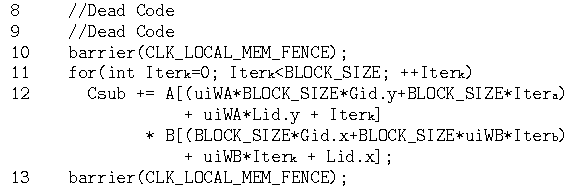
\includegraphics[width=10cm]{fig4.pdf}}
\label{localmemremoved}
\end{table}

\subsection{依赖性分析和同步语句消除}
\label{dependenceanalysissec}
如果一个工作组中的不同工作项会访问相同的存储位置,那么同步通常是必要的,否则Kernel程序的执行结果将是不确定的。
在Kernel程序中,作为同步点的\texttt{barrier}语句经常会离局部存储数组的访问非常近,这是因为局部存储是由工作组内的所有工作项所共享的存储空间。
但是,\texttt{barrier}语句的存在并不代表工作项间确实存在依赖性(写后读相关、读后写相关、或写后写相关),而由于依赖所产生的同步才是真正不可消除的。
例如,\ref{localmemeliminatesec}节所述的4种局部存储数组作用类型中,只有数据交换才会导致真正的数据依赖,
即一个工作项在获取到另一工作项的中间结果前,无法继续执行。
具有其它3种作用类型的局部存储数组也可能引入同步语句,但是工作项间并没有真正的依赖性。
如果各个工作项直接从全局存储中获取所需的数据,同步语句则不再必要。
也即是说,如果\texttt{barrier}语句是由仅具有数据缓存或数据重组功能的局部存储数组引入的,那么它是可以随着局部存储数组一起去除掉的。

在CPU体系结构下,同步语句的作用可能存在两面性。
工作项折叠时,如果在同步语句位置进行循环分裂,则一定会导致额外的开销,如循环控制和变量扩展。
但是循环分裂的同时也改变了工作组的执行流程,从而也可能带来更好的时间和空间局部性。
对于这个两面性问题,本节的解决方案是:
在工作项折叠过程中忽略同步语句可能带来的好处,尽可能地去除同步语句。
然后在线程循环的后继优化中针对具体的体系结构细节,重新开发数据局部性,具体将在\ref{localityreexploresec}节中介绍。

在去除了冗余的局部存储数组之后,就可以开始进行同步语句的消除。
但是,单纯地删除所有的\texttt{barrier}语句是不安全的,因为同步语句可能还服务于其它未被去除的局部存储数组,也可能是由于全局存储数组而导致的同步。
为了检查一个同步语句是否可以被安全地删除,需要进行依赖性分析。
这里的依赖性分析和经典的依赖性分析有很大的不同,因为它是在不同的工作项间进行的。
而在工作项内代码是串行执行的,因此无需考虑工作项内的依赖性,该依赖性也与同步无关。
本节依赖性分析的核心思想是:如果两个工作项访问了同一局部存储数组或全局存储数组(其中至少有一个访问是写访问),
并且访问的数组区域有重叠,那么这两个工作项间就存在依赖性。

依赖性分析是针对每一条\texttt{barrier}语句逐次进行的。
首先将同步语句也看作是基本块(Basic Block)边界,将Kernel代码划分为多个基本块。
虽然引入了同步,但是这里基本块的概念和经典编译理论中的概念是一致的,
即基本块是一个包含了尽量多的语句的代码段,其中任意一条语句的执行,意味着块内的其它语句也一定会执行。
然后需要考察每一对满足下列条件的数组访问:
两个数组访问分别来自位于同步语句前、后的基本块;两个数组访问针对同一个局部存储数组或全局存储数组;
其中一个数组访问是写访问。
如图\ref{dependence}的上半部分所示,虚线矩形框代表的是不同控制语句导致的基本块划分,箭头指向的是需要考察其中数组访问的两个基本块。
图\ref{dependence}的下半部分强调了对数组访问的考察是针对不同工作项的。
考察一对数组访问时,需要将二者对应的数组访问描述式进行联立,构成一个丢番图不等式系统(Diophantine Inequation System)。
如果该不等式系统有解,且解中不要求所有的工作项局部索引值相等,那么真正的依赖存在,对应的\texttt{barrier}语句不可删除。

\begin{figure}
	\centering
	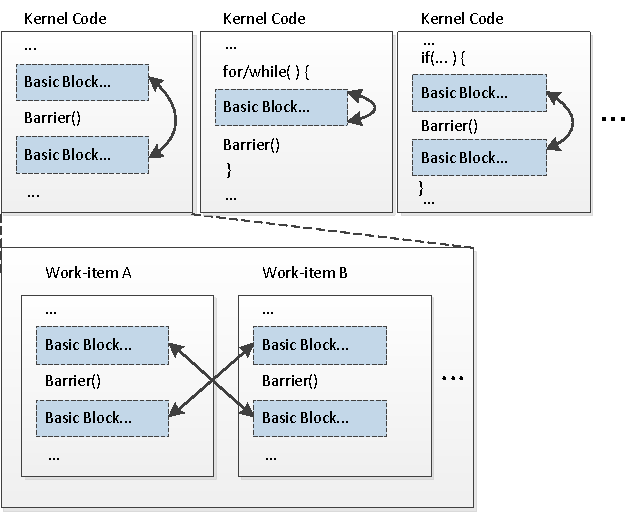
\includegraphics[width=10.5cm]{fig5.pdf}
	\caption{依赖性分析示意图}
	\label{dependence}
\end{figure}

公式(\ref{eq4.5})展示了上述不等式系统的构建过程:
\begin{equation}
\small
\begin{array}{l}
\left\{ \begin{array}{l}
{f_1} = \overrightarrow {\bm{Co{e_1}}}  \cdot {\overrightarrow {\bm{Var_1}}}^{\rm T} + Const\\
Constrain{t_1}
\end{array} \right. \hspace{0.2in}{\overrightarrow {\bm{Var_1}}} = (...,Lid.z,Lid.y,Lid.x)\\
\\ 
\left\{ \begin{array}{l}
{f_2} = \overrightarrow {\bm{Co{e_2}}}  \cdot {\overrightarrow {\bm{Var_2}}}^{\rm T} + Const\\
Constrain{t_2}
\end{array} \right. \hspace{0.2in}{\overrightarrow {\bm{Var_2}}} = (...,Lid.z',Lid.y',Lid.x')\\
\\ 
\Rightarrow \left\{ \begin{array}{l}
{f_1} = {f_2}\\
Constrain{t_1}\\
Constrain{t_2}
\end{array} \right.
\end{array}.
\label{eq4.5}
\end{equation}
其中$\overrightarrow{\bm{Coe}}$代表变量系数组成的向量,
$\overrightarrow{\bm{Var}}$代表变量组成的向量,$Const$代表一个常数。
需要注意的是,由于依赖性分析针对的是两个不同的工作项,$\overrightarrow{\bm{Var_1}}$和$\overrightarrow{\bm{Var_2}}$中的工作项局部索引值不再被看作是相同的变量,
因此这里进行了换名。
如果箭头右侧的不等式系统有解,且解中不要求$\{Lid.x=Lid.x'; Lid.y=Lid.y'; Lid.z=Lid.z'\}$,那么对应的\texttt{barrier}语句就必须保留。

通过上述的依赖性分析,所有可消除的同步语句都将被删除,继而可使用经典的工作项折叠方法,生成线程循环。
对于不可消除的同步语句,仍然采用循环分裂解决。
表\ref{debarriered}展示了工作项折叠后的矩阵乘法Kernel,
原Kernel中的两个\texttt{barrier}语句均被消除了。
从表\ref{debarriered}可以看出,同步将不带来任何直接开销。

\begin{table}[htb]
	\centering
	\caption{工作项折叠后的矩阵乘法Kernel代码片段}
	\fbox{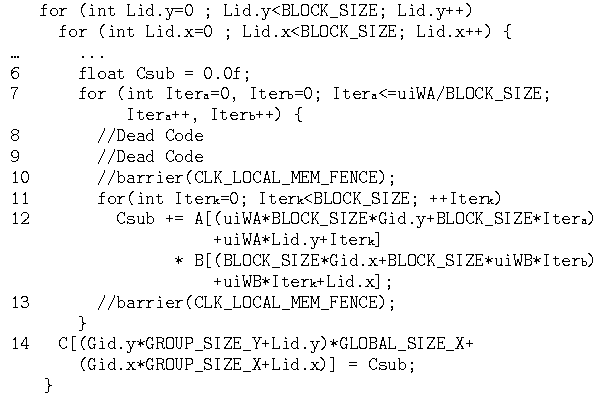
\includegraphics[width=10cm]{fig6.pdf}}	
	\label{debarriered}
\end{table}

消除同步语句之后,虽然其直接开销也被消除了,但是整个工作组的代码执行顺序也发生了改变。
图\ref{access}(a)显示了原GPU特定Kernel在执行过程中,一个工作组对于全局数组$\bm{A}$和$\bm{B}$的访问顺序。
其中粗箭头代表对数组元素的依次访问,黑色虚线箭头代表控制流。
由于采用分块矩阵乘法,$\bm{A}$的每一行分段会被连续访问16次,
$\bm{B}$的每一分块的各个行将以合并访存的方式被循环访问16次。
图\ref{access}(b)显示了工作项折叠后,线程循环的访问顺序。
矩阵乘法不再是分块的,对数组$\bm{A}$的访问将遍历整个行,对数组$\bm{B}$的访问将遍历整个列。
因此,Cache失效将不可避免,而且SIMD并行性无法得到开发。
这样的工作项折叠后代码虽然不够高效,但是十分``整齐'',有利于后继优化。
本章后继优化的目标不是还原图\ref{access}(a)所示的GPU特定的局部性,
而是根据目标CPU的体系结构细节,重新开发数据局部性和并行性。

%In Fig.~\ref{access}(c), each scalar element of $\bm{A}$ is expanded into a vector, and each set of eight adjacent accesses to $\bm{B}$ is vectorized to produce a new vector. Then computational operations are fully vectorized. In addition, the iterative array accesses are restricted in small blocks, so that the CPU cache can play a very good role.

\begin{figure}[htb]
\centering
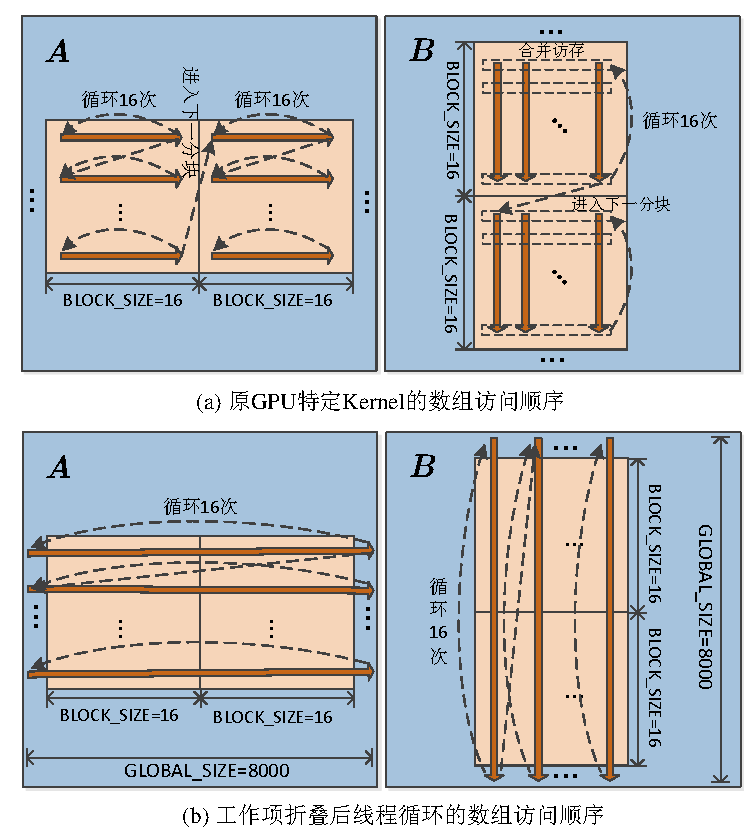
\includegraphics[width=12cm]{fig7.pdf}
\caption{矩阵乘法$\bm{C}=\bm{A}\times \bm{B}$中对于数组$\bm{A}$和$\bm{B}$的不同访问顺序}
\label{access}
\end{figure}


\section{适应体系结构的后继优化}
\label{postoptimizationsec}
完成工作项的折叠后,线程粒度大大变粗,工作组能够以线程循环的形式作为一个CPU线程进行执行。
但是此时仍然有两个CPU特定的性能要素没有得到利用。
一个是工作项间的并行性没有得到开发,导致CPU中的SIMD单元利用率低下。
另一个是线程循环的循环体过长,导致数据局部性不佳。
为此,本节将对折叠后的线程循环进行两步优化:向量化和局部性重开发。
这两步优化的目的在于,借鉴原GPU特定Kernel对于性能的考虑,针对CPU特定的体系结构细节提升代码性能。

\subsection{向量化}
对于工作项折叠后的线程循环,{\em icc}等高性能编译器能够进行自动向量化,以利用当前多核/众核CPU中广泛存在的SIMD单元。
但是,编译器通常只针对循环嵌套的最内层循环进行向量化\upcite{intelvectorguide},
而最内层循环可能无法向量化,或者不是进行向量化的最佳位置。
因此本节将不依赖编译器的自动向量化功能,而是显式地进行循环级的向量化优化。
这一过程不仅需要提取原GPU特定Kernel中的并行信息,同时还会考虑CPU的体系结构细节。

对于GPU来说,访问全局存储数组的最佳模式是顺序、逐个、对齐的访问\upcite{oclbestpractice}。
例如,第$k$个工作项访问对齐的全局存储段的第$k$个字。
这样的访存模式必然是合并访存,可以最大化地利用GPU的显存带宽。
GPU特定Kernel程序对于局部存储数组的访问通常也是顺序、逐个的(无需对齐),
目的是避免访存时发生组冲突。
此外,GPU还有一种高效的局部存储访问模式,即令同一Warp$/$半Warp内的工作项访问同一局部存储位置。

由于CPU体系结构下,OpenCL的全局存储和局部存储均对应于主存,
因此最适于进行向量化的循环层次就是以$Lid.x$为循环变量的循环。
原因在于,该层循环的相邻迭代对应于相邻的工作项。
而相邻工作项顺序、逐个的访存模式正好可以转换为向量加载指令(Vector-Load)和向量存储指令(Vector-Store);
相邻工作项访问同一存储位置的访存模式也可以转化为置向量指令(Vector-Set)或向量广播指令(Broadcast)。
除了访存操作以外,各种数学操作都可以通过经典的循环向量化方法无障碍地进行向量化,因为$Lid.x$循环在工作项折叠之后,
没有任何循环间依赖。

对于工作项折叠后的代码的向量化步骤如下:
\begin{compactitem}
\item[1)]{如果原GPU特定Kernel程序中包含循环,则进行循环分布(Loop Distribution),使得非线程循环(即循环变量不是工作项索引的循环)成为循环嵌套的最内层循环。该步骤可能需要变量扩展,并会导致更多的循环控制语句。但是相比向量化后的巨大性能提升,这些额外开销是可忽略的。}
\item[2)]{对于每一个循环嵌套,进行循环交换(Loop Interchange),使得$Lid.x$循环成为循环嵌套的最内层循环。这一步骤一定是可进行的,因为线程循环的循环层间没有任何依赖。}
\item[3)]{根据目标CPU体系结构的SIMD单元宽度,对$Lid.x$循环进行循环分段(Loop Blocking),使得得到的循环嵌套的外层循环变量(记为$vLid.x$ )以(SIMD单元宽度$/$数组元素宽度)为步长。之后即可按经典方法对最内层循环进行向量化。假设用于计算的是单精度浮点数(32位),对于Sandy Bridge架构的CPU,由于SIMD宽度为256位,循环步长设为8。而对于Knights Corner架构的MIC协处理器,由于SIMD宽度为512位,循环步长设为16。此外Knights Corner架构还包括了向量乘加单元(FMA),因此其编译器可以自动地将乘法和加法融合。}
\end{compactitem}

工作项折叠后的矩阵乘法Kernel代码,再经过向量化,变为如表\ref{vectorized}所示。
表中假设CPU的SIMD宽度为256位,所示的$vLid.x$是经过了循环正规化的。
前缀``vec''代表向量数据类型或者向量操作。
可以看出,$Lid.x$循环被分段后得到的3个循环嵌套中,最内层的循环都已经因为完全向量化而消失了。

\begin{table}[htb]
\centering
\caption{向量化后的矩阵乘法Kernel代码片段}
\fbox{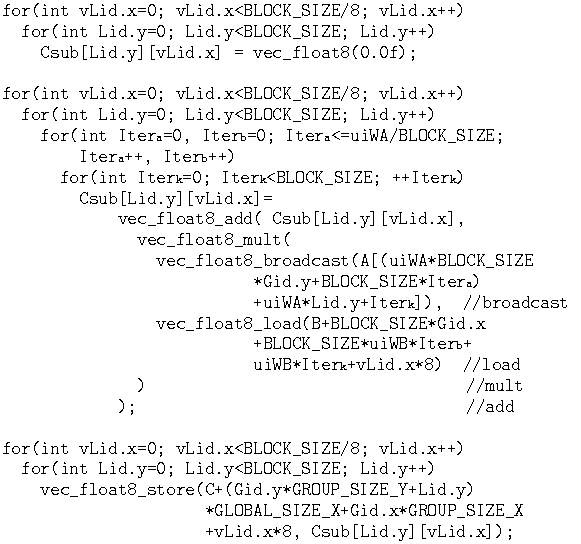
\includegraphics[width=10cm]{fig8.pdf}}
\label{vectorized}
\end{table}

\subsection{局部性重开发}
\label{localityreexploresec}
经过工作项折叠和向量化,转换得到的Kernel程序的并行性已经非常适合CPU体系结构。
但是,数据局部性仍然没有得到改善。
大部分的GPU特定Kernel程序在实现时都考虑了数据局部性,例如将长循环分段等。
但是有的Kernel程序并没有进行相关优化。例如\cite{oclprogrammingguide}中给出的``基本矩阵乘法Kernel'',
它和上文中讨论的矩阵乘法Kernel具有相同的功能,但是没有进行任何局部性优化,因此被Nvidia作为一个基准程序来展示局部存储的作用。
本节的局部性重开发方法会利用到原GPU特定Kernel对于局部性的优化,但同时也会尽量适应目标CPU体系结构对数据局部性的需求,
因此即使是数据局部性很差的GPU特定Kernel,仍然可以通过本节的方法在CPU上获得极大性能提升。
本节使用(并微调)了经典的循环级优化方法,包括循环交换、循环分段和提升寄存器重用率。
具体的数据局部性重开发方法分为以下3个步骤。

{\bf 1)\ 将非线程循环分段。} 主要思想是:如果一个循环的循环变量出现在了一个多维数组的最低维(该维度的相邻元素在内存中连续)索引中,且不出现在其它维度的索引中,那么对该循环进行分段通常是有好处的\upcite{compilerbook}。
对于所有的非线程循环,如果同时满足下面两个条件,则对其进行分段:
\begin{compactitem}
\item[a)]{循环体中某个数组访问对应的线性描述式包含了非线程循环的循环变量,且该循环变量的系数足够小;(这里以2作为保守的阈值,因为太大的系数会导致访存模式的步长较大,从而限制循环分段的有效性。)}
\item[b)]{对于a)中的数组访问,将一次循环迭代的元素访问范围转换为字节数,得到访存覆盖范围足够大。(这里使用一个经验阈值,即L1 Cache大小的$1/8$,因为如果每次迭代的访存范围很窄,则无需进行循环分段。对于Sandy Bridge和Knights Corner架构,该阈值均为4KB。)}
\end{compactitem}
如果需要进行循环分段,非线程循环将被转换为两个嵌套的循环,并且内层循环的迭代次数(Trip Count)将被设置为工作组最低维的工作项数目,即$Lid.x$的取值范围大小。
经典的循环分段包括两个步骤,分段开采和循环交换。但是这里的循环分段只进行分段开采,而不考虑循环交换。
循环交换将在下一步骤中,针对所有层次的循环(包括线程循环)同时进行。
如表\ref{vectorized}的中间部分所示,${Iter_k}$循环和${Iter_a/Iter_b}$循环实际上已经是非线程循环被分段后得到的内、外层循环了,
因此没有非线程循环满足上述分段条件。
但是,``基本矩阵乘法Kernel''中的$k$循环会被检测出来并进行分段处理。

{\bf 2)\ 循环交换。} 这里将沿用Allen等人提出的启发式循环交换算法\upcite{compilerbook}。
对于嵌套的多个循环$\{ {L_1}, {L_2},\ldots ,{L_n} \}$,首先建立一个启发式函数,用于估计循环嵌套中的数组访问(包括向量加载和存储)可能导致的Cache失效次数。
然后对于每一层循环${L_i}$,假设其处于最内层,用启发式函数估计出循环嵌套的Cache失效次数(称作该循环的最内层存储开销),记为$C_M({L_i})$。
最后,各层循环按照$C_M$值的降序,从内到外进行重新排列。

但是,上述循环交换算法在计算$C_M$值时基于一个重要假设,即当前循环的迭代次数是无限大的。
而线程循环和分段后的内层非线程循环的迭代次数通常较少,因此上述算法还需要修改:
当计算一个循环的最内层存储开销(即$C_M$值)时,如果它的迭代次数少于工作组最低维的工作项数目,则不再把它的失效次数乘以它外层循环的迭代次数。
上述算法有的时候还会产生多个循环交换方案,例如表\ref{vectorized}中间部分的嵌套循环中,
${Iter_a/Iter_b}$循环应当被置于最外层,${Iter_k}$循环应当被置于最内层,而${vLid.x}$循环和${Lid.y}$循环的位置是可以互相交换的。

{\bf 3)\ 选择利于向量寄存器重用的循环交换。} 单个CPU核里的向量寄存器是非常稀有的计算资源。Sandy Bridge架构中有16个,
Knights Corner架构中有32个。因此向量寄存器的重用率将对Kernel性能产生很大影响。
提升寄存器的重用率实际上就是提升Kernel的数据时间局部性,故这里仍然利用上一步中计算$C_M$值的启发式函数,
并针对时间局部性进行修改:
每一个向量操作都被看作是``访存操作'',Cache大小设置为向量寄存器的数量,Cache行的长度设置为$1$。
这样一来,修改后的启发式函数估计出的``Cache失效次数''实际上是向量寄存器的溢出次数。
将该启发式函数应用于上一步得到的所有循环交换方案,$C_M$值最小的方案就是向量寄存器重用率最高的循环交换。
再次观察表\ref{vectorized}中间部分的嵌套循环,如果一个CPU核包含16个256位的向量寄存器,
那么将${vLid.x}$循环置于${Lid.y}$循环之外将获得更佳的时间局部性。

经过局部性重开发后的矩阵乘法Kernel代码片段如表\ref{cpuoutput}所示(仅显示了Kernel中间的循环嵌套),
它同时也是将GPU特定Kernel面向Sandy Bridge架构的CPU转换所得到的最终结果。
对于数组$\bm{A}$和$\bm{B}$的访问顺序也变为图\ref{access2}所示。
可以看出,原GPU特定Kernel中的合并访存转换为了向量操作,数据局部性也得到了大幅提升。

\begin{table}[htb]
	\centering
	\caption{面向Sandy Bridge架构转换后的最终矩阵乘法Kernel代码片段}
	\fbox{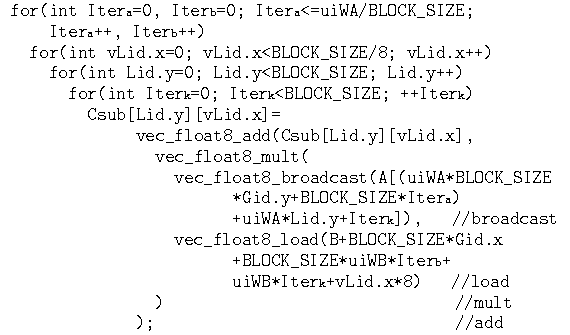
\includegraphics[width=10.5cm]{fig9.pdf}}
	\label{cpuoutput}
\end{table}

\begin{figure}[htb]
\centering
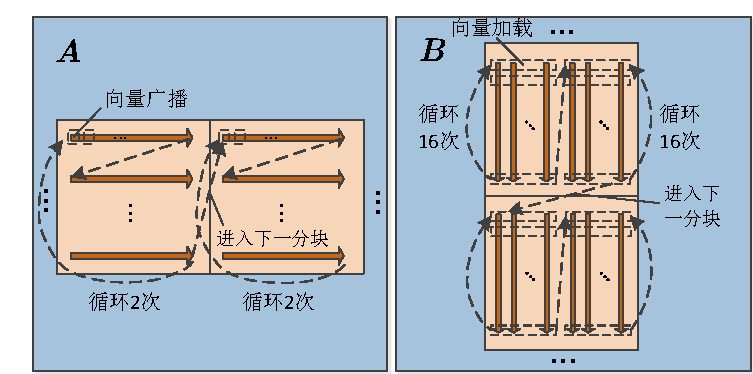
\includegraphics[width=12cm]{fig72.pdf}
\caption{转换后的矩阵乘法Kernel对于数组$\bm{A}$和$\bm{B}$的访问顺序}
\label{access2}
\end{figure}

表\ref{micouput}显示了将GPU特定Kernel面向Knights Corner架构的MIC转换所得到的最终结果。
其中${vLid.x}$循环和${Lid.y}$循环的位置可以互换,不影响性能。
表\ref{micouput}和表\ref{cpuoutput}有区别的原因在于不同的SIMD宽度、是否有FMA单元、以及不同的向量寄存器数量。


\begin{table}[htb]
\centering
\caption{面向Knights Corner架构转换后的最终矩阵乘法Kernel代码片段}
\fbox{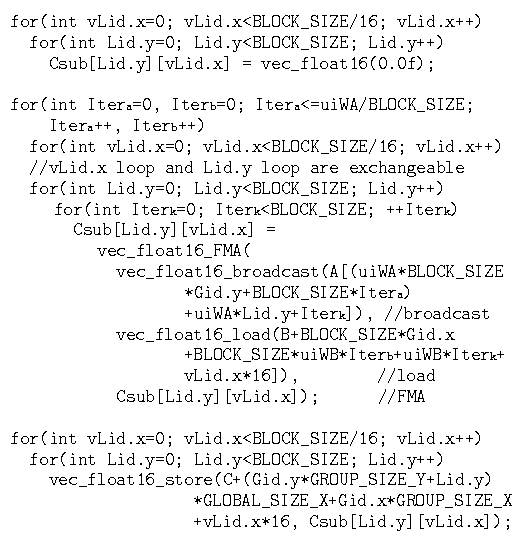
\includegraphics[width=10cm]{fig10.pdf}}
\label{micouput}
\end{table}


\section{运行时调度}
\label{runtimesec}
上述的整个代码转换过程,包括提取数组访问描述式,消除冗余的局部存储数组和同步语句,构建线程循环,
以及后继优化,被实现为一个源到源的代码转换工具链。
该工具链基于Clang\upcite{clang}编译器前端,以及LLVM\upcite{llvm}中间代码转换库。
通过工具链的转换,再利用LLVM的CBE后端,GPU特定的OpenCL Kernel程序被转换为一个可链接的函数,
其输入参数为原Kernel的全部参数和工作组的组索引值。
每一次调用该函数,等价于执行了一个对应的工作组,也就是说,
进行运行时调度的粒度为单个工作组。

转换得到的Kernel代码不能直接被标准的OpenCL运行时调度运行。
因此需要一个配套的运行时调度器来调用转换后的函数。
该调度器的功能应类似于标准OpenCL运行时对工作组的调度。
本节实现调度器的主要思想是,将工作组尽可能连续地和均匀地分布到各个CPU核上执行,
即是说各个CPU核分到的工作组数量差别不超过$1$。
通过调度器,工作组间的并行性被转换为了线程级的并行性。

调度器执行Kernel的过程如下:
\begin{compactitem}
\item[1)]{主线程将所有工作组分成多个等量的集合,各个集合被连续地指派到目标多核/众核CPU的各个逻辑核上。
(由于超线程(Hyper Thread)技术,Sandy Bridge架构下一个物理核等价于两个逻辑核,而Knights Corner架构下一个物理核等于4个逻辑核,但这里忽略其第一个物理核,以用于执行主线程。)}
\item[2)]{主线程为每一个逻辑核创建一个POSIX线程,称作工作线程。
并通过设置线程的亲和属性(Affinity)来指定工作线程在对应逻辑核上运行。}
\item[3)]{各个工作线程根据被指派的工作组,不断地以工作组组索引值为参数调用转换后的函数。}
\item[4)]{主线程等待工作线程的汇聚(Join)。}
\end{compactitem}

利用工具链转换GPU特定Kernel的过程,以及转换后的代码通过调度器运行的过程都展示在了图\ref{sysdiagram}中。

\begin{figure}[htb]
	\centering
	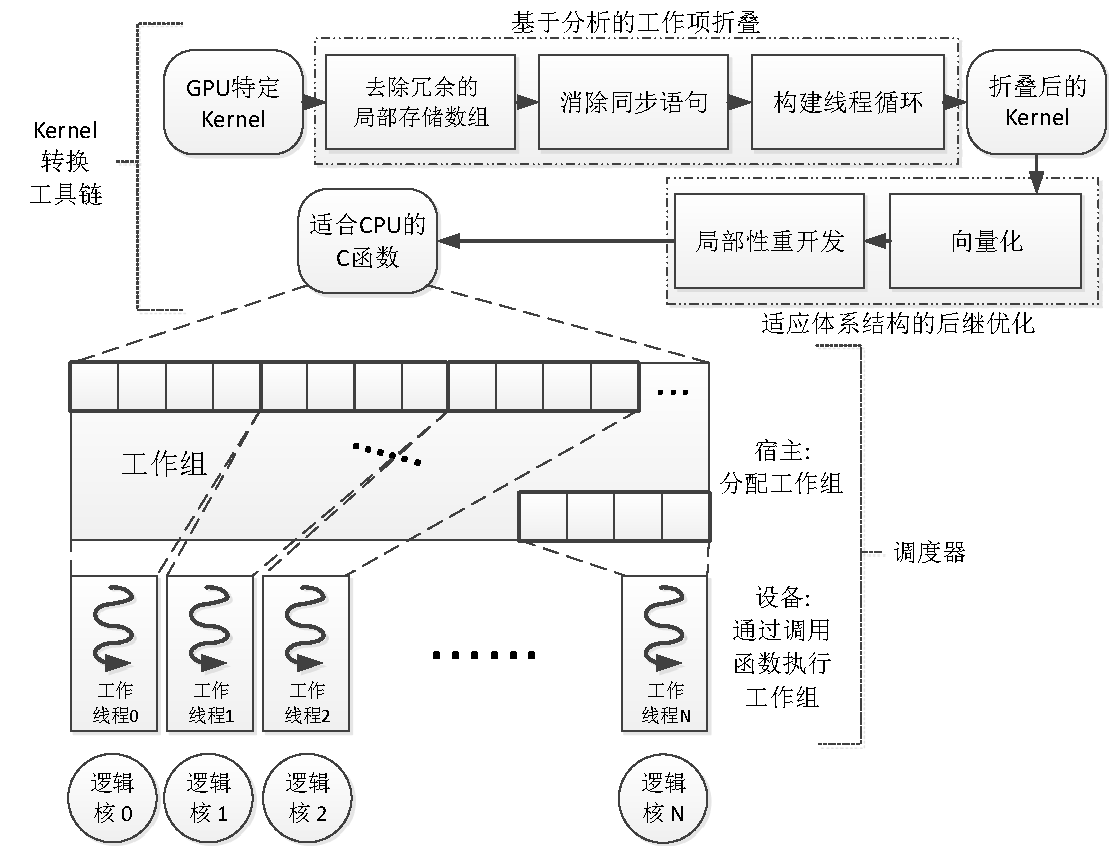
\includegraphics[width=13cm]{fig11.pdf}
	\caption{GPU特定Kernel的转换和调度执行}
	\label{sysdiagram}
\end{figure}

为了能够运行包括宿主程序和Kernel程序的完整OpenCL程序,本章的代码转换工具链和运行时调度器被集成到一个开源的OpenCL实现\pozhehao FreeOCL\upcite{freeocl}中。
原FreeOCL中的代码生成模块和Kernel调度模块被本章的代码转换工具链和调度器分别替换。
其它用于实现OpenCL宿主程序API的模块保持不变。
对于CPU和MIC,均使用Intel C++ Compiler v13.0.0编译转换后的Kernel代码。
在面向Sandy Bridge架构的CPU进行编译时,主要的编译选项为\texttt{-O3 -xHost}。
而对于Knights Corner架构的MIC,将在编译前需要为转换后的Kernel代码加上``offload''指导语句,使得整个Kernel程序可以在MIC上执行。
值得注意的是,由于本节在MIC上执行Kernel时使用的是卸载(Offload)模式,MIC的最后一个物理核将被保留,不可用于计算。
至此,包含GPU特定Kernel的OpenCL程序,将能够借助本章的新OpenCL运行时,在多核/众核CPU上高效地运行。

\section{性能评测}
\label{kernelexperimentsec}
本节将在两个硬件平台上进行实验和性能评测:
(1) 两个Intel Xeon E5-2650 8核CPU,共有16个物理核,作为经典的多核CPU平台;
(2) 一个Intel Xeon Phi 5110p MIC协处理器,共有60个物理核,作为新兴的众核CPU平台。
Xeon E5 CPU同时也作为宿主处理器,其上的操作系统为Red Hat Enterprise Linux 6.2,内核版本2.6.32-220。
本章提出的加入了Kernel转换工具链和运行时调度器的新OpenCL运行时(记作OurOCL),
将与Intel官方提供的OpenCL运行时(记作IntelOCL)进行对比。
Intel的官方OpenCL运行时来自Intel SDK for OpenCL Applications 2013\upcite{intelsdk}。

一共6个GPU特定的OpenCL Kernel程序组成了本节的测试集。
如表\ref{benchmarks}所示,前5个Kernel程序均针对GPU体系结构进行了高性能优化,
其中Stencil2D来自SHOC\upcite{shoc},其它4个来自Nvidia GPU Computing SDK。
第6个Kernel程序NaiveMatrixMul来自\cite{oclprogrammingguide},即\ref{localityreexploresec}节中介绍过的``基本矩阵乘法Kernel''。
它的数据局部性没有得到任何优化,将作为本节评测的基准。
值得注意的是,本节并没有选取上一章TLD算法高性能实现中的OpenCL Kernel作为测试集,原因主要有以下两点。
首先,本章的代码转换方法是一个通用方法,面向各类GPU特定的OpenCL Kernel程序。
而相比专用测试集中的Kernel,TLD算法中的Kernel程序所具有的代表性明显不足。
其次,上一章的Kernel程序中,有的包含间接访存(如Fern随机森林的特征提取和分类过程),因而无法使用本章方法;
有的未使用局部存储(如学习过程中的重叠率计算),
或者局部存储由于具有数据交换作用而无法去除(上一章所有使用了局部存储的Kernel程序),因而本章的方法无法完全发挥作用。
但是,本节选取的测试集和视觉跟踪仍然有着密切联系。
例如,KCF跟踪器中的所有逐元素操作都可以看做是Stencil2D的特例,
而离散余弦变换(DCT)也是KCF中离散傅里叶变换(DFT)的一种特殊形式。





\begin{table}[htb]
	\caption{用于性能评测的6个Kernel程序}
	\centering
	\scalebox{0.9} {
	\begin{tabular}{ p{2.7cm} p{3.7cm} p{2cm} p{6cm} }
		\toprule[1pt]
		Kernel名 & 数据规模 & 工作组大小      & 功能介绍\\
		\midrule[0.5pt]
		oclMatrixMul & $8000\times8000$ & $16\times16$ & 分块矩阵乘法\\
		%\hline
		\multirow{2}{*}{oclFDTD3d} & $320\times320\times320$,  & \multirow{2}{*}{$32\times32$} & \multirow{2}{*}{有限差分时域演化,三维模板计算}\\
		& Radius=16, Timestep=5	 &				&  \\
		%\hline
		\multirow{2}{*}{Stencil2D} & $4096\times4096$,  & \multirow{2}{*}{$16\times16$} & \multirow{2}{*}{标准的二维9点模板计算}\\
		& $1000$次迭代  &			  &		\\
		%\hline
		oclDCT8x8 & $10240\times10240$ & $32\times2$ &$8\times8$的离散余弦变换(DCT)\\
		%\hline
		oclNbody & $327680$ & $256$ & 327680个个体的引力模拟\\
		%\hline
		$*$NaiveMatrixMul & $8000\times8000$ & $16\times16$ & 未使用分块和局部存储的矩阵乘法\\
		\bottomrule[1pt]
	\end{tabular}
	}
	\label{benchmarks}
\end{table}

在Intel的产品平台上,IntelOCL通常是最为高效的OpenCL运行时。
一个Kernel依靠IntelOCL获得的性能通常也是最优的,即代表了``官方提供''的性能移植性。
因此通过对比同一Kernel在OurOCL和IntelOCL下的性能,即可评价两个运行时所提供的性能移植性。
上述的GPU特定Kernel程序在OurOCL下运行时,会先经过Kernel转换工具链的转换,然后被调度器调度运行。
同样的Kernel将在IntelOCL下再次运行,并对比两次运行所需的时间。
当运行Kernel程序时,本节仅记录Kernel执行的时间,而忽略其它开销。
通过Kernel的执行时间计算出的相对性能如表\ref{tointelocl}所示,
表中的所有相对性能都是相对于CPU+IntelOCL的性能比值。
此外,Kernel的绝对执行时间也显示在了括号里。
可以看出,在多核CPU平台上,GPU特定Kernel程序在OurOCL下的平均性能达到了IntelOCL下的3.24倍(不包括NaiveMatrixMul)。
而在众核MIC平台上,该平均性能比也达到了2.00倍。

\begin{table}[htb]
	\caption{与Intel OpenCL运行时和OpenMP的性能对比}
	\centering
	\scalebox{0.9}{
		\begin{tabular}{ p{0.9in} p{1in}<{\centering} p{1in}<{\centering} p{1in}<{\centering}  }
			\toprule[1.5pt]
			\multirow{2}{*}{Kernel}  & \multicolumn{3}{c}{相对性能 (执行时间)}\\ \cmidrule[1pt]{2-4}
			                      & CPU+IntelOCL& CPU+OurOCL& CPU+OMP\\
			\midrule[0.5pt]
			oclMatrixMul & 1 (23.30 s) & 3.02 (7.71 s) & 0.37 (62.98 s)\\
			%\hline
			oclFDTD3d & 1 (0.80 s) & 6.15 (0.13 s) & 2.16 (0.37 s)\\
			%\hline
			Stencil2D & 1 (20.65 s) & 2.53 (8.16 s) & 1.16 (17.80 s)\\
			%\hline
			oclDCT8x8 & 1 (75.96 ms) & 3.42 (22.20 ms) & 2.27 (33.46 ms)\\
			%\hline
			oclNbody & 1 (10.63 s) & 1.20 (8.82 s) & 0.74 (14.36 s)\\
			%\hline
			$*$NaiveMatrixMul & 1 (258.16 s) & 33.44 (7.72 s) & 4.10 (62.98 s)\\
			\bottomrule[1pt]
		\end{tabular}		
	}
		
	\hspace{0.005in} \scalebox{0.9}{
		\begin{tabular}{ p{0.9in} p{1in}<{\centering} p{1in}<{\centering} p{1in}<{\centering} }
			Kernel &  MIC+IntelOCL&	MIC+OurOCL&	MIC+OMP\\
			\midrule[0.5pt]
			oclMatrixMul &  1.94 (12.03 s) & 3.93 (5.93 s) & 3.74 (6.23 s)\\
			%\hline
			oclFDTD3d & 2.22 (0.36 s) & 5.71 (0.14 s) & 4.21 (0.19 s)\\
			%\hline
			Stencil2D & 1.83 (11.26 s) & 2.42 (8.53 s) & 1.95 (10.59 s)\\
			%\hline
			oclDCT8x8 &  1.43 (53.22 ms) & 4.18 (18.19 ms) & 4.52 (16.81 ms)\\
			%\hline
			oclNbody &  1.13 (9.44 s) & 1.24 (8.59 s) & 1.38 (7.70 s)\\
			%\hline
			$*$NaiveMatrixMul & 4.55 (56.73 s) & 43.76 (5.90 s) & 41.44 (6.23 s)\\
			\bottomrule[1.5pt]
		\end{tabular}			
	}
	\label{tointelocl}
\end{table} 

通过开发工作组间和工作项间的并行性,IntelOCL对于多处理器核和核内SIMD单元的利用非常高效。
但通过实验发现,它处理同步的开销处在分区域方法和Twin Peaks方法之间\upcite{TReporthIllinois}。
因此,OurOCL相比IntelOCL的性能提升应当主要来源于去除局部存储和同步,部分来源于对数据局部性的重开发。
Kernel程序oclNbody在两个硬件平台上的性能提升都是最小的,原因在于它的计算是最为密集的,
局部存储和同步导致的开销只占了执行时间的很小一部分。
两个模板计算Kernel(oclFDTD3d和Stencil2D)在MIC上的性能提升远低于在CPU上。
这是由于它们是高度访存密集的,只有少部分时间用于计算,而大部分时间用于访存,
因此MIC难以体现出并行计算能力的优势。
同样是由于访存过于密集,并且没有针对MIC的环状Cache互联进行优化,这两个Kernel在MIC上的性能(MIC+OurOCL)甚至低于它们在CPU上的性能(CPU+OurOCL)。
此外,因为多种开销的消除和数据局部性的大幅提升,NaiveMatrixMul在两个平台上均获得了可观的性能提升。

为了探究OurOCL可以将Kernel性能提升到何种程度,表\ref{tointelocl}也给出了各Kernel对应的OpenMP版本的相对性能。
这里的OpenMP版本来自于各Kernel的宿主程序中(用于检查Kernel执行结果的正确性),通过加入合适的OpenMP指导语句进行实现。
此外,在MIC上执行OpenMP程序时使用的是本地模式(Native Mode)。
上述的OpenMP版本并不是未优化的。一些Kernel的宿主程序,如oclDCT8x8,已经进行了CPU特定的局部性优化。
并且由于没有了OpenCL的语义限制,{\em icc}编译器也可以更加自由地进行多种自动优化。
从性能对比还可以看出,相比CPU,编译器为MIC进行的优化更为激进和有效。
因此,oclDCT8x8在MIC+OMP下的性能略高于它在MIC+OurOCL下的性能。
尽管oclNbody的OpenMP版本并没有像oclDCT8x8那样的专门优化,它在MIC下的性能仍然高于MIC+OurOCL。
目前其原因还尚不清晰,本节估计,这是因为oclNbody有着非常简单的且利于编译优化的访存模式,
同时MIC上OpenMP的调度方式要优于OurOCL的静态调度器。
总的来讲,无论在CPU还是MIC上,基于OurOCL的OpenCL Kernel性能接近于甚至优于OpenMP版本的性能。
这足以说明本章的代码转换方法和调度器可以减轻GPU特定Kernel中的负面性能要素,
并将性能提升到接近于适度优化的CPU特定程序。

图\ref{asf}显示了适应体系结构的后继优化中每一步带来的性能提升。
图中的纵坐标轴表示的是对应于各自原GPU特定Kernel的相对性能。
由于后继优化中的循环交换步骤只对CPU下的oclMatrixMul和NaiveMatrixMul产生了多个候选交换方案,
因此只有上图中的这两个Kernel才显示出最后一步优化。
其它的Kernel程序只有一种循环交换方案,因此略去了最后一步。
从图中可以看出,有的Kernel在折叠后由于数据局部性差以及并行性未被开发,性能急剧下降(oclMatrixMul、oclFDTD3d、oclNbody),
但是本章的后继优化将会激进地提取并行性并重开发局部性。
对于有的Kernel来说(Stencil2D、oclDCT8x8),去除局部存储和同步带来的性能提升抵消掉了折叠带来的局部性降低,因此在折叠后有着和原GPU特定Kernel接近或者更好的性能。
而本章的后继优化仍然能进一步提升这些Kernel的性能。

\begin{figure}[htb]
	\centering
 	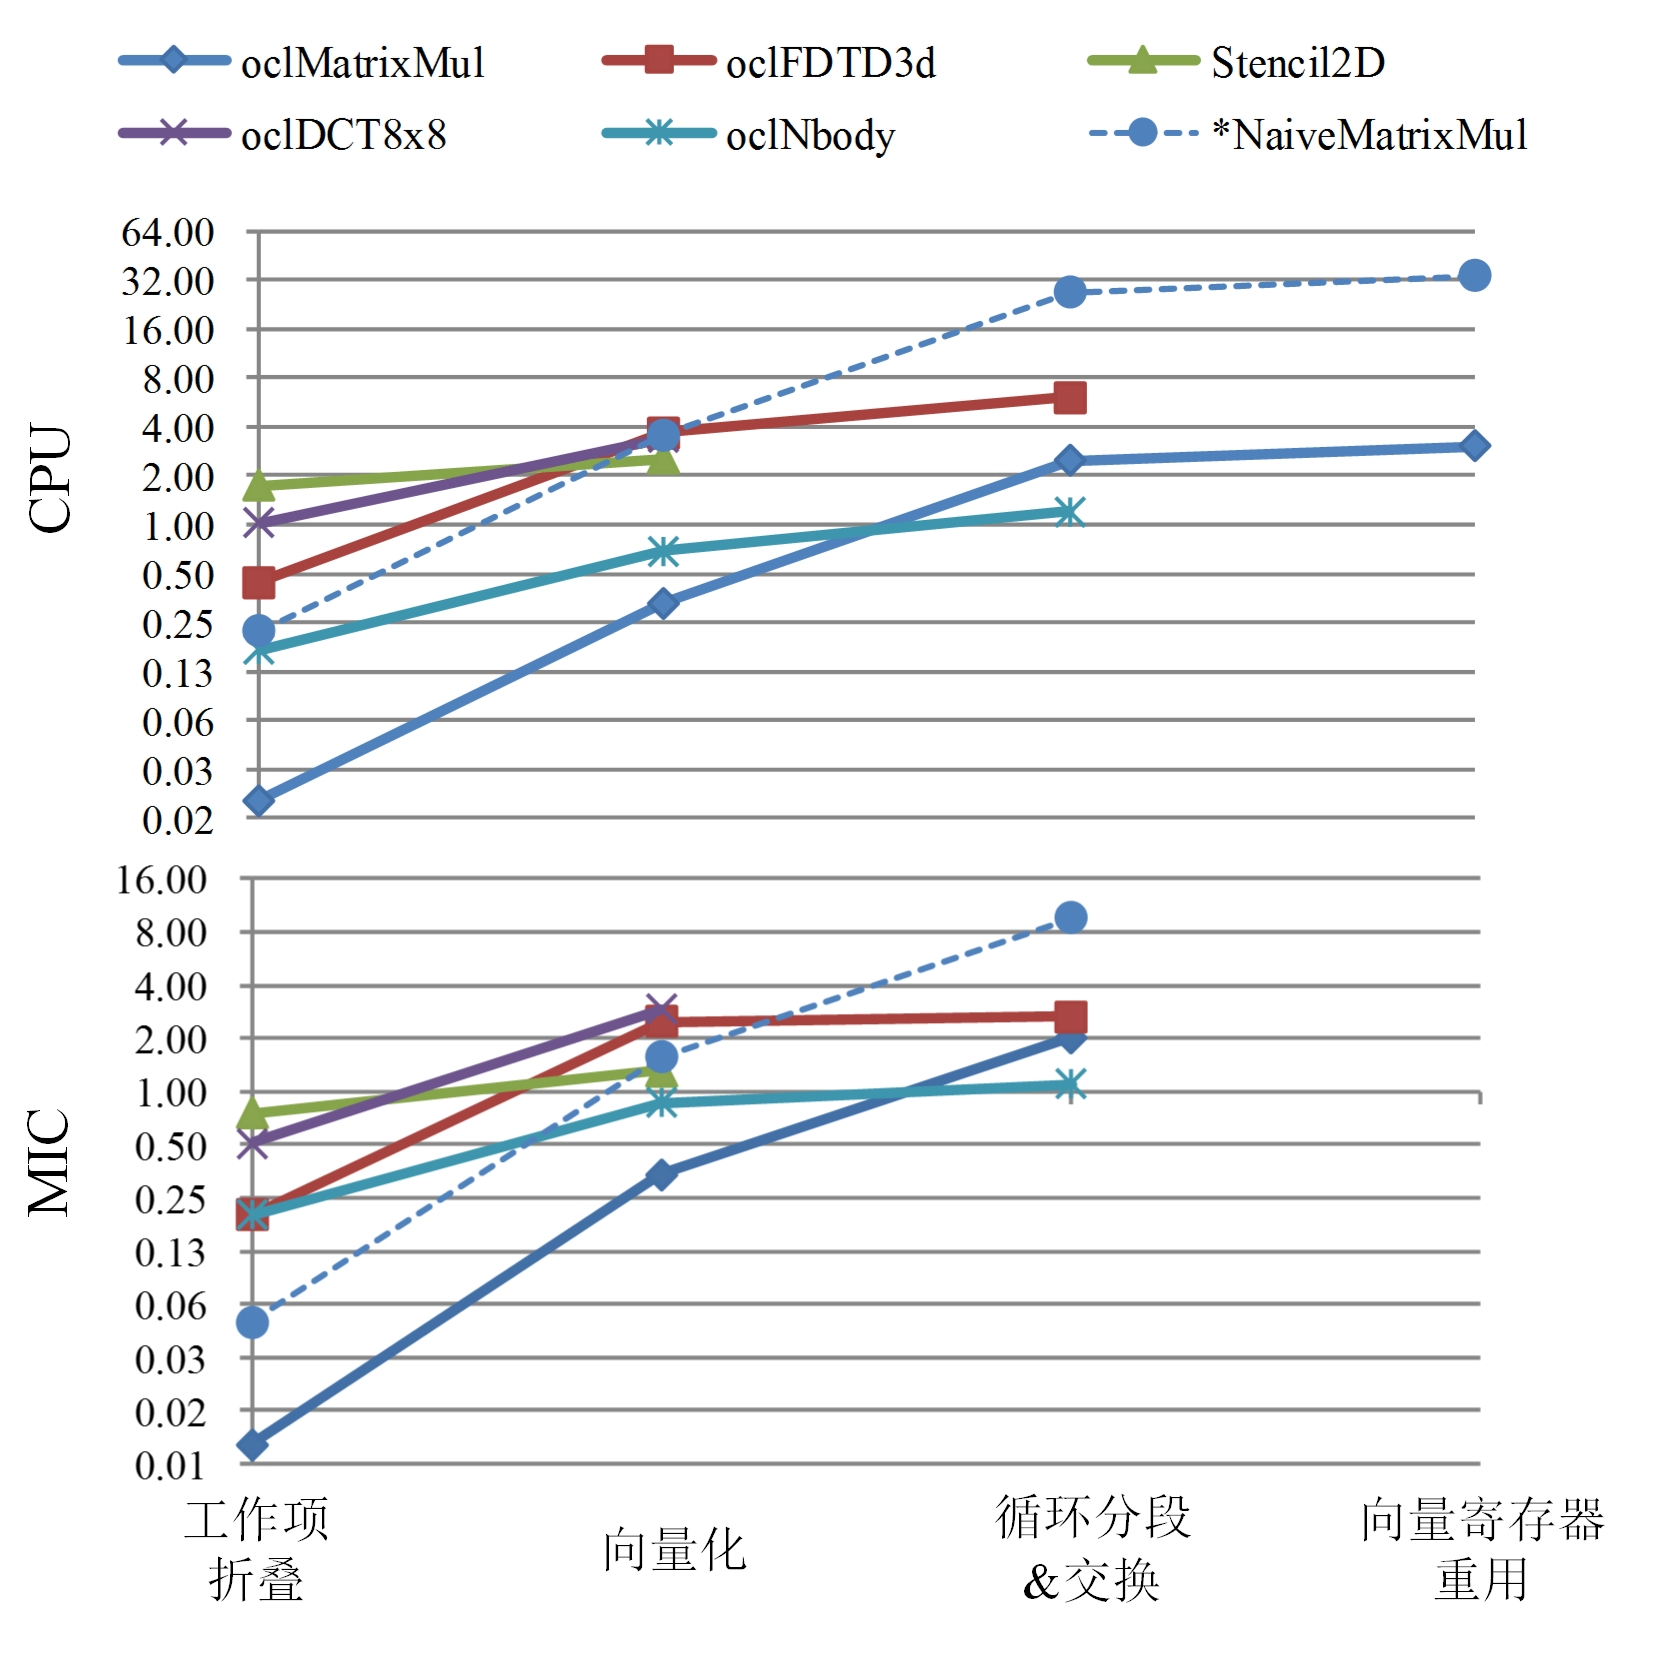
\includegraphics[width=11cm]{table3.jpg}
 	\caption{后继优化中各步骤带来的性能提升}
 	\label{asf}
 \end{figure}

根据图\ref{asf},向量化为oclMatrixMul和oclFDTD3d带来了巨大的性能提升,一些提升甚至超过了CPU的SIMD宽度。
原因在于向量化之前需要进行循环分布和交换,它们也会改变数据局部性,因此两种性能提升叠加在了一起。
但是,向量化对于oclNbody来说效果不明显,这是因为oclNbody中个体的速度和位置被紧邻地存储在一起,
即按``结构的数组''(Array of Structure)方式进行存储。
这将严重阻碍向量化的顺利进行。
NaiveMatrixMul的性能提升曲线和oclMatrixMul几乎一样,这是由于两者在工作项折叠后有着一样的控制流。
NaiveMatrixMul需要进行循环分段,而在循环分段后,两者的代码将变得相同。

\section{小结}
\label{kernelconclusionsec}
上一章中,通过在异构平台上基于OpenCL实现高性能TLD算法,OpenCL的性能移植性问题被暴露出来。
为此,本章进行了深入的探讨和解决。
本章提出了一套新的代码转换方法,该方法能够有效地提升GPU特定Kernel程序在多核/众核CPU上的性能移植性。
本章的方法解决了现有方法普遍忽略的两个重要问题:
一是在CPU上使用局部存储数组可能对性能带来负面影响,即额外的数据拷贝和同步开销;
二是忽视或者盲目继承GPU特定Kernel中的数据局部性特征,可能带来性能损失。
借助于本章新提出的数组访问描述式,在工作项折叠过程中,所有的冗余局部存储数组和对应的同步都将被消除。
后继优化过程中,本章不仅从原GPU特定Kernel中提取并行性和局部性特征,还会考虑目标CPU的体系结构细节,
以进一步提升Kernel程序在CPU上的性能。
实验显示,无论对于经典的多核CPU,还是新兴的众核协处理器MIC,包含本章方法的新OpenCL运行时都能取得超越Intel官方
运行时的性能。
借助本章的工作成果,在异构平台上实现高性能跟踪器时,可专注于面向GPU的优化,或是重用已有的GPU特定代码,
极大提高编程效率。
本章的方法仍然存在诸多不足,例如无法支持间接数组访问、静态调度算法不够高效、没有考虑工作组间的并行优化等。
未来将针对这些不足进行进一步的研究。
 

%*********************第六章******************
\chapter{总结与展望}
\section{工作总结}
本课题专注于异构计算的研究,无论是在高性能计算领域还是通用计算领域,异构计算都变得越来越重要了。本课题选取的两个应用分别是心脏模拟和深度学习领域比较热门的卷积神经网络应用。下面对这两个应用特点进行概述。

首先是心脏组织模拟应用的特点,归纳如下:

\begin{compactitem}
\item[1.]
主体计算是计算密集型。由于本课题采用的是非常精细的细胞模型,心脏细胞内结构复杂, 含有大量的dyad单元,每个dyad单元内又要模拟100多个通道,因此,心脏细胞内的计算量巨大,属于典型的计算密集型应用。虽然也有部分计算,比如细胞内dyad间电压的扩散过程,这是典型的stencil计算,这部分计算属于访存密集型的,但这部分计算只占细胞内所有计算时间的一小部分。因此,主要的计算类型是密集型计算。

\item[2.]
部分计算是控制语句主导的。对于细胞内的dyad单元的通道状态的模拟,按照直接的方法就是对每个dyad单元单独地进行模拟,每一个dyad单元中的通道状态模拟都涉及到中间计算结果与随机数的比较,比较控制语句在某些体系结构中是非常不高效的,比如在MIC加速器上,比较控制语句性能久很差。本课题采用的是二项分布随机采样模拟,这是一个随机采样的过程,对每个dyad的所有通道看作一个整体考虑,大大减少了控制比较语句的执行次数。不过还是无法完全避免所有的控制比较语句,所以这部分计算还是占了一定的开销。

\item[3.]
心脏组织的模拟具有多层并行性。心脏组织模拟应用表现出非常丰富的并行性,对计算的需求非常巨大,需要大规模并行系统才能满足。而心脏组织模拟的计算特点非常适合映射到大规模并行计算系统中,首先心脏组织被划分成规则的网格,每一个网格内的细胞计算由一个计算节点负责;其次,针对有多个加速器构成的异构节点,可以根据异构节点中主机CPU和加速器的计算性能比按比例将网格中的细胞进行划分;对于无论是多核CPU还是众核CPU负责的细胞计算,又可以采用OpenMP对细胞进行并行计算;最后每个小核在对单个细胞进行计算时,可以利用单核的SIMD特性对细胞内dyad单元进行向量化。

\item[4.]
心脏组织模拟如果需要模拟更加复杂的行为时,负载会出现不均衡的问题。如果需要模拟复杂的行为,需要给心脏组织的不同部位进行刺激,有时可能需要在不同的时刻进行刺激。由于刺激的细胞将电压传导到周围的细胞,那些已经被传导的细胞的行为与未被传导的细胞的行为是不同的,在模拟它们时所需计算量是有差异的。模拟的行为越复杂,心脏组织不同部位的模拟所需计算量的差异就越大,负载将变得越来越不均衡。本课题只模拟了简单的行为,因此,负载均衡问题不是特别突出。

\item[5.]
心脏组织模拟通信开销小。在心脏组织模拟应用中,发生在每个细胞内的计算相互独立,细胞间唯一发生联系的是细胞内的电压值,细胞内电压的计算与相邻细胞的电压值相关,因此,每个计算节点负责的网格细胞中处于外围的细胞的电压值都需要与处于相邻的网格外围细胞的电压值进行交换,每次时间迭代各个细胞的电压值都需要更新,因此,每个时间迭代步都涉及到电压值的通信。但相比每次迭代发生计算量,通信开销所占的比例是相当少的,这也是本课题在大规模节点中能取得很好扩展性的一个重要原因。

\item[6.]
精度敏感型。心脏组织模拟中采用精细的细胞模型,对精度要求极高,其中的变量都采用双精度浮点表示。高精度浮点计算将占用更多的计算资源,需要使用更宽的寄存器,意味着SIMD向量计算单元每次能处理的元素将变少。

\end{compactitem}

深度学习利用大量的训练数据对神经网络进行训练,在某些应用领域表现出了非常好的效果。现在比较流行的神经网络是卷积神经网络,目前各种卷积神经网络的设计表明,网络层次越深,精度越高,但问题就是带来计算量的增加。卷积神经网络涉及的计算与心脏组织模拟中的计算在某些方面具有相似的特点,比如都是计算密集型计算。但也表现出不一样的特点,具体如下:
\begin{compactitem}
\item[1.]核心计算其实就是矩阵乘运算。

\item[2.]前向计算过程对延迟要求低。

\item[3.]前向计算过程具有多种并行模式,不同并行模式涉及不同的通信模式。

\item[4.]大规模训练具有大规模计算节点的需求。

\item[5.]对数值表示的精度要求相对较低。
\end{compactitem}

卷积神经网络中的卷积计算虽然通过算法的改进可以降低浮点计算量,但核心计算部分仍然是矩阵乘运算,适合在异构平台上进行加速实现,本课题的改进算法中除了矩阵乘运算,还有部分计算主要涉及访存操作,是典型的访存密集型。

本课题针对这两种应用分别在两种不同的异构平台上进行映射实现。

\section{未来研究方向}




%

%%% Local Variables:
%%% mode: latex
%%% TeX-master: "../main"
%%% End:

\begin{ack}




\end{ack}


\cleardoublepage
\phantomsection
\addcontentsline{toc}{chapter}{参考文献}
\bibliographystyle{bstutf8}
\bibliography{ref/refs}

\begin{resume}

  \section*{发表的学术论文} % 发表的和录用的合在一起

  \begin{enumerate}[{[}1{]}]
  \addtolength{\itemsep}{-.36\baselineskip}%缩小条目之间的间距,下面类似
  \item Yang Y, Ren T L, Zhang L T, et al. Miniature microphone with silicon-
    based ferroelectric thin films. Integrated Ferroelectrics, 2003,
    52:229-235. (SCI 收录, 检索号:758FZ.)
  \item 杨轶, 张宁欣, 任天令, 等. 硅基铁电微声学器件中薄膜残余应力的研究. 中国机
    械工程, 2005, 16(14):1289-1291. (EI 收录, 检索号:0534931 2907.)
  \item 杨轶, 张宁欣, 任天令, 等. 集成铁电器件中的关键工艺研究. 仪器仪表学报,
    2003, 24(S4):192-193. (EI 源刊.)
  \item Yang Y, Ren T L, Zhu Y P, et al. PMUTs for handwriting recognition. In
    press. (已被 Integrated Ferroelectrics 录用. SCI 源刊.)
  \item Wu X M, Yang Y, Cai J, et al. Measurements of ferroelectric MEMS
    microphones. Integrated Ferroelectrics, 2005, 69:417-429. (SCI 收录, 检索号
    :896KM.)
  \item 贾泽, 杨轶, 陈兢, 等. 用于压电和电容微麦克风的体硅腐蚀相关研究. 压电与声
    光, 2006, 28(1):117-119. (EI 收录, 检索号:06129773469.)
  \item 伍晓明, 杨轶, 张宁欣, 等. 基于MEMS技术的集成铁电硅微麦克风. 中国集成电路, 
    2003, 53:59-61.
  \end{enumerate}

  \section*{研究成果} % 有就写,没有就删除
  \begin{enumerate}[{[}1{]}]
  \addtolength{\itemsep}{-.36\baselineskip}%
  \item 任天令, 杨轶, 朱一平, 等. 硅基铁电微声学传感器畴极化区域控制和电极连接的
    方法: 中国, CN1602118A. (中国专利公开号.)
  \item Ren T L, Yang Y, Zhu Y P, et al. Piezoelectric micro acoustic sensor
    based on ferroelectric materials: USA, No.11/215, 102. (美国发明专利申请号.)
  \end{enumerate}
\end{resume}

% 最后,需要的话还要生成附录,全文随之结束。
%\appendix
\backmatter
%% TeX
\chapter{模板提供的希腊字母命令列表}

大写希腊字母:
\begin{table}[htbp]
\centering
\begin{tabular}{llll}
\toprule
$\Gamma$~\verb|\Gamma| & $\Lambda$~\verb|\Lambda| & $\Sigma$~\verb|\Sigma| & $\Psi$~\verb|\Psi| \\
$\Delta$~\verb|\Delta| & $\Xi$~\verb|\Xi| & $\Upsilon$~\verb|\Upsilon| & $\Omega$~\verb|\Omega| \\
$\Theta$~\verb|\Theta| & $\Pi$~\verb|\Pi| & $\Phi$~\verb|\Phi| & \\
\midrule
$\varGamma$~\verb|\varGamma| & $\varLambda$~\verb|\varLambda| & $\varSigma$~\verb|\varSigma| & $\varPsi$~\verb|\varPsi| \\
$\varDelta$~\verb|\varDelta| & $\varXi$~\verb|\varXi| & $\varUpsilon$~\verb|\varUpsilon| & $\varOmega$~\verb|\varOmega| \\
$\varTheta$~\verb|\varTheta| & $\varPi$~\verb|\varPi| & $\varPhi$~\verb|\varPhi| & \\
\bottomrule
\end{tabular}
\end{table}

小写希腊字母:
\begin{table}[htbp]
\centering
\begin{tabular}{llll}
\toprule
$\alpha$~\verb|\alpha| & $\theta$~\verb|\theta| & $o$~\verb|o| & $\tau$~\verb|\tau| \\ 
$\beta$~\verb|\beta| & $\vartheta$~\verb|\vartheta| & $\pi$~\verb|\pi| & $\upsilon$~\verb|\upsilon| \\ 
$\gamma$~\verb|\gamma| & $\iota$~\verb|\iota| & $\varpi$~\verb|\varpi| & $\phi$~\verb|\phi| \\ 
$\delta$~\verb|\delta| & $\kappa$~\verb|\kappa| & $\rho$~\verb|\rho| & $\varphi$~\verb|\varphi| \\ 
$\epsilon$~\verb|\epsilon| & $\lambda$~\verb|\lambda| & $\varrho$~\verb|\varrho| & $\chi$~\verb|\chi| \\ 
$\varepsilon$~\verb|\varepsilon| & $\mu$~\verb|\mu| & $\sigma$~\verb|\sigma| & $\psi$~\verb|\psi| \\ 
$\zeta$~\verb|\zeta| & $\nu$~\verb|\nu| & $\varsigma$~\verb|\varsigma| & $\omega$~\verb|\omega| \\ 
$\eta$~\verb|\eta| & $\xi$~\verb|\xi| & $\varkappa$~\verb|\varkappa| & $\digamma$~\verb|\digamma| \\ 
\midrule
$\upalpha$~\verb|\upalpha| & $\uptheta$~\verb|\uptheta| & $\mathrm{o}$~\verb|\mathrm{o}| & $\uptau$~\verb|\uptau| \\ 
$\upbeta$~\verb|\upbeta| & $\upvartheta$~\verb|\upvartheta| & $\uppi$~\verb|\uppi| & $\upupsilon$~\verb|\upupsilon| \\ 
$\upgamma$~\verb|\upgamma| & $\upiota$~\verb|\upiota| & $\upvarpi$~\verb|\upvarpi| & $\upphi$~\verb|\upphi| \\ 
$\updelta$~\verb|\updelta| & $\upkappa$~\verb|\upkappa| & $\uprho$~\verb|\uprho| & $\upvarphi$~\verb|\upvarphi| \\ 
$\upepsilon$~\verb|\upepsilon| & $\uplambda$~\verb|\uplambda| & $\upvarrho$~\verb|\upvarrho| & $\upchi$~\verb|\upchi| \\ 
$\upvarepsilon$~\verb|\upvarepsilon| & $\upmu$~\verb|\upmu| & $\upsigma$~\verb|\upsigma| & $\uppsi$~\verb|\uppsi| \\ 
$\upzeta$~\verb|\upzeta| & $\upnu$~\verb|\upnu| & $\upvarsigma$~\verb|\upvarsigma| & $\upomega$~\verb|\upomega| \\ 
$\upeta$~\verb|\upeta| & $\upxi$~\verb|\upxi| & & \\ 
\bottomrule
\end{tabular}
\end{table}

希腊字母属于数学符号类别,请用\verb|\bm|命令加粗,其余向量、矩阵可用\verb|\mathbf|。


\end{document}
